%% Dokumentenvorspann für Aufgabenblatt Friesen Freitage
%%
%% (c) 2008 Carsten Lynker
%%
%% Abgeleitet aus einer früheren Klassenarbeitsvorlage
%%
%% Die einzelnen Aufgaben sind mit \aufgabe einzuleiten, die
%% Aufzählungsumgebung enumerate hat die in Klassenarbeiten
%% übliche Form a) ... b) ...
%%

\documentclass[11pt,parskip=half,a4paper]{scrartcl}
%\usepackage{ngerman}
%\usepackage[utf8]{inputenc}
\usepackage[T1]{fontenc}
\usepackage{multicol}
\usepackage{graphicx}
\usepackage{pslatex}
\usepackage{helvet}
\usepackage{listings}
\lstset{numbers=left, numberstyle=\tiny, numbersep=4pt, breaklines=true, frame=single, showstringspaces=false, basicstyle=\scriptsize}
% -*- latex -*-
% Definition of the Lua language for the listings package
% Time-stamp: <2008-11-30 15:27:16 rsmith>
% Written by Roland Smith <rsmith@xs4all.nl> and hereby placed in the public
% domain. 

\lstdefinelanguage{lua}
  {morekeywords={and,break,do,else,elseif,end,false,for,function,if,in,local,
     nil,not,or,repeat,return,then,true,until,while},
   morekeywords={[2]arg,assert,collectgarbage,dofile,error,_G,getfenv,
     getmetatable,ipairs,load,loadfile,loadstring,next,pairs,pcall,print,
     rawequal,rawget,rawset,select,setfenv,setmetatable,tonumber,tostring,
     type,unpack,_VERSION,xpcall},
   morekeywords={[2]coroutine.create,coroutine.resume,coroutine.running,
     coroutine.status,coroutine.wrap,coroutine.yield},
   morekeywords={[2]module,require,package.cpath,package.load,package.loaded,
     package.loaders,package.loadlib,package.path,package.preload,
     package.seeall},
   morekeywords={[2]string.byte,string.char,string.dump,string.find,
     string.format,string.gmatch,string.gsub,string.len,string.lower,
     string.match,string.rep,string.reverse,string.sub,string.upper},
   morekeywords={[2]table.concat,table.insert,table.maxn,table.remove,
   table.sort},
   morekeywords={[2]math.abs,math.acos,math.asin,math.atan,math.atan2,
     math.ceil,math.cos,math.cosh,math.deg,math.exp,math.floor,math.fmod,
     math.frexp,math.huge,math.ldexp,math.log,math.log10,math.max,math.min,
     math.modf,math.pi,math.pow,math.rad,math.random,math.randomseed,math.sin,
     math.sinh,math.sqrt,math.tan,math.tanh},
   morekeywords={[2]io.close,io.flush,io.input,io.lines,io.open,io.output,
     io.popen,io.read,io.tmpfile,io.type,io.write,file:close,file:flush,
     file:lines,file:read,file:seek,file:setvbuf,file:write},
   morekeywords={[2]os.clock,os.date,os.difftime,os.execute,os.exit,os.getenv,
     os.remove,os.rename,os.setlocale,os.time,os.tmpname},
   sensitive=true,
   morecomment=[l]{--},
   morecomment=[s]{--[[}{]]},
   morestring=[b]",
   morestring=[d]'
  }

\lstset{language=lua}
\usepackage[pdftitle={FlyWithLua Quick Reference Manual},pdfstartview={FitH},colorlinks=true]{hyperref}
\pdfcompresslevel=9
\pdfimageresolution=72

\usepackage{color}
\definecolor{hellgrau}{gray}{0.85}
\definecolor{dunkelgrau}{gray}{0.55}

\newcommand{\hinweis}[2]{%
\phantomsection\addcontentsline{toc}{section}{#1}
\begin{center}
\fcolorbox{dunkelgrau}{hellgrau}{\parbox{14cm}{\textbf{#1}#2}}
\end{center}
}

\newcounter{aufg}
\newcommand{\xsb}{XSquawkBox}
\newcommand{\punkte}[1]{\marginpar{\fcolorbox{dunkelgrau}{hellgrau}{\parbox{4.5ex}{\sffamily\tiny#1}}}}

\renewcommand{\labelenumi}{\alph{enumi})}

\newcommand{\aufgabe}{\stepcounter{aufg}\vspace{0.75cm}\pagebreak[3]{\phantomsection\addcontentsline{toc}{section}{Aufgabe~\arabic{aufg}}\Large\sffamily Aufgabe~\arabic{aufg}}}
\renewcommand{\labelenumi}{\alph{enumi})}

\usepackage{fancyhdr}
\usepackage{lastpage}
\pagestyle{fancy}
\lhead{}


\setlength{\headheight}{2cm}
\chead{
\includegraphics[width=2.0cm]{FlyWithLua_logo.jpg}\\[2ex]}
\cfoot{\footnotesize Page \thepage\ of \pageref{LastPage}}
\renewcommand{\headrulewidth}{0.4pt}
\renewcommand{\footrulewidth}{0.4pt}

%%%%%%%%%%%%%%%%%%%%%%%%
%% Ende des Vorspanns %%
%%%%%%%%%%%%%%%%%%%%%%%%

\hyphenation{values- HIDAPI-}

\begin{document}

\title{FlyWithLua V2.7.XX NG Reference Manual}
\author{Carsten Lynker}
\date{\today}

\maketitle
\vspace{2cm}

\begin{center}

\includegraphics[width=10cm]{FlyWithLua_logo.jpg}
\end{center}
\thispagestyle{empty}
\newpage
\verb||
\tableofcontents

\newpage
\section{Using the Plugin}
\subsection{What's needed}

To use FlyWithLua, you will need following:

\begin{enumerate}
\item The plugin itself.
\item A nice text editor (\href{http://www.vim.org/}{VIM}, \href{http://www.gnu.org/software/emacs/}{GNU Emacs}, \href{http://notepad-plus-plus.org/}{Notepad++}, ...).
\item The plugin >>\href{http://www.xsquawkbox.net/xsb/}{XSquawkBox}<< (optional, but usefull).
\item The plugin >>\href{http://wiki.x-plane.com/DataRefEditor}{DataRef Editor}<< (optional, but extremely high recommended).
\item Some skills in programming \href{http://www.lua.org}{Lua} (FlyWithLua uses \href{http://luajit.org/}{LuaJIT}, compatible to Lua 5.1).
\item Knowledge about \href{http://www.xsquawkbox.net/xpsdk/docs/DataRefs.html}{DataRefs}.
\end{enumerate}

\newpage
\subsection{Difference between Core, Complete, NG and Source Edition}

FlyWithLua is originally published in three different flavors but only the NG version is currently supported.

The first version is the \href{http://forums.x-plane.org/index.php?/files/file/35579-flywithlua-core-edition-for-x-plane-11-windows-linux-mac-os-x-version/}{Core Edition}. This is the right version to start your first steps in using Lua to customize your X-Plane installation. The Core Edition is fully supported by the FlyWithLua developer team and acts as the heart of the FlyWithLua economy. If you got an error with this version, check if you have the latest version installed and report your issue together with a \verb|Log.txt| and \verb|FlyWithLua_debug.txt| file at the official FlyWithLua support forum.

Please ask for support here: \href{http://forums.x-plane.org/index.php?/forums/forum/335-help-me-i-have-a-problem-with-flywithlua/}{HelpMe Forum of FlyWithLua}

The second edition was made for the user who know what they are doing. We call it the Complete Edition. \textbf{The Complete Edition is a ready to use binary version of FlyWithLua with additional libraries and no restrictions (access to private art control DataRefs is possible with this version).} Remember, Pandora keeps her box widely opened for you in the Complete Edition, but this has not only positive effects. The more possibilities you get to manipulate X-Plane, the more possible frustration may be the result, when Laminar Research updates X-Plane. If you do not know what the last sentence is about, you should not use the Complete Edition!

This version of FlyWithLua has a lower level of support. Please ask in the same \href{http://forums.x-plane.org/index.php?/forums/forum/335-help-me-i-have-a-problem-with-flywithlua/}{HelpMe Forum} to get some assistance.

The third edition was created to alow FlyWithLua to be used in VR and because of that effort can also be used on a second monitor. It has all the features of the previous Complete edition so can access private art control datarefs. The support is by the X-Plane org comunity and can be found here. Please ask in the same \href{http://forums.x-plane.org/index.php?/forums/forum/335-help-me-i-have-a-problem-with-flywithlua/}{HelpMe Forum} to get some assistance. 

For the real hackers we have the whole \href{https://github.com/X-Friese/FlyWithLua}{source code of FlyWithLua Core Edition} published on GitHub. Just grab the code and compile it for your own, to have the full control.

You want all menu entries blink in pink? If you are a C/C++ crack, just edit the source and compile your own flavor. FlyWithLua is published with the MIT license, so you can do everything you want to the source code without getting into trouble with us.

Years of hard work is our free gift to you. Use it with respect and honor.

\newpage
\subsection{Installation}

To use the plugin, just copy the complete folder \verb|FlyWithLua| into X-Plane's main plugin folder. The main plugin folder looks like this:

\emph{<<place where you store the sim>>}\verb|/X-Plane 10/Resources/plugins/|\footnote{If you use X-Plane 9 instead of X-Plane 10, search for the README\_XP9.txt file and follow the instruction inside.}

When the plugin starts up, there must be a folder named

\emph{<<place where you store the sim>>}\verb|/X-Plane 10/Resources/plugins/FlyWithLua/Scripts/|\footnote{If you rename the plugin, it will stop working. So never change it's folder name.}

with at least one file in it (no matter if it is a Lua script or not). When you copy the complete folder, you will start with two subfolders, \verb|Scripts| and \verb|Scripts (disabled)|. All scripts inside the \verb|Scripts| folder will be run automatically by the plugin.

When the plugin starts, it will run all files inside the \verb|Scripts| folder, who end as:

\verb|.fwl|, \verb|.FWL|, \verb|.lua|, \verb|.Lua| or \verb|.LUA|

If a file is hidden (it's name begins with a single dot), the file will be ignored by the plugin.

This means, you have three ways to disable a script.

\begin{enumerate}
\item Change the endian.
\item Hide it (let the name start with >>\verb|.|<<).
\item Move it to another folder.
\end{enumerate}

I prefer the last way, so you find the folder \verb|Scripts (disabled)| filled with examples. All these examples may produce an enormous frustration, if you just copy them into the >>active<< folder. They may redefine your joystick setting for example. So be very carefully and modify them before usage. Lua scripts are a powerful weapon!

\newpage
\subsection{How to interact with Lua}

If you have XSquawkBox\footnote{If not, you can click on the menu entry >>Enter a line of code<< in FlyWithLua's plugin menu. There is no need to have XSquawkBox installed to use FlyWithLua. On the other hand, flying online on VATSIM is really cool.} installed, there is an easy way to talk to Lua. If you type in a line into XSquawkBox starting with a \verb|>| (a greater than sign), the line is send directly to Lua, instead of talking to your VATSIM channel (on COM1). Try the following code:

\verb|>print(2+3)|

If everything is fine, Lua will print a \verb|5| into the XSquawkBox's main text display\footnote{Use the developer console to see the output, if you don't have XSquawkBox installed.}. The output produced by Lua is not forwarded to the VATSIM COM1 channel. So don't be afraid of disturbing the controller. You can check this behavior as XSquawkBox prints all internal information in dark red color.

So FlyWithLua is a little pocket calculator? Hmm, why not. But this is not the intension of the plugin. FlyWithLua was made to interact with DataRefs.

\subsection{Lua variables and DataRefs}

Lua can handle variables. You can try it out:

\verb|>LuaIsNice = true|\\
\verb|>print(LuaIsNice)|

Not very spectacular, but wait, let's tell Lua to bind a variable to a DataRef:

\verb|>DataRef("battery", "sim/cockpit/electrical/battery_on", "writable")|\\
\verb|>print(battery)|

Wow! Lua prints out a \verb|1| if the battery is on, or a \verb|0| when the battery is off. That's magic! But it goes even better. Turn on your plane and type this:

\verb|>battery = 0|

Plopp -- your plane is down. If a variable is connected to a DataRef, and you define the connection as not readonly (the third parameter of the function call was \verb|"writable"|),
all changes on the variable will be pushed to the DataRef instandly.

\subsection{Writing a first config file}

With the knowledge now, we can write a little config script like this:

\begin{lstlisting}
DataRef("pitch_nullzone", "sim/joystick/joystick_pitch_nullzone", "writable" )
pitch_nullzone = 0.0
DataRef("roll_nullzone", "sim/joystick/joystick_roll_nullzone", "writable" )
roll_nullzone = 0.0
DataRef("heading_nullzone", "sim/joystick/joystick_heading_nullzone", "writable" )
heading_nullzone = 0.0
\end{lstlisting}

This works very well, but it is not really user friendly. So I decided to give FlyWithLua some extra functions, who make the code more cheerful. The config file can be alternatively written as:

\begin{lstlisting}
set( "sim/joystick/joystick_pitch_nullzone",   0.0 )
set( "sim/joystick/joystick_roll_nullzone",    0.0 )
set( "sim/joystick/joystick_heading_nullzone", 0.0 )
\end{lstlisting}

Much easier to read, isn't it?

\subsection{Pre-defined variables}

But what to code if you want a nullzone of 0.1 in your piston, but 0.0 in your helicopter? You can use the pre-defined variable \verb|PLANE_ICAO|.

\begin{lstlisting}
-- nullzone of my little Cessna
if (PLANE_ICAO == "C172") then
   set( "sim/joystick/joystick_pitch_nullzone",   0.1 )
   set( "sim/joystick/joystick_roll_nullzone",    0.1 )
   set( "sim/joystick/joystick_heading_nullzone", 0.1 )
end
-- nullzone of my little coffee mill
if (PLANE_ICAO == "R22") then
   set( "sim/joystick/joystick_pitch_nullzone",   0.0 )
   set( "sim/joystick/joystick_roll_nullzone",    0.0 )
   set( "sim/joystick/joystick_heading_nullzone", 0.0 )
end
\end{lstlisting}

\subsection{Loop Callbacks}

All your code will be calculated automatically during startup, if you change the plane or position, or when you click on \verb|Reload all Lua script files| in the plugin's main menu.

If this is not enough to you, you can generate code, that will be calculated continuously in a loop callback.

These two commands given to Lua (using XSquawkBox's input line) will produce an ugly behavior:

\verb|>DataRef("poslight", "sim/cockpit/electrical/nav_lights_on", "writable")|\\
\verb|>do_sometimes("poslight = 0")|

Now, from time to time, Lua will turn off your navigation lights. Try it out to see how it works. You will not bewitch the simulator for the rest of your life. A simple click on the menu entry \verb|Reload all Lua script files| will reset your magic spell.

\subsection{Menu entries}

Every time you get your little bird back to \href{http://nav.vatsim-germany.org/files/edgg/charts/edlp/public/EDLP_ILS24.pdf}{Paderborn/Lippstadt (EDLP)}, you want to talk to the tower controller (on frequency 133.375) to initialize your VFR approach, and want your needle pointing to PAD (on frequency 354). Maybe you want to tune in the ILS signal.

You can define an ATC menu entry to script it. This will help a lot, because the code will only be calculated if you click on the menu entry. Nobody always want to fly around Paderborn, right? Write a little file like this and name it >>\verb|EDLP_VFR_Approach.lua|<<.

\begin{lstlisting}
DataRef("COM1", "sim/cockpit/radios/com1_freq_hz", "writable")
DataRef("NAV1", "sim/cockpit/radios/nav1_freq_hz", "writable")
DataRef("ADF1", "sim/cockpit/radios/adf1_freq_hz", "writable")

add_ATC_macro("coming home", [[-- fly home to EDLP
COM1 = 13337
NAV1 = 10855
ADF1 = 354]])
\end{lstlisting}

As the code of your macro needs more than one line, you use the double brackets \verb|[[| and \verb|]]| to write down a multi line string as the second argument of the function \verb|add_ATC_macro|. So don't forget the closing normal bracket, as shown in the last line above.

\subsection{Menu switches}

If you want to toggle a special behavior of your simulator, defined in a script, but you do not want to rename or move the file and reload all scripts to use it or not, you can use menu entry switches.

It's just as easy as giving Lua's \verb|add_macro| function two additional string parameters. Write a file like this and name it >>\verb|transponder_helper.lua|<<.

If you don't want to copy\&paste the code, just take a look into the \verb|Scripts (disabled)| folder.

\begin{lstlisting}
-- The groundspeed is in m/s (meter per second), not kn (knots), and always readonly
DataRef("groundspeed", "sim/flightmodel/position/groundspeed")
-- The transponder code is a 4-digit integer
DataRef("transponder_code", "sim/cockpit/radios/transponder_code", "writable")
-- Transponder mode (off=0,stdby=1,on=2,test=3)
DataRef("transponder_mode", "sim/cockpit/radios/transponder_mode", "writable")

-- we start in Europe most of the time
transponder_code = 7000

-- turn on your transponder when flying faster than 20 m/s (about 40 kn)
function check_transponder()
  if (transponder_help == true) then
    if ((groundspeed > 20) and (transponder_mode ~= 2)) then
      transponder_mode = 2
      XPLMSpeakString("Transponder set to active")
    end
    if ((groundspeed < 20) and (transponder_mode > 1)) then
      transponder_mode = 1
      XPLMSpeakString("Transponder set to standby")
    end
  end
end

-- check it every 10 sec
do_sometimes("check_transponder()")

-- make a switchable menu entry, default is on
add_macro("Automatically set Transponder", "transponder_help = true", "transponder_help = false", "activate")
\end{lstlisting}

\newpage
\section{Reference}
\subsection{Predefined variables}

All predefined variables are readonly. If you change them, X-Plane will not recognize it.

\subsubsection{LONGITUDE}

Gives the actual longitude value in decimal as a double float value (remember Lua didn't know float but only number). As X-Plane uses the data type \verb|double|, but the numbers in Lua are only \verb|float|, you will get an approximation.

The value is readonly, like all predefined variables. So it isn't possible to replace the plane in it's position by changing the value.

Positive values in LONGITUDE are east, negative values are west.

\subsubsection{LATITUDE}

This gives the latitude value of the plane's position as a decimal value. So for example seven degree thirty minutes north is represented as 7.5 (a positive value, negative values are south).

\subsubsection{PLANE\_ICAO}

A string holding the plane's ICAO code in it.

\subsubsection{PLANE\_TAILNUMBER}

The Tailnumber of the plane as a string.

\subsubsection{SCREEN\_WIDTH}

The screen width in pixel.

\subsubsection{SCREEN\_HIGHT}

The screen hight in pixel.

\subsubsection{MOUSE\_X}

Horizontally position of the mouse pointer. Coordinates start on the left side with 0 (zero).

\subsubsection{MOUSE\_Y}

Vertically position of the mouse pointer. Coordinates start on the bottom side with 0 (zero).

\subsubsection{XSB\_METAR}

A string containing the last metar received by XSquawkBox. If you are not connected to VATSIM, the variable will be useless. It is readonly.

Readonly means, you can't modify the online weather by changing the \verb|XSB_METAR| variable!

\subsubsection{LUA\_RUN}

An integer value showing how often Lua was (re)started. During the very first run of Lua, it's value is 1. You can use it to do things only once after X-Plane was started, and do not repeat when a new plane was loaded or the airport was changed. (Both will force a Lua restart.)

\subsubsection{XPLANE\_VERSION}

An integer value showing the version number of X-Plane. FlyWithLua is designed to run on X-Plane version 10.x, but it may run on X-Plane 9. To check if you are really on X-Plane 10 (or newer), you can say: \verb|if XPLANE_VERSION > 1000 then ... end|.

Example given: the version \href{http://wiki.x-plane.com/Beta#X-Plane_10.10_RC_3}{X-Plane 10.10rc3} shows: \verb|XPLANE_VERSION = 10101|

\subsubsection{XPLANE\_HOSTID}

An integer value showing the HostID of X-Plane, an OS-specific value (totally unnecessary).

\subsubsection{SDK\_VERSION}

An integer value showing the version number of the SDK, FlyWithLua is running on. The SDK version should be 210 or above for X-Plane 10. If not, download a version for X-Plane 10 of FlyWithLua.

\subsubsection{SYSTEM}

A string telling you on witch computer system FlyWithLua (the simulator) is running. It's value is \verb|"IBM"| on Windows systems, \verb|"APL"| on Apple Macintosh systems and \verb|"LIN"| on Linux systems.

\subsubsection{SYSTEM\_ARCHITECTURE}

A number either 32 or 64, depending on the architecture. 64 means X-Plane is running in 64-bit, 32 means the simulator and all plugins are running in 32-bit.

\subsubsection{XPLANE\_LANGUAGE}

A string value showing the language of X-Plane's menus. The value can be \verb|"English"|, \verb|"French"|, \verb|"German"|, \verb|"Italian"|, \verb|"Spanish"|, \verb|"Korean"|, \verb|"Russian"|, \verb|"Greek"|, \verb|"Japanese"|, \verb|"Chinese"| or \verb|"Unknown"|.

\newpage
Since FlyWithLua version 2.0 all menu entries are no longer forced to English. To create a multiple language support for your plugin, write code like this\footnote{All text other than English or German was translated using \href{http://translate.google.com/}{Google Translator}.}:

\begin{lstlisting}
dataref("COM1", "sim/cockpit/radios/com1_freq_hz", "writable")

if XPLANE_LANGUAGE == "German" then
   add_macro("Stelle das Funkgerät auf UNICOM", "COM1 = 12280")

elseif XPLANE_LANGUAGE == "French" then
   add_macro("Fréquence radio point sur l'UNICOM", "COM1 = 12280")

elseif XPLANE_LANGUAGE == "Spanish" then
   add_macro("Punto de frecuencia de radio en la UNICOM", "COM1 = 12280")

elseif XPLANE_LANGUAGE == "Italian" then
   add_macro("Punto di frequenza radio sulla UNICOM", "COM1 = 12280")

else
   add_macro("Set radio to UNICOM", "COM1 = 12280")
end
\end{lstlisting}

\subsubsection{DIRECTORY\_SEPARATOR}

A string containing the directory separator of the current OS.

\subsubsection{SYSTEM\_DIRECTORY}

The complete OS-specific path to the X-Plane root directory with trailing slash.

\subsubsection{SCRIPT\_DIRECTORY}

The complete OS-specific path to the scripts including a directory separator as it's last character. If you want to write a file named \verb|my_info.txt| into the scripts directory (instead of X-Plane's main directory), use code like this:

\verb|infofile = os.open(SCRIPT_DIRECTORY .. "my_info.txt", "w")|

\subsubsection{INTERNALS\_DIRECTORY}

The complete OS-specific path to the FlyWithLua Internals directory with trailing slash.

\subsubsection{MODULES\_DIRECTORY}

The complete OS-specific path to the FlyWithLua Modules directory with trailing slash.

\subsubsection{AIRCRAFT\_PATH}

The full path to your aircraft file, ending with a directory separator.

\subsubsection{AIRCRAFT\_FILENAME}

The name of the ACF aircraft file, including the endian "\verb|.acf|".

\subsubsection{DO\_EVERY\_FRAME\_TIME\_SEC}

The duration time in seconds of the every frame loop.

\subsubsection{DO\_EVERY\_DRAW\_TIME\_SEC}

The duration time in seconds of the drawing loop.

\subsubsection{DO\_SOMETIMES\_TIME\_SEC}

The duration time in seconds of the loop to be executed sometimes.

\subsubsection{DO\_OFTEN\_TIME\_SEC}

The duration time in seconds of the often executed loop.

\subsubsection{SCRIPTS\_LOADING\_TIME\_SEC}

The time it takes to load all scripts.

\subsubsection{CLOCKS\_PER\_SEC}

The number of clock ticks in one second, a C value depending on your system.

$\frac{1}{CLOCKS\_PER\_SEC}$ is the ninimal time that can be maesured.

\subsubsection{LUA\_MEMORY\_USAGE\_KB}

The memory usage of the Lua environment in kB. This is not the complete memory consumption of your scripts, as some objects like wave files are not stored into Lua, but are allocated in C by the plugin FlyWithLua.

\newpage
\subsection{Lua functions}

The following functions are written in core C++ and are a part of the plugin. Most of them are multi-defined to handle different count of arguments.

\subsubsection{DataRef( "\emph{variable name}", "\emph{DataRef name}" )}

\begin{enumerate}
	\item \emph{variable name} = Name of the Lua variable representing the DataRef.
	\item \emph{DataRef name} = Name of the DataRef. Look at the \href{http://www.xsquawkbox.net/xpsdk/docs/DataRefs.html}{listing of all DataRefs}.
\end{enumerate}

Binds a Lua variable to a DataRef\footnote{You can spell it \emph{dataref()} instead of \emph{DataRef()}, if you don't like uppercase letters.}. The connection will be forced to readonly. Not possible to array DataRefs.

\subsubsection{DataRef( "\emph{variable name}", "\emph{DataRef name}", "\emph{readonly}" )}

\begin{enumerate}
	\item \emph{variable name} = Name of the Lua variable representing the DataRef.
	\item \emph{DataRef name} = Name of the DataRef. Look at the \href{http://www.xsquawkbox.net/xpsdk/docs/DataRefs.html}{listing of all DataRefs}.
	\item \emph{readonly} = Should the variable be pushed to X-Plane when it is changed? Say \verb|"readonly"| to have it readonly or \verb|"writable"| to make it writable.
\end{enumerate}

Binds a Lua variable to a DataRef. The connection will be writealbe if you say \verb|"writable"| as the third argument and if the DataRef is writable. Not possible to array DataRefs.

\subsubsection{DataRef( "\emph{variable name}", "\emph{DataRef name}", "\emph{readonly}", \emph{index} )}

\begin{enumerate}
	\item \emph{variable name} = Name of the Lua variable representing the DataRef.
	\item \emph{DataRef name} = Name of the DataRef. Look at the \href{http://www.xsquawkbox.net/xpsdk/docs/DataRefs.html}{listing of all DataRefs}.
	\item \emph{readonly} = Should the variable be pushed to X-Plane when it is changed? Say \verb|"readonly"| to have it readonly or \verb|"writable"| to make it writable.
	\item \emph{index} = The index of an array DataRef.
\end{enumerate}

Binds a Lua variable to a DataRef. The connection will be writalbe if you say \verb|"writable"| as the third argument and if the DataRef is writable. For array DataRefs use a fourth argument, the index starting at 0 (Zero). It will bind the element at the given index. It will not bind an array as a Lua table.


\subsubsection{\emph{table} = dataref\_table( "\emph{DataRef name}")}

\begin{enumerate}
	\item \emph{table} = Name of the Lua variable representing the DataRef. The variable will be a Lua table, access it like an anrray with index starting at 0 (Zero). 
	\item \emph{DataRef name} = Name of the DataRef. Look at the \href{http://www.xsquawkbox.net/xpsdk/docs/DataRefs.html}{listing of all DataRefs}.
\end{enumerate}

This function will create a table variable to access a DataRef. You can use it for any type of DataRef, no matter if the DataRef is an array or not. Here are some examples:

\begin{lstlisting}
-- the battery DataRef is an array of up to 8 battery switches
battery = dataref_table("sim/cockpit2/electrical/battery_on")

-- now we turn on the first battery of the plane
battery[0] = 1

-- but it will work on non-array DataRefs too
COM1FREQ = dataref_table("sim/cockpit/radios/com1_freq_hz")

-- switch it to UNICOM
COM1FREQ[0] = 12280
\end{lstlisting}

\subsubsection{define\_shared\_DataRef("\emph{DataRef name}", "\emph{DataRef type}")}

\begin{enumerate}
	\item \emph{DataRef name} = Name of the DataRef. Look at the \href{http://www.xsquawkbox.net/xpsdk/docs/DataRefs.html}{listing of all DataRefs}.
	\item \emph{DataRef type} = Type of the DataRef. This type is a string argument and can be\\ \verb|"Int"|, \verb|"Float"|, \verb|"IntArray"|, \verb|"FloatArray"|, \verb|"Double"| or \verb|"Data"|.
\end{enumerate}

With this function you will create a DataRef of the given type if it does not exist. If it exist and the type is different, you will get an error message. If it still exists with the same type, this command will do nothing. Shared DataRefs should help you interacting with other plugins.


\subsubsection{\emph{table} = create\_dataref\_table( "\emph{DataRef name}", "\emph{DataRef type}")}

\begin{enumerate}
	\item \emph{table} = Name of the Lua variable representing the DataRef. The variable will be a Lua table, access it like an anrray with index starting at 0 (Zero). 
	\item \emph{DataRef name} = Name of the DataRef. Look at the \href{http://www.xsquawkbox.net/xpsdk/docs/DataRefs.html}{listing of all DataRefs}.
	\item \emph{DataRef type} = Type of the DataRef. This type is a string argument and can be\\ \verb|"Int"|, \verb|"Float"|, \verb|"IntArray"|, \verb|"FloatArray"|, \verb|"Double"| or \verb|"Data"|.
\end{enumerate}

Here you have the best way to create a new DataRef and connect it to a table variable inside Lua.

This is an example:

\begin{lstlisting}
-- A string must be created as a "Data" type
my_welcome_string = create_dataref_table("FlyWithLua/useless_samples/welcome", "Data")

-- no matter if it looks like a table, just index the first element to fill it
my_welcome_string[0] = "Hello World!"

-- another example, now we create an integer value
the_answer = create_dataref_table("FlyWithLua/useless_samples/the_answer", "Int")
the_answer[0] = 42

-- in times of alternative facts, we can have multiple answers
all_answers = create_dataref_table("FlyWithLua/useless_samples/answers", "IntArray")
all_answers[0] = 42
all_answers[1] = 2017
\end{lstlisting}


\subsubsection{\emph{DataRef name}, \emph{Index}, \emph{readonly}, \emph{DataRef type}, \emph{DataRef ID} = get\_DataRef\_binding( "\emph{variable name}" )}

\begin{enumerate}
	\item \emph{variable name} = Name of the Lua variable representing the DataRef.
	\item \emph{DataRef name} = Name of the DataRef. Look at the \href{http://www.xsquawkbox.net/xpsdk/docs/DataRefs.html}{listing of all DataRefs}.
	\item \emph{Index} = The Index of the DataRef. This is always 0 (zero) if the DataRef isn't an array.
	\item \emph{readonly} = This results to \verb|true| is the DataRef is readonly and \verb|false| if it's writable.
	\item \emph{DataRef type} = Type of the DataRef. 1 = integer, 2 = float, 4 = double, 8 = float array, 16~=~integer array and 32 = data (strings).
	\item \emph{DataRef ID} = The ID of the DataRef. A pointer to the memory, the DataRef is stored.
\end{enumerate}


\subsubsection{button( \emph{button number} )}

\begin{enumerate}
	\item \emph{button number} = Number of the button, starting at 0 (zero).
\end{enumerate}

Returns the value of the actual state of a joystick button. \verb|button(i)| will result in \verb|true| if the button is pressed, else it gives back \verb|false|. The argument \verb|i| must be an integer, ranging from 0 to 1599. Check out the number in X-Plane's advanced buttons menu.

\subsubsection{last\_button( \emph{button number} )}

\begin{enumerate}
	\item \emph{button number} = Number of the button, starting at 0 (zero).
\end{enumerate}

Returns the value of the state of a joystick button, as it was during the last frame. \verb|last_button(i)| will result in \verb|true| if the button was pressed, else it gives back \verb|false|. The argument \verb|i| must be an integer, ranging from 0 to 1599. Check out the number in X-Plane's advanced buttons menu.

\textbf{Advice:}\\
Always use \verb|button()| and \verb|last_button()| to grab joystick values, instead of using\\ \verb|DataRef("MyButton", "sim/joystick/joystick_button_values", "readonly", 123)|, if you like super fast code execution. The functions \verb|button()| and \verb|last_button()| deliver values much efficient than user defined DataRefs.

\subsubsection{create\_switch( \emph{button number}, \emph{DataRef name}, \emph{index}, \emph{off value}, \emph{on value} )}

\begin{enumerate}
	\item \emph{button number} = Number of the button, starting at 0 (zero).
	\item \emph{DataRef name} = Name of the DataRef. Look at the \href{http://www.xsquawkbox.net/xpsdk/docs/DataRefs.html}{listing of all DataRefs}.
	\item \emph{index} = The index of an array DataRef, else 0.
	\item \emph{off value} = Value to be set when button is not pressed (off).
	\item \emph{on value} = Value to be set when button is pressed (on).
\end{enumerate}

This will turn a joystick buton into a switch controlling a DataRef. If the button is not pressed, the DataRef will be set to the off value, else to the on value. The index is 0 (zero) for non-array DataRefs.

The last three arguments are optional. If you leave them away, Lua will guess 0 for the index and the off value and 1 for the on value. So this will be fine to let button no.~15 control the battery as a real hardware switch:

\verb|>create_switch(15, "sim/cockpit/electrical/battery_on")|

\subsubsection{create\_positive\_edge\_flip( \emph{button number}, \emph{DataRef name}, \emph{index}, \emph{first value}, \emph{second value} )}

\begin{enumerate}
	\item \emph{button number} = Number of the button, starting at 0 (zero).
	\item \emph{DataRef name} = Name of the DataRef. Look at the \href{http://www.xsquawkbox.net/xpsdk/docs/DataRefs.html}{listing of all DataRefs}.
	\item \emph{index} = The index of an array DataRef, else 0.
	\item \emph{first value} = Value to be set when button is just pressed (positive edge detecttion).
	\item \emph{second value} = Value to be set when button is just pressed but the DataRef's value is equal to the first value.
\end{enumerate}

This is similar to the \verb|create_switch()| function, but it will flip between the two values, given as the last two arguments, every time a positive edge was detected (when the button is pressed just in that moment).

The last three arguments are optional. If you leave them away, Lua will guess 0 for the index and the first value and 1 for the second value. So this will be fine to let button no.~15 control the battery and flip it every time it is pressed:

\verb|>create_positive_edge_flip(15, "sim/cockpit/electrical/battery_on")|

Lua will automatically handle it like this:

\verb|>create_positive_edge_flip(15, "sim/cockpit/electrical/battery_on", 0, 0, 1)|


\subsubsection{create\_negative\_edge\_flip( \emph{button number}, \emph{DataRef name}, \emph{index}, \emph{first value}, \emph{second value} )}

\begin{enumerate}
	\item \emph{button number} = Number of the button, starting at 0 (zero).
	\item \emph{DataRef name} = Name of the DataRef. Look at the \href{http://www.xsquawkbox.net/xpsdk/docs/DataRefs.html}{listing of all DataRefs}.
	\item \emph{index} = The index of an array DataRef, else 0.
	\item \emph{first value} = Value to be set when button is just released (positive edge detecttion).
	\item \emph{second value} = Value to be set when button is just released but the DataRef's value is equal to the first value.
\end{enumerate}

Nearly the same as the function \verb|create_positive_edge_flip()|, but it will react when the button is released. For an engeneer, this is the negative edge of the button's signal.

\subsubsection{create\_positive\_edge\_trigger( \emph{button number}, \emph{DataRef name}, \emph{index}, \emph{value} )}

\begin{enumerate}
	\item \emph{button number} = Number of the button, starting at 0 (zero).
	\item \emph{DataRef name} = Name of the DataRef. Look at the \href{http://www.xsquawkbox.net/xpsdk/docs/DataRefs.html}{listing of all DataRefs}.
	\item \emph{index} = The index of an array DataRef, else 0.
	\item \emph{value} = Value to be set in the moment when button is pressed down (positive signal edge).
\end{enumerate}

This will set the DataRef to the given value in the moment, when the button is pressed down, not during hold. In engineer's words it's a positive edge detection.

\subsubsection{create\_negative\_edge\_trigger( \emph{button number}, \emph{DataRef name}, \emph{index}, \emph{value} )}

\begin{enumerate}
	\item \emph{button number} = Number of the button, starting at 0 (zero).
	\item \emph{DataRef name} = Name of the DataRef. Look at the \href{http://www.xsquawkbox.net/xpsdk/docs/DataRefs.html}{listing of all DataRefs}.
	\item \emph{index} = The index of an array DataRef, else 0.
	\item \emph{value} = Value to be set in the moment when button is released (negative signal edge).
\end{enumerate}

This will set the DataRef to the given value in the moment, when the button is released. In engineer's words it's a negative edge detection.


\subsubsection{create\_positive\_edge\_increment( \emph{button number}, \emph{DataRef name}, \emph{index}, \emph{stepping}, \emph{limit}, \emph{rounding} )}

\begin{enumerate}
	\item \emph{button number} = Number of the button, starting at 0 (zero).
	\item \emph{DataRef name} = Name of the DataRef. Look at the \href{http://www.xsquawkbox.net/xpsdk/docs/DataRefs.html}{listing of all DataRefs}.
	\item \emph{index} = The index of an array DataRef, else 0.
	\item \emph{stepping} = Value to be added to the DataRef when the button is pressed down (positive signal edge).
	\item \emph{limit} = Value that should not be trespass.
	\item \emph{rounding} = Value must be a power of ten, the DataRef should be rounded to.
\end{enumerate}

This will increase the DataRef by the given step when the button is pressed down.

The parameter \emph{rounding} is optional. If you give this value to Lua, the DataRef will be rounded.

Here is an example:

\verb|>create_positive_edge_increment(13, "sim/flightmodel/engine/ENGN_cowl", 2, 0.1, 1.0, 0.1)|

This will increase the cowl flap of engine no.~3 (X-Plane starts numbering at 0) by 0.1 up to the limit of 1.0 -- and the result will be rounded to one decimal place. Rounding is only possible to float DataRefs.

\subsubsection{create\_negative\_edge\_increment( \emph{button number}, \emph{DataRef name}, \emph{index}, \emph{stepping}, \emph{limit}, \emph{rounding} )}

The same as before, but with negative edge detection (works when the button is released).

\subsubsection{create\_positive\_edge\_decrement( \emph{button number}, \emph{DataRef name}, \emph{index}, \emph{stepping}, \emph{limit}, \emph{rounding} )}

Same as before, but decreases the DataRef.

An other example (the radio frequency is an integer DataRef):

\verb|>create_positive_edge_increment(15, "sim/cockpit/radios/com1_freq_hz", 0, 100, 13797)|\\
\verb|>create_positive_edge_decrement(14, "sim/cockpit/radios/com1_freq_hz", 0, 100, 11800)|

\subsubsection{create\_negative\_edge\_decrement( \emph{button number}, \emph{DataRef name}, \emph{index}, \emph{stepping}, \emph{limit}, \emph{rounding} )}

What the hell could this does? ;)

\subsubsection{create\_axis\_median( \emph{axis number}, \emph{variable name} )}

\begin{enumerate}
	\item \emph{axis number} = Number of the axis, starting at 0 (zero).
	\item \emph{variable name} = Name of the variable to be filled with the median value of the axis.
\end{enumerate}

Calculates a median value of the last five values from an axis and puts it into a Lua variable. This is an example how to store the median value of axis no. 3 (the fourth axis shown in X-Plane, as we start counting with zero) into the variable \emph{median\_throttle}:

\verb|>create_axis_median(3, "median_throttle")|

\subsubsection{get( "\emph{DataRef name}" )}

\begin{enumerate}
	\item \emph{DataRef name} = Name of the DataRef. Look at the \href{http://www.xsquawkbox.net/xpsdk/docs/DataRefs.html}{listing of all DataRefs}.
\end{enumerate}

Pulling a DataRef to Lua. This function returns one value pulled from the DataRef. Slower than the automatic pull, but does not need a variable. Good for initial scripts or macros. Highly not recommended in callbacks. This is the version used for non array DataRefs. If you try to pull an array DataRef with this function, you will get the first element of the array.

An easy way of reading out a DataRef with the XSquawkBox's input line. Check DataRefs like this:

\verb|>print(get("sim/aircraft/weight/acf_m_fuel_tot"))|

\subsubsection{get( "\emph{DataRef name}", \emph{index} )}

\begin{enumerate}
	\item \emph{DataRef name} = Name of the DataRef. Look at the \href{http://www.xsquawkbox.net/xpsdk/docs/DataRefs.html}{listing of all DataRefs}.
	\item \emph{index} = The index of an array DataRef.
\end{enumerate}

Pulling a DataRef to Lua. This function returns one value pulled from the DataRef. Slower than the automatic pull, but does not need a variable. Good for initial scripts or macros. Highly not recommended in callbacks. This is the version used for array DataRefs.

\newpage
\subsubsection{set( "\emph{DataRef name}", \emph{value} )}

\begin{enumerate}
	\item \emph{DataRef name} = Name of the DataRef. Look at the \href{http://www.xsquawkbox.net/xpsdk/docs/DataRefs.html}{listing of all DataRefs}.
	\item \emph{value} = The value you want to push to the DataRef.
\end{enumerate}

Pushing a given value to a DataRef. Not possible for array or string DataRefs. The set function is slower than the automatic pushing of variables to DataRefs. But on the other hand it will not create a global variable. This can provide getting in confict between multiple scripts using the same variable for different DataRefs, a situation normally crashing the system.

Use the set function to fill DataRefs during startup (typically config files) or in macros, when you only need to push the values (and do not need to pull them into Lua variables).

\subsubsection{set\_array( "\emph{DataRef name}", \emph{index}, \emph{value} )}

\begin{enumerate}
	\item \emph{DataRef name} = Name of the DataRef. Look at the \href{http://www.xsquawkbox.net/xpsdk/docs/DataRefs.html}{listing of all DataRefs}.
	\item \emph{index} = The index of an array DataRef.
	\item \emph{value} = The value you want to push to the DataRef.
\end{enumerate}

Does the same as the \verb|set()| function, but to be used for array DataRefs.

\subsubsection{set\_button\_assignment( \emph{button number}, "\emph{simulator function}")}

\begin{enumerate}
	\item \emph{button number} = Number of the button (starting with 0).
	\item \emph{simulator function} = Name of the function you want to assign. You can copy\&paste the name from X-Plane's advanced button setting menu. Must be a string, don't forget the brackets.
\end{enumerate}

Assigning a function given by X-Plane to a joystick button. The same as clicking it inside the advanced button settings menu. Usefull to make different configs for different planes or situations.

\newpage
\subsubsection{set\_axis\_assignment( \emph{axis number}, "\emph{axis function}", "\emph{reverse}")}

\begin{enumerate}
	\item \emph{axis number} = Number of the axis (starting with 0). Since X-Plane 10.10 Austin forces you to guess the numbers or to view inside the config files. Counting them inside the menu is no longer possible. Please ask him why he did it, not me.
	\item \emph{axis function} = Name of the function you want to assign. You can copy\&paste the name from X-Plane's advanced button setting menu. Must be a string, don't forget the brackets.
	\item \emph{reverse} = a string telling X-Plane to reverse the axis if the value is \verb|"reverse"| or to set a normal axis if the value is \verb|"normal"|.
\end{enumerate}

Assigning axis functions. Possible values for the function names are: \verb|"none"|, \verb|"pitch"|, \verb|"roll"|, \verb|"yaw"|, \verb|"throttle"|, \verb|"collective"|, \verb|"left toe brake"|, , \verb|"right toe brake"|, \verb|"prop"|, \verb|"mixture"|, \verb|"carb heat"|, \verb|"flaps"|, \verb|"thrust vector"|, \verb|"wing sweep"|, \verb|"speedbrakes"|, \verb|"displacement"|, \verb|"reverse"|, \verb|"elev trim"|, \verb|"ailn trim"|, \verb|"rudd trim"|, \verb|"throttle 1"|, \verb|"throttle 2"|, \verb|"throttle 3"|, \verb|"throttle 4"|, \verb|"prop 1"|, \verb|"prop 2"|, \verb|"prop 3"|, \verb|"prop 4"|, \verb|"mixture 1"|, \verb|"mixture 2"|, \verb|"mixture 3"|, \verb|"mixture 4"|, \verb|"reverse 1"|, \verb|"reverse 2"|, \verb|"reverse 3"|, \verb|"reverse 4"|, \verb|"landing gear"|, \verb|"nosewheel tiller"|, \verb|"backup throttle"|, \verb|"cowl flaps"|, \verb|"view left/right"|, \verb|"view up/down"|, \verb|"view zoom"|, \verb|"camera left/right"|, \verb|"camera up/down"|, \verb|"camera zoom"|,
\verb|"gun/bomb left/right"|, \verb|"gun/bomb up/down"|, \verb|"VR Touchpad X"|, \verb|"VR Touchpad Y"| and \verb|"VR Trigger"|.
	
\subsubsection{clear\_all\_axis\_assignments()}

Sets all assignments to \verb|"none"|.

\subsubsection{clear\_all\_button\_assignments()}

Sets all assignments to \verb|"sim/none/none"|.

\subsubsection{set\_pilots\_head( \emph{x}, \emph{y}, \emph{z}, \emph{heading}, \emph{pitch} )}

\begin{enumerate}
	\item \emph{x}, \emph{y}, \emph{z} = Position of pilot's head relative to the plane.
	\item \emph{heading} = The heading of pilot's head.
	\item \emph{pitch} = The pitch of pilot's head.
\end{enumerate}

This will set the pilot's head in position and angle. If we are not in 3D view, 3D view will be set.

\subsubsection{\emph{x}, \emph{y}, \emph{z}, \emph{heading}, \emph{pitch} = get\_pilots\_head(  )}

\begin{enumerate}
	\item \emph{x}, \emph{y}, \emph{z} = Position of pilot's head relative to the plane.
	\item \emph{heading} = The heading of pilot's head.
	\item \emph{pitch} = The pitch of pilot's head.
\end{enumerate}

This will get the pilot's head position and angle.

\subsubsection{command\_begin( "\emph{simulator function}" )}

\begin{enumerate}
	\item \emph{simulator function} = Name of the function you want to assign. You can copy\&paste the name from X-Plane's advanced button setting menu.
\end{enumerate}

Execute a simulator given command only one time.

This will execute the "\emph{begin}" part of a command. X-Plane's commands have three phases. What really will happen when you execute one of this parts depends on the original programming made by Laminar Research  (or other). In some cases you will have to experiment the right command call (the right phase).

\subsubsection{command\_once( "\emph{simulator function}" )}

\begin{enumerate}
	\item \emph{simulator function} = Name of the function you want to assign. You can copy\&paste the name from X-Plane's advanced button setting menu.
\end{enumerate}

Execute a simulator given command only one time.

This will execute the "\emph{main}" part of a command. X-Plane's commands have three phases. What really will happen when you execute one of this parts depends on the original programming made by Laminar Research  (or other). In some cases you will have to experiment the right command call (the right phase).

In nearly 100\% this is the phase you want to call.

\subsubsection{command\_end( "\emph{simulator function}" )}

\begin{enumerate}
	\item \emph{simulator function} = Name of the function you want to assign. You can copy\&paste the name from X-Plane's advanced button setting menu.
\end{enumerate}

Execute a simulator given command only one time.

This will execute the "\emph{end}" part of a command. X-Plane's commands have three phases. What really will happen when you execute one of this parts depends on the original programming made by Laminar Research  (or other). In some cases you will have to experiment the right command call (the right phase).

\subsubsection{logMsg( "\emph{string}" )}

\begin{enumerate}
	\item \emph{string} = What you want to say.
\end{enumerate}

Write a string into the \verb|Log.txt| file in X-Plane's main directory. You can take a look into the log file by assigning a button to the simulator function \verb|"sim/operation/dev_console"|. Or you choose the viewing toggle from the specials menu.

\subsubsection{XSBSpeakString( "\emph{string}" )}

\begin{enumerate}
	\item \emph{string} = What you want to say.
\end{enumerate}

Write a string into the XSquawkBox. The string will not be send to other pilots or controllers when connected to VATSIM. Only to give you an easy way to print notes on the screen.

\subsubsection{XPLMSpeakString( "\emph{string}" )}

\begin{enumerate}
	\item \emph{string} = What you want to say.
\end{enumerate}

Write a string onto the screen for a few seconds and speaks the string if text-to-speak is enabled. This function will return immediately, the string will be spoken asynchronously. If you fire up multiple strings at once, you will get a confusing mix. So take care of timing.

\newpage
\subsubsection{print( "\emph{string}" )}

\begin{enumerate}
	\item \emph{string} = What you want to say.
\end{enumerate}

Similar to \verb|XSBSpeakString()|, but uses it's own box to display. All text will be displayed for 5 seconds, then the box fades away. To display the box again, you can move the mouse pointer to the top of the screen. To scroll through the lines, just move the mouse pointer left or right.

\subsubsection{do\_sometimes( "\emph{Lua code string}" )}

\begin{enumerate}
	\item \emph{Lua code string} = A string containing Lua code you want to be calculated every 10 sec.
\end{enumerate}

Calculates a string of Lua code from time to time.

\subsubsection{do\_often( "\emph{Lua code string}" )}

\begin{enumerate}
	\item \emph{Lua code string} = A string containing Lua code you want to be calculated every sec.
\end{enumerate}

Calculates a string of Lua code very often.

\subsubsection{do\_every\_frame( "\emph{Lua code string}" )}

\begin{enumerate}
	\item \emph{Lua code string} = A string containing Lua code you want to be calculated every single frame.
\end{enumerate}

Calculates a string of Lua code every single frame. Can slow down the simulator at a glance. Use this function carefully!

\subsubsection{do\_every\_draw( "\emph{Lua code string}" )}

\begin{enumerate}
	\item \emph{Lua code string} = A string containing Lua code you want to be calculated every single draw.
\end{enumerate}

Calculates a string of Lua code every single draw. Seems to be the same as \verb|do_every_frame()|, but it is different. Only in this drawing callback you are able to draw things like colored text. To save CPU time, the automatic DataRefs to variables transfer is disabled during a draw callback. So do not read or write DataRefs, use it only to draw your messages.

Can slow down the simulator at a glance. Use this function carefully!

\subsubsection{do\_on\_keystroke( "\emph{Lua code string}" )}

\begin{enumerate}
	\item \emph{Lua code string} = A string containing Lua code you want to be calculated every time when the user presses or releases a key.
\end{enumerate}

When the user (pilot) presses or releases a key, a keystroke event starts your Lua code given by this function. Lua provides these special variables, the last one is writable:

\begin{enumerate}
	\item \emph{VKEY} = An integer value representing the key you pressed. Play around with this value a little bit, it is not the ASCII value.
	\item \emph{CKEY} = The key as a char (string with a single letter).
	\item \emph{SHIFT\_KEY} = A boolean value, representing the state of the shift key. If a shift key is pressed, the value is \verb|true|, else \verb|false|.
	\item \emph{OPTION\_KEY} = A boolean value, representing the state of the option or alt key. If an option or alt key is pressed, the value is \verb|true|, else \verb|false|.
	\item \emph{CONTROL\_KEY} = A boolean value, representing the state of the control key. If a control key is pressed, the value is \verb|true|, else \verb|false|.
	\item \emph{KEY\_ACTION} = A string either resulting in \verb|"pressed"| or \verb|"released"|, depending on the user action.
	\item \emph{RESUME\_KEY} = A boolean value. If it is set to \verb|true| your script will resume the keystroke and X-Plane will not recognize it. Default value is \verb|false|, to not disturb X-Plane or other plugins.
\end{enumerate}

\subsubsection{do\_on\_mouse\_wheel( "\emph{Lua code string}" )}

\begin{enumerate}
	\item \emph{Lua code string} = A string containing Lua code you want to be calculated every time when the user presses, holds down or releases the primary mouse button.
\end{enumerate}

When the user (pilot) moves a mouse wheel, an event handler starts your Lua code given by this function. Lua provides these special variables, the last one is writable:

\begin{enumerate}
	\item \emph{MOUSE\_WHEEL\_NUMBER} = An positive integer value starting with 0 (zero), indicating what wheel causes the event. Some operating systems allow more than one mouse wheel. If not, it will be always 0.
	\item \emph{MOUSE\_WHEEL\_CLICKS} = An integer value indicating the number of steps the user moved the wheel. Can be positive or negative depending on the moving direction.
	\item \emph{RESUME\_MOUSE\_WHEEL} = A boolean value. If it is set to \verb|true| your script will resume the mouse wheel movement and X-Plane will not recognize it. Default value is \verb|false|, to not disturb X-Plane or other plugins.
\end{enumerate}


\subsubsection{do\_on\_mouse\_click( "\emph{Lua code string}" )}

\begin{enumerate}
	\item \emph{Lua code string} = A string containing Lua code you want to be calculated every time when the user presses, holds down or releases the primary mouse button.
\end{enumerate}

When the user (pilot) presses, holds or releases the primary mouse button, an event handler starts your Lua code given by this function. Lua provides these special variables, the last one is writable:

\begin{enumerate}
	\item \emph{MOUSE\_STATUS} = A string either \verb|"down"|, \verb|"drag"| or \verb|"up"|. \verb|"down"| says, the user just starts pressing the button, \verb|"drag"| means, he holds down the mouse button and if he releases the button, you get \verb|"up"|.
	\item \emph{RESUME\_MOUSE\_CLICK} = A boolean value. If it is set to \verb|true| your script will resume the mouse click and X-Plane will not recognize it. Default value is \verb|false|, to not disturb X-Plane or other plugins.
\end{enumerate}


\subsubsection{do\_on\_new\_metar( "\emph{Lua code string}" )}

\begin{enumerate}
	\item \emph{Lua code string} = A string containing Lua code you want to be calculated every time when the plugin receives a new METAR from XSquawkBox.
\end{enumerate}

This is called by a XSquawkBox event. You can read out the predefined variable \verb|XSB_METAR|, or do whatever you like when XSquawkBox sends a new METAR (changes the weather).


\subsubsection{do\_on\_new\_XSB\_text( "\emph{Lua code string}" )}

\begin{enumerate}
	\item \emph{Lua code string} = A string containing Lua code you want to be calculated every time when the plugin receives a new text message from XSquawkBox.
\end{enumerate}

This is called by a XSquawkBox event. You can read out the predefined variable \verb|XSB_TEXT_MESSAGE|, \verb|XSB_TEXT_FROM|, \verb|XSB_TEXT_FREQ|, \verb|XSB_TEXT_USE|, or do whatever you like when XSquawkBox receives a new text message.

The variable \verb|XSB_TEXT_USE| can be 0 or 1. If \verb|XSB_TEXT_USE| is 0 (zero), XSquawkBox will not display or evaluate the message. Only this variable is pushed back to the XSquawkBox. The other three variables are read only (pulled from the XSquawkBox before executing the Lua code string, but not pushed back when finished).

Please keep in mind that the code is executed during the event call (inter plugin communication). So you can not write into a variable defined by the \verb|DataRef()| function. But the \verb|dataref_table()| function works (you can use the variables created this way to write to X-Plane).

There is an example script delivered with FlyWithLua. As you can see, the \verb|XSB_TEXT_FREQ| contains an integer value representing the frequency in 10 Hz multiplied by the value.

\subsubsection{do\_on\_exit( "\emph{Lua code string}" )}

\begin{enumerate}
	\item \emph{Lua code string} = A string containing Lua code you want to be executed when Lua stops. The will be executed only on normal stops, like changing the airport or aircraft or shutting down X-Plane. The code can/will not be execuded on errors.
\end{enumerate}

Use this function to collect code that is executed when Lua stops working because of a script reload. This is not for error handling, but can be usefull if you want to store values to disk for the next time you start Lua.

\subsubsection{draw\_string( \emph{x}, \emph{y}, "\emph{string}" )}

\begin{enumerate}
	\item \emph{x} = Horizontally position where you want to draw. Starts on the left side from 0 (Zero).
	\item \emph{y} = Vertically position where you want to draw. Starts from the bottom with value 0 (Zero).
	\item \emph{string} = The string you want to see on top of the screen.
\end{enumerate}

Prints a string onto the screen. Will only work during draw callbacks. The color is set to white.

The drawing system is for advanced users only!

\subsubsection{draw\_string( \emph{x}, \emph{y}, "\emph{string}",  "\emph{color}" )}

\begin{enumerate}
	\item \emph{x} = Horizontally position where you want to draw. Starts on the left side from 0 (Zero).
	\item \emph{y} = Vertically position where you want to draw. Starts from the bottom with value 0 (Zero).
	\item \emph{string} = The string you want to see on top of the screen.
	\item \emph{color} = A string describing the color you want to choose.
\end{enumerate}

Prints a string onto the screen. Will only work during draw callbacks. The color can be \verb|"white"|, \verb|"black"|, \verb|"grey"|, \verb|"red"|, \verb|"green"|, \verb|"blue"|, \verb|"yellow"|, \verb|"magenta"| or \verb|"cyan"|.

The drawing system is for advanced users only!

\subsubsection{draw\_string( \emph{x}, \emph{y}, "\emph{string}",  \emph{red}, \emph{green}, \emph{blue} )}

\begin{enumerate}
	\item \emph{x} = Horizontally position where you want to draw. Starts on the left side from 0 (Zero).
	\item \emph{y} = Vertically position where you want to draw. Starts from the bottom with value 0 (Zero).
	\item \emph{string} = The string you want to see on top of the screen.
	\item \emph{red} = A float value from 0.0 to 1.0 choosing the red part of a RGB color.
	\item \emph{green} = A float value from 0.0 to 1.0 choosing the green part of a RGB color.
	\item \emph{blue} = A float value from 0.0 to 1.0 choosing the blue part of a RGB color.
\end{enumerate}

If the predefined color don't fit your needs, choose a custom RGB value.

The drawing system is for advanced users only!

\subsubsection{draw\_string\_Helvetica\_10( \emph{x}, \emph{y}, "\emph{string}" )}

\begin{enumerate}
	\item \emph{x} = Horizontally position where you want to draw. Starts on the left side from 0 (Zero).
	\item \emph{y} = Vertically position where you want to draw. Starts from the bottom with value 0 (Zero).
	\item \emph{string} = The string you want to see on top of the screen.
\end{enumerate}

Prints a string onto the screen. Will only work during draw callbacks.

This will print the text to screen using the GLUT library instead of the X-Plane SDK. So you will have to set the color first by \verb|glColor4f(red, green, blue, alpha)|. It will print the text using the bitmap font \verb|GLUT_BITMAP_HELVETICA_10|.

\subsubsection{draw\_string\_Helvetica\_12( \emph{x}, \emph{y}, "\emph{string}" )}

The same as above, but using the bitmap font \verb|GLUT_BITMAP_HELVETICA_12|.

\subsubsection{draw\_string\_Helvetica\_18( \emph{x}, \emph{y}, "\emph{string}" )}

The same as above, but using the bitmap font \verb|GLUT_BITMAP_HELVETICA_18|.

\subsubsection{draw\_string\_Times\_Roman\_10( \emph{x}, \emph{y}, "\emph{string}" )}

The same as above, but using the bitmap font \verb|GLUT_BITMAP_TIMES_ROMAN_10|.

\subsubsection{draw\_string\_Times\_Roman\_24( \emph{x}, \emph{y}, "\emph{string}" )}

The same as above, but using the bitmap font \verb|GLUT_BITMAP_TIMES_ROMAN_24|.


\subsubsection{measure\_string( "\emph{string}" )}

\begin{enumerate}
	\item \emph{string} = The string you want to measure.
\end{enumerate}

Returns the length of a given string in screen pixel as a float number. Calculation is based on the standard proportional font used by \verb|draw_string()|.

\subsubsection{measure\_string( "\emph{string}", "\emph{font name}" )}

\begin{enumerate}
	\item \emph{string} = The string you want to measure.
	\item \emph{font name} = The name of the font for use with GLUT.
\end{enumerate}

Returns the length of a given string in screen pixel as an integer number. Calculation is based on the font given by the second argument. It can be \verb|Helvetica_10|, \verb|Helvetica_12|, \verb|Helvetica_18|, \verb|Times_Roman_10| or \verb|Times_Roman_24|.

\subsubsection{\emph{hight}, \emph{width} = bubble( \emph{x}, \emph{y}, "\emph{title}", $\dots$ )}

\begin{enumerate}
	\item \emph{x} = Horizontally position where you want to draw the bubble. Starts on the left side from 0 (Zero).
	\item \emph{y} = Vertically position where you want to draw the bubble. Starts from the bottom with value 0 (Zero).
	\item \emph{title} = The string you want to see on top of the bubble in a slightly bigger font size.
	\item .~.~. = An optional set of strings for the text lines. Each line must be a single string argument without an CR/LF in it.
\end{enumerate}

The function \verb|bubble()| is only allowed inside the drawing loop callback. So only use it with \verb|do_every_draw()| -- or you will see no result. The two returned arguments will give you the maximum x and y screen coordinate the bubble will use.

The scripts \verb|QNH_helper.lua| and \verb|bubble copilot.lua| will show you some examples how to use bubbles.

\subsubsection{\emph{hight}, \emph{width} = big\_bubble( \emph{x}, \emph{y}, "\emph{title}", $\dots$ )}

The same as \verb|bubble()|, but with a bigger font size.

\subsubsection{\emph{hight}, \emph{width} = huge\_bubble( \emph{x}, \emph{y}, "\emph{title}", $\dots$ )}

The same as \verb|bubble()|, but with a much bigger font size.



\subsubsection{add\_macro( "\emph{macro name}", "\emph{Lua code string}" )}

\begin{enumerate}
	\item \emph{macro name} = Name of the macro. This string is used for the menu entry.
	\item \emph{Lua code string} = A string containing Lua code you want to be calculated when the user clicks on the menu entry.
\end{enumerate}

Make a menu entry to calculate a little piece of Lua code on demand.

\subsubsection{add\_ATC\_macro( "\emph{macro name}", "\emph{Lua code string}" )}

\begin{enumerate}
	\item \emph{macro name} = Name of the macro. This string is used for the menu entry.
	\item \emph{Lua code string} = A string containing Lua code you want to be calculated when the user clicks on the menu entry.
\end{enumerate}

Make a menu entry to calculate a little piece of Lua code on demand. Menu entry will be created inside the ATC menu, instead of the macro menu. Nice to collect some radio settings for recurrent situations like flying home to your base airport. Can save a lot of clicks.

\subsubsection{add\_macro( "\emph{macro name}", "\emph{activation code string}", "\emph{deactivation code string}", "\emph{default state}" )}

\begin{enumerate}
	\item \emph{macro name} = Name of the macro. This string is used for the menu entry.
	\item \emph{activation code string} = A string containing Lua code you want to be calculated when the user turns on the menu item.
	\item \emph{deactivation code string} = A string containing Lua code you want to be calculated when the user turns off the menu item.
	\item \emph{default state} = A string either \verb|"activate"| or \verb|"deactivate"| to define the default state of the menu entry.
\end{enumerate}

Creating a menu entry with a switch. Only possible for macro menu, not for the ATC menu. See the tutorial above for an example (auto setting the transponder).

\subsubsection{create\_command( "\emph{command name}", "\emph{command description}", "\emph{begin code string}", "\emph{continue code string}", "\emph{end code string}" )}

\begin{enumerate}
	\item \emph{command name} = Name of the command, as X-Plane wants it to be (slash separated).
	\item \emph{command description} = A string describing your command. Can be found in X-Plane's keyboard and joystick menu.
	\item \emph{begin code string} = A string containing Lua code you want to be calculated when the command begins.
	\item \emph{continue code string} = A string containing Lua code you want to be calculated when the command continues (one per frame).
	\item \emph{end code string} = A string containing Lua code you want to be calculated when the command ends.
\end{enumerate}

Creates a classic custom command. As you can check button states and call Lua functions direct in every frame loops, custom commands are pretty useless.

If you want to script a classic command to provide a nice new feature to the X-Plane universe, keep in mind that all of your little script have to contain classic code. Do not use modern code (variables connected to DataRefs). You will never know if the user, who downloaded your custom command script file, will use the same writable DataRef with a different variable name. If so, FlyWithLua will stop working and presents an error message.

\textbf{Attention:} Never use a custom command name like "sim/...", or Austin will kill you.

There is a demo script >>\verb|test command.lua|<<, showing how to use this powerful feature. And the QNH tool >>\verb|automatic set qnh.lua|<< will also provide a custom command. 

\subsubsection{\emph{table} = directory\_to\_table( "\emph{path}" )}

\begin{enumerate}
	\item \emph{table} = A variable you want to be filled with a Lua table containing all filenames inside the given directory.
	\item \emph{path} = A string with the path of the directory. The path can be written in Unix stile, independent from the OS FlyWithLua is running on.
\end{enumerate}

Will return a simple table containing all filenames in alphabetical order. Only the filenames are returned, without the path.

\subsubsection{place\_aircraft\_at( "\emph{ICAO}" )}

\begin{enumerate}
	\item \emph{ICAO} = A string with the ICAO code of the airport you want to place the user to.
\end{enumerate}

Lua will be stopped for a moment and the plane will be replaced. This can take some time, so please be patient. Please remember that all Lua scripts will be reloaded after this action!

\subsubsection{load\_aircraft( "\emph{path and full filename}" )}

\begin{enumerate}
	\item \emph{path and full filename} = A string with the path of your file. The path can be written in Unix stile, independent from the OS FlyWithLua is running on. You will need the full filename including the ending.
\end{enumerate}

Lua will be stopped for a moment and the plane will be changed. This can take some time, so please be patient. Please remember that all Lua scripts will be reloaded after this action!

This is an example:
\begin{lstlisting}
load_aircraft("Aircraft/General Aviation/Cessna 172SP/Cessna_172SP.acf")
\end{lstlisting}

\subsubsection{load\_situation( "\emph{path and full filename}" )}

\begin{enumerate}
	\item \emph{path and full filename} = A string with the path of your file. The path can be written in Unix stile, independent from the OS FlyWithLua is running on. You will need the full filename including the ending.
\end{enumerate}

Lua will be stopped for a moment and the situation file will be loaded. This can take some time, so please be patient. Please remember that all Lua scripts will be reloaded after this action!

This does the same as the menu item "File" -> "Load Situation".

\subsubsection{save\_situation( "\emph{path and full filename}" )}

\begin{enumerate}
	\item \emph{path and full filename} = A string with the path of your file. The path can be written in Unix stile, independent from the OS FlyWithLua is running on. You will need the full filename including the ending.
\end{enumerate}

The current situation is written into a file. You will have to use the ending ".sit" for situation files, to make sure that you can load them with X-Plane's menu.

This does the same as the menu item "File" -> "Save Situation".

\subsubsection{reload\_scenery()}

This will reload the scenery silently. But keep in mind that reloading the scenery will freeze the simulation for a couple of time, depending on the complexity of your scenery and the power of your CPU.

Reloading the scenery with this function call will not reload the scripts.


\subsubsection{crash\_the\_sim()}

Believe me, you will never ever want to know what this function does to your simulator.

\newpage
\section{Modules}

You can write a module file to create new functions, predefined DataRefs, global variables or whatever you need for more than one script file. The file must be named \emph{name you want}\verb|.lua| and must be copied into this folder:

\emph{<<place where you store the sim>>}\verb|/X-Plane 10/Resources/plugins/FlyWithLua/Modules/|

For the more advanced Lua coders, the Lua engine will look for modules inside the folder named above with the search pattern:

\verb|"?.lua;?/init.lua"|

If you do not understand it, don't matter. This will be a quick and ugly info:

Create a file with an ending \verb|.lua| and start with a first line exactly as shown:

\begin{lstlisting}
module(..., package.seeall);

-- here comes your own code
function say_hello()
  XSBSpeakString("Hello World!")
end
\end{lstlisting}

When the first line is spelled 100\% correct, you can get access to the module from every script inside the \verb|Scripts| folder. Just start with the name of the module followed by "\verb|.|" (a dot) followed by what you want to access. If you named the file shown above "\verb|nonsense.lua|", then you can write a script like this.

\begin{lstlisting}
require("nonsense")

-- let's say hello
nonsense.say_hello()
\end{lstlisting}

In all files you want access to your module, you have to start the script with a Lua command \verb|require()|, to tell Lua which module you want to use. If you want access to more than one module, use multiple \verb|require()| commands.

\subsection{The Radio Module}

If you start your script with a line like this:

\verb|require("radio")|

you will get all major DataRefs writable to access to the radios. They are:

\verb|COM1, COM2, COM1_STDBY, COM2_STDBY, NAV1, NAV2, NAV1_STDBY, NAV2_STDBY,|\\
\verb|ADF1, ADF2, ADF1_STDBY, ADF2_STDBY, DME, DME_STDBY, OBS1, OBS2,|\\
\verb|SQUAWK| (0000 to 7777)\verb|, TRANSPONDER\_MODE| (0=off, 1=standby, 2=on, 3=test) and \verb|HDG|.

\subsection{The XSquawkBox Module}

To access all common DataRefs provided by XSquawkBox, you should start your script with:

\verb|require("XSquawkBox")|

The DataRefs are:

\begin{flushleft}
\verb|XSB_VERS_NUMBER|,\verb|XSB_VERS_STRING|, \verb|XSB_CON_CALLSIGN|, \verb|XSB_CON_SERVER|, \verb|XSB_CON_PORT|, \verb|XSB_CON_PILOT_ID|, \verb|XSB_CON_PASSWORD|, \verb|XSB_CON_REALNAME|, \verb|XSB_CON_MODEL|, \verb|XSB_CON_STATUS|, \verb|XSB_FP_FLIGHT_TYPE|, \verb|XSB_FP_TCAS_TYPE|, \verb|XSB_FP_NAV_TYPE|, \verb|XSB_FP_SPEED|, \verb|XSB_FP_DEPARTURE_AIRPORT|, \verb|XSB_FP_DEPARTURE_TIME|, \verb|XSB_FP_DEPARTURE_TIME_ACTUAL|, \verb|XSB_FP_CRUISE_ALTITUDE|, \verb|XSB_FP_ARRIVAL_AIRPORT|, \verb|XSB_FP_ENROUTE_HRS|, \verb|XSB_FP_ENROUTE_MINS|, \verb|XSB_FP_FUEL_HRS|, \verb|XSB_FP_FUEL_MINS|, \verb|XSB_FP_ALTERNATE_AIRPORT|, \verb|XSB_FP_REMARKS|, \verb|XSB_FP_ROUTE|, \verb|XSB_MIC_OPEN| and \verb|XSB_MIC_ENABLED|.
\end{flushleft}

The DataRefs \verb|XSB_VERS_NUMBER|, \verb|XSB_VERS_STRING|, \verb|XSB_CON_STATUS| and \verb|XSB_MIC_OPEN| are readonly, all other DataRefs are  writable. Look into the module file \verb|XSquawkBox.lua| and study the XSquawkBox documentation, to find out how they work.

Independent from the module, you get these functions to command the XSquawkBox plugin:

\subsubsection{XSBConnect()}

Connects the plugin to VATSIM, using the login data from the DataRefs. No login dialog will be shown.

\subsubsection{XSBUserLogin()}

Nearly the same as \verb|XSBConnect()|, but it will show the login dialog and stop. The user can take a look at the data and click on >>connect<< or >>cancel<<. If you are unsure what function is the best to connect to VATSIM by a lua script, choose this. (You will not surprise the user.)

\subsubsection{XSBDisconnect()}

Disconnects from the VATSIM network instantly, without any dialog.

\subsubsection{XSBShowFlightplan()}

Shows the flightplan dialog of XSquawkBox. The flightplan uses the DataRefs defined by the module, so you can preload them with data before calling XSquawkBox to show the flightplan dialog. The user can click on >>send<< or >>cancel<<.

If he cancels the dialog, all changes are not put into the DataRefs. If he sends the plan to the VATSIM server, changes to the values are put into the DataRefs (the next time a per-frame call starts, section >>Understanding PLCs<< explains why).

\subsubsection{XSBSendFlightplan()}

This function fires the flightplan filled by the DataRefs directly to VATSIM, without any dialog. This behavior can surprise a user, so use it with care!

\subsubsection{frequency = XSBLookupATC( "name string" )}

This function wants a string as it's argument and returns an integer value showing the frequency of the ATC you ask for, or 0 (zero) if a controller with the given name is not online. This allows a script like this:

\begin{lstlisting}
local informed_the_user = false

function check_Wooge_service()
   if XSBLookupATC("EDWG_I_TWR") == 12240 and informed_the_user == false then
      print("Hurra! Hurra! Wooge ist besetzt!")
      informed_the_user = true
   end
end

do_sometimes("check_wooge_service()")
\end{lstlisting}

The unit of the return value is 10~kHz, to get it compatible to X-Plane's DataRefs (see module \verb|radio|). The original value returned by XSquawkBox uses the unit 1~kHz, FlyWithLua makes the translation for you.

\subsection{The Bit Module}

The Bit module is included as a part of the LuaJIT system. A documentation to bitwise operations provided by these module can be found here:

\url{http://bitop.luajit.org/}

To use the Bit module, simply start your script with:

\verb|require("bit")|

\newpage
\section{OpenAL sound}

Since version 2.3 FlyWithLua supports OpenAL sound. The OpenAL sound system is part of X-Plane, so no additional library or module is needed. But before you play a sound, you must understand how the sound system works.

\subsection{Buffers, Sounds and Listeners}

If you are familiar with OpenAL, you know that the sound system uses tree parts, buffers, sounds and listeners. FlyWithLua combines these different parts into one table, where all the sound stuff is stored. So forget everything you know about OpenAL and think about sound as system represented by only one big table. If you force FlyWithLua to write a debug file, you will see the sound system table (if it contains sounds).

\subsection{Loading and defining sounds}

To use the sound system, you first have to load a sound file into memory. At the moment, only WAV files are allowed, no MP3 or OGG files.

You fill the sound system table by loading a WAV file and remembering the position inside the table. The first sound you load gets number 0 (zero), as this is typical for C++ plugins (FlyWithLua is written in C/C++).

\subsubsection{\emph{table position} = load\_WAV\_file( \emph{filename} )}

\begin{enumerate}
	\item \emph{table position} = The index value, where your file is stored into the sound system table. Index values starts from 0 (Zero).
	\item \emph{filename} = The name of the WAV file to load.
\end{enumerate}

This function loads a WAV file into the sound system table and gives back the index value. This is an example:


\begin{lstlisting}
rotate_sound = load_WAV_file(SCRIPT_DIRECTORY .. "sounds/rotate.wav")
\end{lstlisting}

After you have loaded a sound file, you can define some parameters to the sound, like the loop, pitch and gain value. By default, a sound is only played once (loop = \verb|false|), with normal pitch (pitch = 1.0) and full gain (gain = 1.0). If you want other than the default values, modify them with these functions:

\subsubsection{ let\_sound\_loop( \emph{table position}, \emph{boolean value} )}

\begin{enumerate}
	\item \emph{table position} = The index value, where your file is stored into the sound system table. Index values starts from 0 (Zero).
	\item \emph{boolean value} = This has to be \verb|true|, if the sound should loop, else \verb|false|.
\end{enumerate}

\subsubsection{ set\_sound\_pitch( \emph{table position}, \emph{float value} )}

\begin{enumerate}
	\item \emph{table position} = The index value, where your file is stored into the sound system table. Index values starts from 0 (Zero).
	\item \emph{float value} = The value for the pitch. The default value is 1.0 for an unmodified, normal pitch.
\end{enumerate}

\subsubsection{ set\_sound\_gain( \emph{table position}, \emph{float value} )}

\begin{enumerate}
	\item \emph{table position} = The index value, where your file is stored into the sound system table. Index values starts from 0 (Zero).
	\item \emph{float value} = The value for the gain. The default value is 1.0 for full gain.
\end{enumerate}

Here is an example:

\begin{lstlisting}
-- load sound "cabin crew, prepare for landing"
cc_prepare_landing_sound = load_WAV_file(SCRIPT_DIRECTORY .. "sounds/ccprepland.wav")
-- fast speaking, helium breathing pilot whispering
set_sound_pitch(cc_prepare_landing_sound, 1.8)
set_sound_gain(cc_prepare_landing_sound, 0.25)
\end{lstlisting}

\subsubsection{ unload\_all\_sounds( )}

This will unload all sounds from memory. After this the sound system table is enpty and all your stored index values are useless.

FlyWithLua uses this function to clean up the memory before reloading all scripts. You should avoid to directly access this cleanup, if you want to share your script, or other scripts of the users can be crashed by killing there sounds.

\subsubsection{ replace\_WAV\_file(\emph{table position}, \emph{filename} )}

\begin{enumerate}
	\item \emph{table position} = The index value, where your file is stored into the sound system table. Index values starts from 0 (Zero).
	\item \emph{filename} = The name of the WAV file to load.
\end{enumerate}

This function loads a WAV file into a given position of the sound system table. The position must contain a sound file, as this function only replaces the WAV buffer in memory. You can't create a new element in the sound system table.

You can use this to adjust the content of sounds. This is an example:

\begin{lstlisting}
...

-- load sound "Good morning Sir"
welcome_sound = load_WAV_file(SCRIPT_DIRECTORY .. "sounds/goodmorning.wav")

...

function teach_copilot_Frisian()
    replace_WAV_file(welcome_sound, SCRIPT_DIRECTORY .. "sounds/moinmoin.wav")
end
\end{lstlisting}




\newpage
\subsection{Using the sounds from the sound table}

After you filled the sound system table with WAV files and all parameters are defined, you can use the sounds by using these functions:

\subsubsection{ play\_sound( \emph{table position} )}

\begin{enumerate}
	\item \emph{table position} = The index value, where your sound is stored into the sound system table. Index values starts from 0 (Zero).
\end{enumerate}

This functions starts playing the sound at the given index. If the loop parameter is set to \verb|false| (the dafault value), playing will stop automatically, else it will restart from the beginning until you stop the sound.

\subsubsection{ stop\_sound( \emph{table position} )}

\begin{enumerate}
	\item \emph{table position} = The index value, where your sound is stored into the sound system table. Index values starts from 0 (Zero).
\end{enumerate}

This functions stops the sound at the given index. This is especially useful, if the sound is forced to loop. FlyWithLua will \emph{not} remember the position (duration) where you stop the sound.

\subsubsection{ pause\_sound( \emph{table position} )}

\begin{enumerate}
	\item \emph{table position} = The index value, where your sound is stored into the sound system table. Index values starts from 0 (Zero).
\end{enumerate}

This functions pause the sound at the given index. This is especially useful, if the sound is forced to loop. FlyWithLua will remember the position (duration) where you pause the sound. When you call the \verb|play_sound()| function the next time, it will continue at this position (duration).

\subsubsection{ rewind\_sound( \emph{table position} )}

\begin{enumerate}
	\item \emph{table position} = The index value, where your sound is stored into the sound system table. Index values starts from 0 (Zero).
\end{enumerate}

This functions rewinds the sound at the given index. In other words, the sound will continue at the beginning position, if you restart playing.


\newpage
\section{OpenGL graphics}

If you want to draw more than text, you can get directly access to a few OpenGL functions.

\textbf{All OpenGL functions provided by FlyWithLua will not check the arguments!}

This is a performance issue. OpenGL is for advanced coders only. If you make a mistake and send a \verb|nil| argument direct into your graphic card, it's your blame seeing the hellfire of a black hole eating up your computer hardware. ;)

\subsection{Functions of OpenGL}

FlyWithLua provides these OpenGL stuff:

\subsubsection{glBegin\_POINTS()}

\subsubsection{glBegin\_LINES()}

\subsubsection{glBegin\_LINE\_STRIP()}

\subsubsection{glBegin\_LINE\_LOOP()}

\subsubsection{glBegin\_POLYGON()}

\subsubsection{glBegin\_TRIANGLES()}

\subsubsection{glBegin\_TRIANGLE\_STRIP()}

\subsubsection{glBegin\_TRIANGLE\_FAN()}

\subsubsection{glBegin\_QUADS()}

\subsubsection{glBegin\_QUAD\_STRIP()}

\subsubsection{glEnd()}

\subsubsection{glVertex2f(x, y)}

\subsubsection{glVertex3f(x, y, z)}

\newpage

\subsubsection{glLineWidth(width)}

\subsubsection{glColor3f(red, green, blue)}

\subsubsection{glColor4f(red, green, blue, alpha)}

\subsubsection{glRectf(x1, y1, x2, y2)}

All arguments are float numbers, but as Lua don't know the difference between int, float and double, you can fire into your graphic card any type of number, as long as it's not a string or table.

\textbf{Important:} FlyWithLua draws when X-Plane is in "window draw state". Everything you can do is drawing 2D with screen pixel coordinates starting from left bottom. The \verb|x| argument is "pixels to the right", the \verb|y| arguments is "pixels up". The \verb|z| coordinate must be 0 (zero), or you will not see what you want to draw.

So \verb|glVertex3f()| is pretty useless at the moment. It is included for further versions of FlyWithLua. The same for \verb|glColor4f|, as the window draw state ignores the alpha values.\footnote{This is no longer true in FlyWithLua 2.0, but you have to use XPLMSetGraphicsState() when a draw\_string() function is used.}

If you want more graphic features, than you might better use other tools like \href{http://code.google.com/p/sasl/}{SASL}.

You should not change OpenGL states directly. Use the \href{http://www.xsquawkbox.net/xpsdk/mediawiki/XPLMSetGraphicsState}{XPLMSetGraphicsState()} function instead. This function can be accessed directly through FlyWithLua (without any error checking!).

\subsubsection{XPLMSetGraphicsState(EnableFog, NumberTexUnits, EnableLighting, EnableAlphaTesting, EnableAlphaBlending, EnableDepthTesting, EnableDepthWriting)}

Sets the OpenGL graphics state. All arguments are integers, 1 is on, 0 is off.

FlyWithLua starts every drawing with

\verb|XPLMSetGraphicsState(0,0,0,1,1,0,0)  -- set alpha testing and blending on|

The line above is executed before everything from \verb|do_every_draw()| is done. But commands from other scripts may change the state, so you should always reset the state before you draw any 2D stuff.

\newpage
\section{The graphics module}

If you start a script with a line like \verb|require("graphics")|, you will be able to use all functions delivered by the graphics module. 

\subsection{Functions of graphics module}

The functions are:

\subsubsection{\emph{x\_result}, \emph{y\_result} = graphics.move\_angle( \emph{x}, \emph{y}, \emph{angle}, \emph{length} )}

\begin{enumerate}
	\item \emph{x} = Horizontal position where your calculation starts (left begins with 0).
	\item \emph{y} = Vertical position where your calculation starts (bottom begins with 0).
	\item \emph{angle} = Angle to the point you are interested in. A value of 0 will point upwards, values go clockwise (90 is to the right, 180 is downwards, 270 is to the left).
	\item \emph{length} = The length of your (virtual) line in pixel.
	\item \emph{x\_result} = The horizontal coordinate in screen pixel of the end point of your (virtual) line.
	\item \emph{y\_result} = The vertical coordinate in screen pixel of the end point of your (virtual) line.
\end{enumerate}

A helper function used by other graphics functions to do the calculations. You may not need this function directly.

\subsubsection{graphics.draw\_line( \emph{x1}, \emph{y1}, \emph{x2}, \emph{y2} )}

x1, y1 and x2, y2 are the screen coordinates of the start and end point of the line, you want to draw.

\subsubsection{graphics.draw\_rectangle( \emph{x1}, \emph{y1}, \emph{x2}, \emph{y2} )}

x1, y1 and x2, y2 are the screen coordinates of two opposite corner points of the rectangle, you want to draw.

\subsubsection{graphics.draw\_triangle( \emph{x1}, \emph{y1}, \emph{x2}, \emph{y2}, \emph{x3}, \emph{y3} )}

x1, y1 and x2, y2 and x3, y3 are the screen coordinates of the points of a triangle, you want to draw.

\subsubsection{graphics.set\_color( \emph{red}, \emph{green}, \emph{blue}, \emph{alpha} )}

\begin{enumerate}
	\item \emph{red} = A float value from 0.0 to 1.0 choosing the red part of a RGB color.
	\item \emph{green} = A float value from 0.0 to 1.0 choosing the green part of a RGB color.
	\item \emph{blue} = A float value from 0.0 to 1.0 choosing the blue part of a RGB color.
	\item \emph{alpha} = The alpha value (transparency) of the color. An alpha value of 1.0 will draw only your stuff, a value of 0.0 makes it invisible. If the \emph{alpha} arguments is missing, it will be set to 1.0.
\end{enumerate}

\subsubsection{graphics.set\_width( \emph{width} )}

\begin{enumerate}
	\item \emph{width} = The line width you want to use from now on.
\end{enumerate}

\subsubsection{graphics.draw\_angle\_line( \emph{x}, \emph{y}, \emph{angle}, \emph{length}, \emph{line width} )}

\begin{enumerate}
	\item \emph{x} = Horizontal position where your line starts (left begins with 0).
	\item \emph{y} = Vertical position where your line starts (bottom begins with 0).
	\item \emph{angle} = Angle where to draw the line. A value of 0 will point upwards, values go clockwise (90 is to the right, 180 is downwards, 270 is to the left).
	\item \emph{length} = The length of your line in pixel.
	\item \emph{line width} = The width of the line (default is 1).

\end{enumerate}

Draws a line from a given point with a given angle and length. Very useful for drawing round instruments.

\subsubsection{graphics.draw\_angle\_arrow( \emph{x}, \emph{y}, \emph{angle}, \emph{length}, \emph{arrowhead's length}, \emph{line width} )}

\begin{enumerate}
	\item \emph{x} = Horizontal position where your arrow starts (left begins with 0).
	\item \emph{y} = Vertical position where your arrow starts (bottom begins with 0).
	\item \emph{angle} = Angle where to draw the arrow. A value of 0 will point upwards, values go clockwise (90 is to the right, 180 is downwards, 270 is to the left).
	\item \emph{length} = The length of your arrow in pixel.
	\item \emph{arrowhead's length} = The length of the arrowhead in pixel. When the value is missing, 7.5 will be used.
	\item \emph{line width} = The width of the line (default is 1).
\end{enumerate}

Draws an arrow from a given point with a given angle and length. Very useful for drawing round instruments. You can modify the design by choosing the width and the length of the arrowhead.

\subsubsection{graphics.draw\_circle( \emph{x}, \emph{y}, \emph{radius}, \emph{line width} )}

If you leave the \emph{line width} argument away, a line width of 1.0 will be used.

\subsubsection{graphics.draw\_filled\_circle( \emph{x}, \emph{y}, \emph{radius} )}

Draws a circle filled with the actual color.

\subsubsection{graphics.draw\_arc\_line( \emph{x}, \emph{y}, \emph{start angle}, \emph{end angle}, \emph{radius}, \emph{line width} )}

Draws an arc line but without direct internal lines going to the center position defined by a start and an end angle. If you leave the \emph{line width} argument away, a line width of 1.0 will be used.

\subsubsection{graphics.draw\_arc( \emph{x}, \emph{y}, \emph{start angle}, \emph{end angle}, \emph{radius}, \emph{line width} )}

Draws an arc defined by a start and an end angle. If you leave the \emph{line width} argument away, a line width of 1.0 will be used.

\subsubsection{graphics.draw\_filled\_arc( \emph{x}, \emph{y}, \emph{start angle}, \emph{end angle}, \emph{radius} )}

Draws an arc defined by a start and an end angle. The arc is filled with the actual color.

\subsubsection{graphics.draw\_tick\_mark( \emph{x}, \emph{y}, \emph{angle}, \emph{radius}, \emph{length}, \emph{width} )}

Draws a tick mark to the inner side of a given circle (by x, y, radius). The position of the tick mark has to be set as an angle.

You can change the design of the inner tick mark line by setting it's length and width. If you leave the parameters away, the default length is 10.0 and the default width is 1.0.

This will only draw the tick mark, not the circle. So you can use it for circles and arcs.

\subsubsection{graphics.draw\_outer\_tracer( \emph{x}, \emph{y}, \emph{angle}, \emph{radius}, \emph{size} )}

Draws an outer tracer (a little triangle) to a given circle (by x, y, radius). The position of the tracer has to be set as an angle.

You can change the design of the tracer by setting it's size. If you leave the size parameter away, the default size of 7.5 will be used.

This will only draw the tracer, not the circle. So you can use it for circles and arcs.

\subsubsection{graphics.draw\_inner\_tracer( \emph{x}, \emph{y}, \emph{angle}, \emph{radius}, \emph{size} )}

The same as before, but the little triangle will be placed inside the circle.

\newpage
\section{HUD module}

\subsection{An Interactive HUD}

Normally X-Plane has a forward view with HUD but all HUD elements are unchangeable given by X-Plane, and they are not interactive. Since FlyWithLua 2.2 you can react on mouse clicks and mouse wheel movement. So we made a little demo how to use it by creating the HUD module.

The module allows to define multiples >>HUDs<<. A HUD, as defined by the module, is a rectangle area of the screen containing elements, who are rectangle areas as well.

\subsection{An Example}

Let's start with an example.

\begin{lstlisting}[firstnumber=1]
require "HUD"

HUD.begin_HUD(100, 200, 80, 45, "MyExample")

HUD.create_element("caption", 0, 30, 80, 15)
HUD.draw_string(12, 3, 10, "Hello World!")

HUD.end_HUD()
\end{lstlisting}

Create a Lua script file with these code and execute it. Now change the view to forward with HUD and you will see your result.

Seeing >>Hello World!<< isn't really cool for pilots, so we modify the script a little bit.

\begin{lstlisting}[firstnumber=1]
require "HUD"

dataref("QNH_Pilot", "sim/cockpit2/gauges/actuators/barometer_setting_in_hg_pilot", "writable")

HUD.begin_HUD(100, 200, 80, 45, "MyExample")

HUD.create_element("caption", 0, 30, 80, 15)
HUD.draw_string(12, 3, 10, "Hello World!")

HUD.create_element("baro", 0, 0, 80, 30)
HUD.draw_string(12, 20, 10, "BARO")
HUD.draw_fstring(12, 3, 18, "%2.2f", "QNH_Pilot")

HUD.end_HUD()
\end{lstlisting}

Okay, this is a little more useful to pilots. We can see the barometer setting of the pilot's altimeter.

The first lines of code are loading the module >>HUD<< and define a DataRef variable \verb|QNH_Pilot|. Then line no. 5 starts creating a HUD container. The parameters are x, y, width, hight and an unique name of the HUD container (useful to debug the code). The screen coordinates x and y are from the bottom left corner of the screen. If you want them relative to the right or upper border of the screen use negative values.

The parameters of the next function are relative to the HUD container. So \verb|0, 30, 80, 15| meens a screen area from 100/230 to 180/245, as this is 0/30 to 80/45 inside the HUD container.

\textbf{We always define elements by there lower left corner. If we have to define an area instead of only a point, we add width and hight, not an upper right corner!}

The same in line 8, the parameters \verb|12, 20| points to 112/233 on the screen, as all sub-elements are relative to there >>mother<< element or container.

This is a big advantage, as you can move the whole container or element, just by changing one pair of parameters. All lower elements will follow there parents.

The function \verb|draw_fstring()| allows us to format the output. The fourth parameter must be a string, not an expression! If you forget the brackets around \verb|QNH_Pilot|, your code won't work.

To make it even more useful, we will now add some interaction.

\begin{lstlisting}[firstnumber=1]
require "HUD"

dataref("QNH_Pilot", "sim/cockpit2/gauges/actuators/barometer_setting_in_hg_pilot", "writable")

HUD.begin_HUD(-81, -200, 80, 45, "MyExample")

HUD.create_element("caption", 0, 30, 80, 15)
HUD.draw_string(12, 3, 10, "set to STD")
HUD.create_click_action(0, 0, 80, 15, "QNH_Pilot = 29.92")

HUD.create_element("baro", 0, 0, 80, 30, 0, 0, 0, 0)
HUD.draw_string(12, 20, 10, "BARO")
HUD.draw_fstring(12, 3, 18, "%2.2f", "QNH_Pilot")

HUD.end_HUD()
\end{lstlisting}

The first change is that we are now positioned from the upper right of the screen (see line no.~5).

An element is made with a border around it. You can give the color values red, green, blue and alpha. By making alpha 0 (zero), the border will be invisible (see line no.~11).

The most important change is in line no.~9. We define an action, when the user (pilot) clicks inside the element. The action itself must be given as a string, not as an expression.

But we are not limited to mouse clicks. We can also react on mouse wheel movements. Let's modify the code once again.

\begin{lstlisting}[firstnumber=1]
require "HUD"

dataref("QNH_Pilot", "sim/cockpit2/gauges/actuators/barometer_setting_in_hg_pilot", "writable")

HUD.begin_HUD(-81, -200, 80, 45, "MyExample")

HUD.create_element("caption", 0, 30, 80, 15)
HUD.draw_string(12, 3, 10, "set to STD")
HUD.create_click_action(0, 0, 80, 15, "QNH_Pilot = 29.92")

HUD.create_element("baro", 0, 0, 80, 30, 0, 0, 0, 0)
HUD.draw_string(12, 20, 10, "BARO")
HUD.draw_fstring(12, 3, 18, "%2.2f", "QNH_Pilot")
HUD.create_wheel_action(0, 0, 80, 30, "QNH_Pilot = QNH_Pilot + MOUSE_WHEEL_CLICKS / 100")

HUD.end_HUD()
\end{lstlisting}

One more line of code adds a lot of additional fun. In line no.~14 we create a reaction on mouse wheel movement. The variable \verb|MOUSE_WHEEL_CLICKS| is a read-only FlyWithLua predefined variable. It's value is positive or negative depending on the direction of the movement.

Now we make the last modification of the example.

\begin{lstlisting}[firstnumber=1]
require "HUD"

dataref("QNH_Pilot", "sim/cockpit2/gauges/actuators/barometer_setting_in_hg_pilot", "writable")
dataref("GPU", "sim/cockpit/electrical/gpu_on", "writable")

HUD.begin_HUD(-81, -200, 80, 45, "MyExample")

HUD.create_element("caption", 0, 30, 80, 15)
HUD.draw_string(12, 3, 10, "set to STD")
HUD.create_click_action(0, 0, 80, 15, "QNH_Pilot = 29.92")

HUD.create_element("baro", 0, 0, 80, 30, 0, 0, 0, 0)
HUD.draw_string(12, 20, 10, "BARO")
HUD.draw_fstring(12, 3, 18, "%2.2f", "QNH_Pilot")
HUD.create_wheel_action(0, 0, 80, 30, "QNH_Pilot = QNH_Pilot + MOUSE_WHEEL_CLICKS / 100")

HUD.end_HUD()

HUD.begin_HUD(100, 1, 30, 12, "GPU", "always")
HUD.create_element("GPU", 0, 0, 30, 12)
HUD.draw_string(4, 2, 10, "GPU")
HUD.create_backlight_indicator( 0, 0, 30, 12, "GPU == 1", 0, 1, 0, 0.5)
HUD.create_click_switch(0, 0, 30, 12, "GPU", 0, 1)
HUD.end_HUD()
\end{lstlisting}

Lines 19 to 24 define another HUD container. The additional container is defined as \verb|"always"|, so it will appear if the mouse hovers over it, no matter of the view mode.

You find the example file as \verb|HUD module example.lua| and an even more complex script \verb|HUD module test.lua| in the \verb|Scripts (disabled)| folder.

\subsection{Functions from HUD module}

\subsubsection{HUD.begin\_HUD( \emph{x}, \emph{y}, \emph{width}, \emph{hight}, \emph{"name"}, \emph{"always"} )}

\begin{enumerate}
	\item \emph{x} = Horizontal position of the HUD container's lower left corner. Use negative value to get relative to the right screen border.
	\item \emph{y} = Vertical position of the HUD container's lower left corner. Use negative value to get relative to the upper screen border.
	\item \emph{width} = The width in pixel.
	\item \emph{hight} = The hight in pixel.
	\item \emph{name} = The name of the container. A string for debugging only.
	\item \emph{"always"} = If this optional string is given as the last parameter, the container will always be visible if the mouse hovers over it. Otherwise it will be visible in forward with HUD view mode only.
\end{enumerate}

This starts the description of a container. A must use function, or you will never see something on your screen.

\subsubsection{HUD.end\_HUD( )}

This ends the description of a container, generates a Lua script file and executes this file. This can be followed by the next container, as long as the container names are different.

\subsubsection{HUD.create\_element(  \emph{"name"}, \emph{x}, \emph{y}, \emph{width}, \emph{hight}, \emph{red}, \emph{green}, \emph{blue}, \emph{alpha} )}

\begin{enumerate}
	\item \emph{name} = The name of the element. A string for debugging only.
	\item \emph{x} = Horizontal position of the element relative to it's container. Negative values are not allowed.
	\item \emph{y} = Vertical position of the element relative to it's container. Negative values are not allowed.
	\item \emph{width} = The width in pixel.
	\item \emph{hight} = The hight in pixel.
	\item \emph{red, green, blue, alpha} = OpenGL color code of the border around the element. All values are floating point numbers from 0.0 (zero) to 1.0 (one).
\end{enumerate}

Creates an element. Elements can contain strings, colored indicators and actions. There is no \verb|HUD.end_element()| function. Just start the next element or close the HUD description.

\subsubsection{HUD.draw\_string( \emph{x}, \emph{y}, \emph{fontsize}, \emph{"string"}, \emph{red}, \emph{green}, \emph{blue}, \emph{alpha} )}

\begin{enumerate}
	\item \emph{x} = Horizontal position of the string relative to it's element.
	\item \emph{y} = Vertical position of the string relative to it's element.
	\item \emph{fontsize} = The size of the font. Value can be 8, 10, 12 or 18.
	\item \emph{"string"} = The string to be printed.
	\item \emph{red, green, blue, alpha} = OpenGL color code of the border around the element. All values are floating point numbers from 0.0 (zero) to 1.0 (one).
\end{enumerate}

This will draw a string inside the element. Keep in mind that all coordinates are relative to the parent. The string will be printed directly onto the screen without any evaluation.

\subsubsection{HUD.draw\_fstring( \emph{x}, \emph{y}, \emph{fontsize}, \emph{"format"}, \emph{"expression"}, \emph{red}, \emph{green}, \emph{blue}, \emph{alpha} )}

\begin{enumerate}
	\item \emph{x} = Horizontal position of the string relative to it's element.
	\item \emph{y} = Vertical position of the string relative to it's element.
	\item \emph{fontsize} = The size of the font. Value can be 8, 10, 12 or 18.
	\item \emph{"format"} = The format string, as used by Lua's string.format() function.
	\item \emph{"expression"} = A string to be evaluated to get the values for the format string.
	\item \emph{red, green, blue, alpha} = OpenGL color code of the border around the element. All values are floating point numbers from 0.0 (zero) to 1.0 (one).
\end{enumerate}

If you want to print variable values, use the \verb|HUD.draw_fstring()| function. The output can be well formatted, as known from the string.format() function in pure Lua.

\subsubsection{HUD.create\_backlight\_indicator( \emph{x}, \emph{y}, \emph{width}, \emph{hight}, \emph{"condition"}, \emph{red}, \emph{green}, \emph{blue}, \emph{alpha} )}

\begin{enumerate}
	\item \emph{x} = Horizontal position of the area relative to the element.
	\item \emph{y} = Vertical position of the area relative to the element.
	\item \emph{width} = The width in pixel.
	\item \emph{hight} = The hight in pixel.
	\item \emph{"condition"} = A string containing a Lua expression that can be evaluated as \verb|true| or \verb|false|.
	\item \emph{red, green, blue, alpha} = OpenGL color code of the background. All values are floating point numbers from 0.0 (zero) to 1.0 (one).
\end{enumerate}

If the expression results into \verb|true|, the area will be filled with the given color.

\subsubsection{HUD.create\_click\_action( \emph{x}, \emph{y}, \emph{width}, \emph{hight}, \emph{"action"} )}

\begin{enumerate}
	\item \emph{x} = Horizontal position of the click-sensitive area relative to the element.
	\item \emph{y} = Vertical position of the click-sensitive area relative to the element.
	\item \emph{width} = The width in pixel.
	\item \emph{hight} = The hight in pixel.
	\item \emph{"action"} = A string containing the Lua code to be executed when the user clicks into the sensitive area.
\end{enumerate}

If the user clicks into the sensitive area, the action will be done. This will always resume the click.

\subsubsection{HUD.create\_click\_switch( \emph{x}, \emph{y}, \emph{width}, \emph{hight}, \emph{"variable"}, \emph{value}, \emph{alternative value} )}

\begin{enumerate}
	\item \emph{x} = Horizontal position of the click-sensitive area relative to the element.
	\item \emph{y} = Vertical position of the click-sensitive area relative to the element.
	\item \emph{width} = The width in pixel.
	\item \emph{hight} = The hight in pixel.
	\item \emph{"variable"} = The Lua variable to be set.
	\item \emph{value} = The value to be set.
	\item \emph{alternative value} = The alternative value.
\end{enumerate}

If the user clicks into the sensitive area, the variable will be set to the value. But if it contains the value, it will be set to the alternative value.

\subsubsection{HUD.create\_wheel\_action( \emph{x}, \emph{y}, \emph{width}, \emph{hight}, \emph{"action"} )}

\begin{enumerate}
	\item \emph{x} = Horizontal position of the sensitive area relative to the element.
	\item \emph{y} = Vertical position of the sensitive area relative to the element.
	\item \emph{width} = The width in pixel.
	\item \emph{hight} = The hight in pixel.
	\item \emph{"action"} = A string containing the Lua code to be executed when the user moves the mouse wheel inside the sensitive area.
\end{enumerate}

If the user moves the mouse wheel while the mouse pointer is inside the sensitive area, the action will be done. This will always resume the wheel movement.

You can use the predefined variable \verb|MOUSE_WHEEL_CLICKS| to define the action. The variable is positive or negative depending on the direction of the wheel movement. It's value depends on the operation system, on Windows you will get little integer steps.


\newpage
\section{XPLMNavigation}

You can use all functions from the XPLMNavigation SDK Part delivered by Sandy Barbour. Get more info on it here:

\url{http://www.xsquawkbox.net/xpsdk/mediawiki/XPLMNavigation}

When you use the functions in Lua, you will have to use a different spelling, as Lua does not need pointers to return more than one value. The correct spelling is shown in the following function description.

\subsection{Functions from XPLMNavigation}

\subsubsection{nav\_reference = XPLMGetFirstNavAid()}

\subsubsection{next\_nav\_reference = XPLMGetNextNavAid( inNavAidRef )}

\subsubsection{first\_nav\_reference = XPLMFindFirstNavAidOfType( inType )}

\subsubsection{last\_nav\_reference = XPLMFindLastNavAidOfType( inType )}

\subsubsection{nav\_reference = XPLMFindNavAid(  inNameFragment, inIDFragment, inLat, inLon, inFrequency, inType)}

\subsubsection{outType, outLatitude, outLongitude, outHeight, outFrequency, outHeading, outID,   outName = XPLMGetNavAidInfo( inRef )}

\subsubsection{index\_count = XPLMCountFMSEntries()}

\subsubsection{index = XPLMGetDisplayedFMSEntry()}

\subsubsection{index = XPLMGetDestinationFMSEntry()}

\subsubsection{XPLMSetDisplayedFMSEntry( inIndex )}

\subsubsection{XPLMSetDestinationFMSEntry( inIndex )}

\subsubsection{outType, outID, outRef, outAltitude, outLat, outLon = XPLMGetFMSEntryInfo( inIndex )}

\newpage

\subsubsection{XPLMSetFMSEntryInfo( inIndex, inRef, inAltitude)}

\subsubsection{XPLMSetFMSEntryLatLon( inIndex, inLat, inLon, inAltitude)}

\subsubsection{XPLMClearFMSEntry( inIndex )}

If you have to use inType or outType, you will have to manage integer values, not strings. You can use the variables (Lua does not know constants) \verb|XPLM_NAV_NOT_FOUND|, \verb|xplm_Nav_Unknown|, \verb|xplm_Nav_Airport|, \verb|xplm_Nav_NDB|, \verb|xplm_Nav_VOR|, \verb|xplm_Nav_ILS|, \verb|xplm_Nav_Localizer|, \verb|xplm_Nav_GlideSlope|, \verb|xplm_Nav_OuterMarker|, \verb|xplm_Nav_MiddleMarker|, \verb|xplm_Nav_InnerMarker|, \verb|xplm_Nav_Fix|, \verb|xplm_Nav_DME| and \verb|xplm_Nav_LatLon|.

The value \verb|outReg| from \verb|XPLMGetNavAidInfo( inIndex )| will not be returned by Lua, because it's useless for your script. If you want a ninth value, you will always get a \verb|nil| value.

\newpage
\section{Access HID devices}

Since version 2.1 of FlyWithLua, you can access HID devices at low level. This is really cool for cockpit builders. Normal users can skip this section.

\subsection{Pre-defined variables}

\subsubsection{NUMBER\_OF\_HID\_DEVICES}

Integer value showing the number of HID devices, you can access from FlyWithLua.

\subsubsection{ALL\_HID\_DEVICES}

All HID devices found are stored in a table \verb|ALL_HID_DEVICES|. The table has elements indexed from 1 to \verb|NUMBER_OF_HID_DEVICES|. Each elements has sub-elements. You can see all sub-elements when you write a debug file. Here is an example of the first HID device on my Windows~7 development system:

\begin{lstlisting}[firstnumber=630]
ALL_HID_DEVICES[1].vendor_id         = 1103 (0x44f)
ALL_HID_DEVICES[1].product_id          = 45322 (0xb10a)
ALL_HID_DEVICES[1].release_number      = 1280 (0x500)
ALL_HID_DEVICES[1].interface_number    = -1 (0xffffffff)
ALL_HID_DEVICES[1].usage_page          = 1 (0x1)
ALL_HID_DEVICES[1].usage               = 4 (0x4)
ALL_HID_DEVICES[1].path                = \\?\hid#vid_044f&pid_b10a#7&5a04db4&0&0000#{4d1e55b2-f16f-11cf-88cb-001111000030}
ALL_HID_DEVICES[1].serial_number       = ?
ALL_HID_DEVICES[1].manufacturer_string = Thrustmaster
ALL_HID_DEVICES[1].product_string      = T.16000M
\end{lstlisting}

\subsection{HID related functions}

To access to HID devices, FlyWithLua uses a C-library \href{http://www.signal11.us/oss/hidapi/}{HIDAPI} from Alan Ott, Signal 11 Software. As Lua isn't C, the function calls are different. 

\subsubsection{table, number = create\_HID\_table()}

\begin{enumerate}
\item \emph{table} = A table to be filled with the complete info about all HID devices found.
\item \emph{number} = An integer representing the number of elements in the table.
\end{enumerate}

Every time Lua restarts, it will generate a table and a number as a global variable set like shown above. The code line to do this is:

\verb|ALL_HID_DEVICES, NUMBER_OF_HID_DEVICES = create_HID_table()|


\newpage
If you plug a device in or out, the global variables won't change. As most of the pre-defined variables, they are filled when Lua (re)starts. There are dynamic pre-defined variables like \verb|MOUSE_X|, \verb|MOUSE_Y|, \verb|SCREEN_WIDTH| or \verb|SCREEN_HIGHT|, but a dynamic filled variable consumes more CPU time. As pluggin in and out devices is not a typical behavior of simulator pilots during flight, the decision was not to listen to HID plugging events.

The function \verb|create_HID_table()| will replace all the enumeration stuff from the original 
\href{http://www.signal11.us/oss/hidapi/}{HIDAPI} library. Just examine the table \verb|ALL_HID_DEVICES| if you need info generated by the following functions \textbf{not implemented} into FlyWithLua:

\verb|hid_enumerate()| and \verb|hid_free_enumerate()|

\subsubsection{device = hid\_open( vendor\_ID, product\_ID )}

\begin{enumerate}
\item \emph{device} = A C-pointer to the object generated by the HIDAPI function to handle the HID device (a userdata variable).
\item \emph{vendor\_ID} = The vendor~ID of the device you want to open, an integer number.
\item \emph{product\_ID} = The product~ID of the device you want to open, an integer number.
\end{enumerate}

This will open the first device matching to your given IDs. Unlike the original library HIDAPI you can't search for a serial number. This is a limitation to Lua, that can't handle wchar strings. Use the next function, if you need to access a discrete device from a set of unique devices:

\subsubsection{device = hid\_open\_path( path )}

\begin{enumerate}
\item \emph{device} = A C-pointer to the object generated by the HIDAPI function to handle the HID device (a userdata variable).
\item \emph{path} = The path representing the device you want to open. This string can be taken from the global variable like: \verb|ALL_HID_DEVICES[|\emph{n}\verb|].path|.
\end{enumerate}

\subsubsection{hid\_close( device )}

\begin{enumerate}
\item \emph{device} = The pointer to the devices, given by the opening function.
\end{enumerate}

This function closes a connection to a HID device. When Lua restarts, it automatically closes all open connections to HID devices. It's not a good way to create code, but if you like you can forget to close the connections and let Lua do the work.

\subsubsection{hid\_write( device, report~ID, value, ... )}

\begin{enumerate}
\item \emph{device} = The pointer to the devices, given by the opening function.
\item \emph{report~ID} = The report~ID you want to write. For devices which only support a single report, this must be set to 0 (zero).
\item \emph{value, ...} = A set of integer values (range 0 to 255) to be written.
\end{enumerate}

FlyWithLua will automatically count the number of values you give to the function \verb|hid_write|, unlike the original HIDAPI library, you can't give a string plus number of elements.

\subsubsection{nov, variable, ... = hid\_read\_timeout( device, nov wanted, milliseconds )}

\begin{enumerate}
\item \emph{nov} = A variable to store the number of values returned by the function. If the number is lower than the number of variables you want to be filled, the variables without a return value are filled with \verb|nil| (typical to Lua).
\item \emph{variable, ...} = A list of variables to store the values in.
\item \emph{device} = The pointer to the devices, given by the opening function.
\item \emph{nov wanted} = The number of values you want to receive.
\item \emph{milliseconds} = The timeout in milliseconds the functions waits until receive process is canceled.
\end{enumerate}

You must provide a set of variables to store every byte of the returned message, not a single string variable. If you are familiar to the original HIDAPI library, this may be unusual to you.

\subsubsection{nov, variable, ... = hid\_read\_timeout( device, nov wanted )}

The same as above, but without a timeout. If the device declines to answer, the simulator will freeze. As this is normally not wanted, set the device connection to non-blocking:

\subsubsection{success = hid\_set\_nonblocking( device, nonblock )}

\begin{enumerate}
\item \emph{success} = A variable to check if the execution was successfully. If the function does it's job right, the return value will be 0 (zero), otherwise it returns -1.
\item \emph{device} = The pointer to the devices, given by the opening function.
\item \emph{nonblock} = Defines if the connection should be non-blocking (set this value to 1) or blocking (set this value to 0).
\end{enumerate}

\subsubsection{nobw = hid\_send\_feature\_report( device, report~ID, value, ... )}

\begin{enumerate}
\item \emph{nobw} = The number of bytes written by the function. Use it to control, if the function completes it's job as expected. The number of bytes should be equal to the number of values plus one for the report~ID. In case of an error, it will return -1.
\item \emph{device} = The pointer to the devices, given by the opening function.
\item \emph{report~ID} = The report~ID you want to write. For devices which only support a single report, this must be set to 0 (zero).
\item \emph{value, ...} = A set of integer values (range 0 to 255) to be written.
\end{enumerate}

This function sends a feature report to the HID device.

Time for an example? Let's set the brightness of a Saitek BIP panel to 80\%.

\begin{lstlisting}[firstnumber=1]
-- define the brightness we want to set (range 0 to 100)
BIP_brightness = 80

-- vendor ID and product ID for a BIP = 0x6a3 and 0xb4e
my_first_BIP = hid_open( 0x6a3, 0xb4e )

-- check if the device was opened and set brightness
if my_first_BIP == nil then
  print("Oh, no! We can't find our BIP panel!")
else
  -- 0xb2 = report ID for brightness
  hid_send_feature_report( my_first_BIP, 0xb2, BIP_brightness )
end

-- close the connection to the device
hid_close( my_first_BIP )
\end{lstlisting}

As you can see, we ignored the return value ot the function \verb|hid_sent_feature_report()|. This is allowed, and we control the function by observing the panel brightness with our eyes.

\subsubsection{nobw = hid\_send\_filled\_feature\_report( device, report~ID, nobts, value, ... )}

\begin{enumerate}
\item \emph{nobw} = The number of bytes written by the function. Use it to control, if the function completes it's job as expected. The number of bytes should be equal to the number of values plus one for the report~ID. In case of an error, it will return -1.
\item \emph{device} = The pointer to the devices, given by the opening function.
\item \emph{report~ID} = The report~ID you want to write. For devices which only support a single report, this must be set to 0 (zero).
\item \emph{nobts} = The number of bytes to send. If you give too less values, it will be filled up with zeros.
\item \emph{value, ...} = A set of integer values (range 0 to 255) to be written.
\end{enumerate}

This function sends a feature report to the HID device like the one above. The only difference is, that it can fill up the data to send with zeros to a given lenght of data.

\subsubsection{nobr, report~ID, variable, ... = hid\_get\_feature\_report( device, novw )}

\begin{enumerate}
\item \emph{nobr} = Number of bytes received (including the report ID).
\item \emph{report~ID} = The report~ID the device sends.
\item \emph{variable, ...} = A list of variables to store the values in.
\item \emph{device} = The pointer to the devices, given by the opening function.
\item \emph{novw} = Number of values we want to receive. This will \textbf{not} include the report~ID!
\end{enumerate}

Never confuse the number of bytes with the number of values. If you want to receive a feature report containing four bytes of data, use this line of code:

\verb|novr, report_id, one, two, three, four = hid_get_feature_report(my_device, 4)|

\subsection{The Arcaze USB module}

If you want to build your own home cockpit, but you don't like the prebuild systems, why not building your own design. With a little USB board you are able to communicate with FlyWithLua using USB HID feature reports. I will demonstrate this with an example using the Arcaze USB board and his additional display driver board. Both are relative cheap hardware and you can order it here:

\url{http://simple-solutions.de}

Of course this will work with every other hardware too, so why should you use the Arcaze USB device? Because it's very well documented:

\url{http://wiki.simple-solutions.de/en/products/Arcaze/Arcaze-USB/Arcaze-USB_SDK/Feature_Report_Protocol}

In FlyWithLua there is a module to access the Arcaze device via USB HID feature reports. Even if you have absolutely no idea of feature reports, it's very easy to use the Arcase with the included module. The first thing to do is loading the module, if you want to get access to it.

\verb|require "arcaze"|
 
Start your script with this line, to load the module.

Then you will have to connect to the device. Let's say you have only one Arcaze connected, so we can do this:

\verb|my_arcaze = arcaze.open_first_device()|

Please remember to start all commands from a module with the name of the module and a dot between the name and the command.

After that, the variable \verb|my_arcase| will contain a handle to the device. If you have more than one device, this is the way you identify them.

If the pins A1 and A2 are connected to a rotary encoder, we can read it's relative position value.

\verb|encoder_value = arcaze.read_encoders( my_arcaze )|

Now we want to show the value of the encoder on the seven-segment-display. We connect a six element display to the display driver 32 board at channel >>2A<<. First we init the display driver:

\verb|arcaze.init_display( my_arcaze, "2A", 15, 6)|


This little line of code shows the value:

\verb|arcaze.show(my_first_arcaze, "2A", 0xff, encoder_value)|

Repeat the reading and writing every frame to play around with the little Arcaze board.

Here are all functions the arcaze module provides:

\subsubsection{device = arcaze.open\_first\_device()}

\begin{enumerate}
\item \emph{device} = The pointer to the devices, or -1 if it fails to open the Arcaze USB.
\end{enumerate}

This will open the first Arcaze USB board FlyWithLua will find. If there is no Arcaze to open, the function will return -1 instead of the device handler.

\subsubsection{A1, A2, A3, ..., B19, B20 = arcaze.read\_pins( device )}

\begin{enumerate}
\item \emph{A1, A2, A3, ..., B19, B20} = The variables to be filled with the pins values (0 or 1).
\item \emph{device} = The pointer to the devices, given by the opening function.
\end{enumerate}

This will fill up to 40 variables with the value 0 (zero) or 1 (one), depending on the input pins on the Arcaze Board. The first variable will be filled depending on the two pins labled \verb|A1|, the second depending on \verb|A2| and so on. If the pin pair is connected (closed), than a value of 1 is returned, else the value is 0 (and the pin pair isn't connected or open).

Use the underscore to skip a value. If the pin pairs \verb|A3| and \verb|A4| are connected to a rotary encoder, and \verb|A1|, \verb|A2| and \verb|A5| should control battery, avoinics and generator switch, than you can write a little script like this:

\begin{lstlisting}[firstnumber=1]
require "arcaze"

-- open the device
my_arcaze = arcaze.open_first_device()

-- use DataRefs to control the sim
DataRef("battery", "sim/cockpit/electrical/battery_on", "writable")
DataRef("avoinics", "sim/cockpit/electrical/avionics_on", "writable")
DataRef("generator", "sim/cockpit/electrical/generator_on", "writable", 0)

-- set the DataRefs by reading pin pairs A1, A2 and A5
do_every_frame("battery, avoinics, _, _, generator = arcaze.read_pins( my_arcaze )")
\end{lstlisting}


\subsubsection{ADC1, ADC2, ADC3, ADC4, ADC5, ADC6 = arcaze.read\_ADCs( device )}

\begin{enumerate}
\item \emph{ADC1, ADC2, ADC3, ADC4, ADC5, ADC6} = The variables to be filled with the six ADC values (range 0 to 4095).
\item \emph{device} = The pointer to the devices, given by the opening function.
\end{enumerate}

Read out the six analog values as 12-bit integer values. This is used to connect potis to X-Plane.


\subsubsection{E1, E2, E3, ..., E19, E20 = arcaze.read\_encoders( device )}

\begin{enumerate}
\item \emph{E1, E2, E3, ..., E19, E20} = The variables to be filled with the encoder values (range 0 to 65535).
\item \emph{device} = The pointer to the devices, given by the opening function.
\end{enumerate}

Encoders must be connected to pairs of pin pairs. The first encoder \verb|E1| must be connected to the pin pairs \verb|A1| and \verb|A2|, the last encoder \verb|E20| must be connected to the pin pairs \verb|B19| and \verb|B20|.

The rotary encoder logic of the Arcaze USB board will produce a relative value between 0x0000 and 0xffff. It will count all positive and negative edges of both channels, so normally it makes 4 steps for each turn. The values can start whereever they want, so don't expect 0x0000 when the device is pluged into the USB port. See the example script \verb|little arcaze radio.lua| to see the usage of rotary encoders in detail.


\subsubsection{arcaze.set\_all\_pins\_for\_input( device )}

\begin{enumerate}
\item \emph{device} = The pointer to the devices, given by the opening function.
\end{enumerate}

All 40 pin pairs can be used as inputs or outputs. This function will set all pin pairs to input mode. Use it before defining the output pins, to make tabula rasa.


\subsubsection{arcaze.set\_pin\_direction( device, pin, direction )}

\begin{enumerate}
\item \emph{device} = The pointer to the devices, given by the opening function.
\item \emph{pin} = The number of the pin pair to be set. Pin pair \verb|A1| is 0, \verb|B20| is 39.
\item \emph{direction} = The direction to be set. Can be "input" or 0 for input direction, else use "output" or 1 for output direction.
\end{enumerate}

This will set the direction of a pin pair. Please remember that the number starts with 0, similar to X-Plane's joystick button numbers, as this is the standard counting of pure C code. You are operating really low level here!


\subsubsection{arcaze.set\_pin( device, pin, value )}

\begin{enumerate}
\item \emph{device} = The pointer to the devices, given by the opening function.
\item \emph{pin} = The number of the pin pair to be set. Pin pair \verb|A1| is 0, \verb|B20| is 39.
\item \emph{value} = The value to be set. Can be "off" or 0 to open the output, else use "on" or 1 to close the output pins.
\end{enumerate}

This will set a pin pair. Please remember that the number starts with 0, similar to X-Plane's joystick button numbers, as this is the standard counting of pure C code. You should never set a pin that is defined as an input pin!


\subsubsection{arcaze.init\_display( device, address, intensity, scan\_limit )}

\begin{enumerate}
\item \emph{device} = The pointer to the devices, given by the opening function.
\item \emph{address} = The address where the display unit is connected to, for example "1a" (range "1a" to "4b", a string value). The address is printed onto the display driver board.
\item \emph{intensity} = The value for the LED intensity (range 0 to 15).
\item \emph{scan\_limit} = The number of digits to be filled (range 4 to 8).
\end{enumerate}

Use this once to initialize the display driver.

\subsubsection{arcaze.init\_display( device, address )}

\begin{enumerate}
\item \emph{device} = The pointer to the devices, given by the opening function.
\item \emph{address} = The address where the display unit is connected to, for example "1a" (range "1a" to "4b", a string value). The address is printed onto the display driver board.
\end{enumerate}

If you let the intensity and scan limit away, FlyWithLua will guess an intensity of 15 (full) and 8 digits.

The display will show some nonsense data until you use this function:


\subsubsection{arcaze.show( device, address, mask, value\_string )}

\begin{enumerate}
\item \emph{device} = The pointer to the devices, given by the opening function.
\item \emph{address} = The address where the display unit is connected to, for example "1a" (range "1a" to "4b", a string value). The address is printed onto the display driver board.
\item \emph{mask} = A bit mask of the digits to be set (range 0x00 to 0xff). If unsure, use 0xff.
\item \emph{value\_string} = The string to be displayed.
\end{enumerate}

The mask will define the digits to be manipulated as a bit mask. If you say 0xff as the mask, all eight digits will be set.

The value string is a string containing a numeric value. A decimal point "." can be used and the negative sign "-". A space will left the digit blank.

All ports "1a", "2a", "3a" and "4a" are filled from right to left, so you can do this:

\verb|arcaze.show( my_arcaze, "1a", 0xff, "-4")|

But on the left-filled ports, you should write a code like this:

\verb|arcaze.show( my_arcaze, "1b", 0xff, "      -4")|

This code has six spaces in front of the substring "-4", to be shown on the right side of the display.

See the example script \verb|little arcaze radio.lua| to see the usage of seven segment displays.

\newpage
\section{Classic and modern mode}

\emph{Definition:}\\
All scripts are >>modern type<< scripts, until you use one of the functions \verb|XPLMSetDatai()|,\\ \verb|XPLMSetDataf()|, \verb|XPLMSetDatad()|, \verb|XPLMSetDatavi()| or \verb|XPLMSetDatavf()|. If a script uses one of these functions, in FlyWithLua version 2.1 the use of \verb|dataref()|, \verb|get()|, \verb|set()| and \verb|set_array()| is prohibited. Since version 2.2.1 you can mix them without any error.\\

\vspace{2ex}

The command \verb|XPLMSetDatab()| is not possible in FlyWithLua, use a modern script file, if you need access to string DataRefs. If performance is not an issue, you can try \verb|get()| and \verb|set()|. Remember that the most important strings are in the predefined variables \verb|PLANE_ICAO|, \verb|PLANE_TAILNUMBER| and \verb|XSB_METAR|.

All modern script files work like a big PLC. You define the DataRefs you want as input and/or output, and FlyWithLua handles all the value transfer from/to the simulator. No worry about different types, clean code with perfect readability. But all the comfort you get will cost a little bit of performance. If you are a performance fetishist wanting to squeeze out your CPU, but you only have poor skills in C/C++, then you will probably want to write >>classic mode<< script files.

Or in shorter words, classic mode leaves away the comfort and gives DataRef handling to your responsibility. A big chance to get a super fast, ugly to read script code.

\subsection{Reading classic functions}

To pull a value out of the simulator, you must use one of the following functions, depending on the type of the DataRef.

\subsubsection{\emph{variable} = XPLMGetDatai( \emph{DataRef} )}

\begin{enumerate}
	\item \emph{variable} = The lua variable, you want the value to be pushed in.
	\item \emph{DataRef} = The reference(!) of the DataRef you want to read out.
\end{enumerate}

Reading out an integer DataRef. If the DataRef is not readable as an integer, the simulator may blow up without a warning!

\subsubsection{\emph{variable} = XPLMGetDataf( \emph{DataRef} )}

\begin{enumerate}
	\item \emph{variable} = The lua variable, you want the value to be pushed in.
	\item \emph{DataRef} = The reference(!) of the DataRef you want to read out.
\end{enumerate}

Reading out a float DataRef. If the DataRef is not readable as a float, the simulator may blow up without a warning!

\subsubsection{\emph{variable} = XPLMGetDatad( \emph{DataRef} )}

\begin{enumerate}
	\item \emph{variable} = The lua variable, you want the value to be pushed in.
	\item \emph{DataRef} = The reference(!) of the DataRef you want to read out.
\end{enumerate}

Reading out a double DataRef. If the DataRef is not readable as a double, the simulator may blow up without a warning!

\subsubsection{\emph{table} = XPLMGetDatavi( \emph{DataRef}, \emph{inIndex}, \emph{inMax} )}

\begin{enumerate}
	\item \emph{table} = The lua table, you want the value to be pushed in.
	\item \emph{DataRef} = The reference(!) of the DataRef you want to read out.
	\item \emph{inIndex} = The index where you want to start.
	\item \emph{inMax} = The number of values you want to access.
\end{enumerate}

Reading out an integer DataRef array. If the DataRef is not readable as an integer array, or are you using index values outside the range of the DataRef, the simulator may blow up without a warning! The lua table will store the values with correct index seen from the world of X-Plane. The first value can be indexed 0 (zero), if you start from the first entry of an array DataRef. This is cool for C/C++ code, but uncool for Lua. So avoid ipairs() on tables made by \verb|XPLMGetDatavi()| commands.

\subsubsection{\emph{table} = XPLMGetDatavf( \emph{DataRef} \emph{inIndex} \emph{inMax})}

\begin{enumerate}
	\item \emph{table} = The lua table, you want the value to be pushed in.
	\item \emph{DataRef} = The reference(!) of the DataRef you want to read out.
	\item \emph{inIndex} = The index where you want to start.
	\item \emph{inMax} = The number of values you want to access.
\end{enumerate}

The same as above, but for float array DataRefs.

\vspace{4ex}

\subsubsection{\emph{userdata variable} = XPLMFindDataRef( \emph{DataRef Name} )}

\begin{enumerate}
	\item \emph{userdata variable} = The lua variable, you want the reference to be pushed in.
	\item \emph{DataRef name} = The name of the DataRef you want to know as a string.
\end{enumerate}

The Lua variable will be filled with a >>userdata<<. This means, that you can't do anything with it's value. It's only needed for the XPLM functions.

\subsubsection{\emph{userdata variable} = XPLMFindCommand( \emph{Command Name} )}

\begin{enumerate}
	\item \emph{userdata variable} = The lua variable, you want the reference to be pushed in.
	\item \emph{Command name} = The name of the Command you want to know as a string.
\end{enumerate}

The Lua variable will be filled with a >>userdata<<. This means, that you can't do anything with it's value. One use case would be to wait until the specified command is not NIL before doing a set\_button\_assignment as some plugins may create commands during load time. This is an alternative to waiting for a fixed duration in the script for the Command to be created. 

\subsubsection{\emph{datatype variable} = XPLMGetDataRefTypes( \emph{DataRef reference} )}

\begin{enumerate}
	\item \emph{datatype variable} = The lua variable, you want the DataRef type to be pushed in.
	\item \emph{DataRef reference} = The reference of the DataRef you want to know it's type.
\end{enumerate}

The Lua variable will be filled with an integer, showing the type of the DataRef. The DataRefs must be given by it's reference, not by it's name.

\newpage
This is a little example:\\
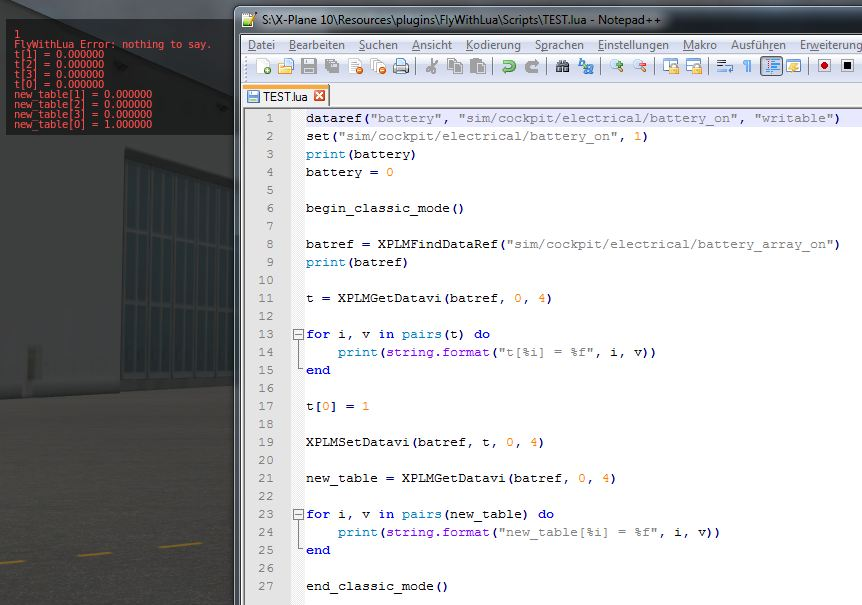
\includegraphics[width=12cm]{FWLclassic.jpg}

Forget the rest of the code and look at lines 8 to 25. They show how to handle an array DataRef by reading and manipulation the battery. (In the more modern versions of X-Plane there is in fact more than one battery! But most planes only interact with the first battery.)

As you can see in line 8, the following functions will read references instead of strings. It is not possible to write:

\verb|t = XPLMGetDatavi("sim/cockpit/electrical/battery_array_on", 0, 4)|

You will crash the simulator if you try it. To find the right argument, you first have to use \verb|XPLMFindDataRef()| - a very slow function. If you like performance, use it only as often as needed.

In line no. 9 you force Lua to print \verb|batref|, the variable holding the reference to the battery DataRef. Lua says >>\verb|FlyWithLua Error: nothing to say.|<< because a reference is stored as a userdata, and can not be converted into a string, so the automatic converter results in \verb|nil| and the \verb|print()| function can't print it.

\newpage
\subsection{Writing classic functions}

To give values back to X-Plane, use one of these functions:

\subsubsection{XPLMSetDatai( \emph{DataRef}, \emph{variable or value})}

\begin{enumerate}
	\item \emph{DataRef} = The reference(!) of the DataRef you want to write into.
	\item \emph{variable or value} = The lua variable, carrying the value you want to write, or a value directly.
\end{enumerate}

Use this for integer DataRefs.

\subsubsection{XPLMSetDataf( \emph{DataRef}, \emph{variable or value})}

\begin{enumerate}
	\item \emph{DataRef} = The reference(!) of the DataRef you want to write into.
	\item \emph{variable or value} = The lua variable, carrying the value you want to write, or a value directly.
\end{enumerate}

Use this for float DataRefs.

\subsubsection{XPLMSetDatad( \emph{DataRef}, \emph{variable or value})}

\begin{enumerate}
	\item \emph{DataRef} = The reference(!) of the DataRef you want to write into.
	\item \emph{variable or value} = The lua variable, carrying the value you want to write, or a value directly.
\end{enumerate}

Use this for double DataRefs.

\subsubsection{XPLMSetDatavi( \emph{DataRef}, \emph{table}, \emph{inIndex}, \emph{inMax} )}

\begin{enumerate}
	\item \emph{DataRef} = The reference(!) of the DataRef you want to write into.
	\item \emph{table} = The lua table, carrying the values you want to write, with correct indexes!
	\item \emph{inIndex} = The index where you want to start.
	\item \emph{inMax} = The number of values you want to access.
\end{enumerate}

Use this for integer array DataRefs.

\subsubsection{XPLMSetDatavf( \emph{DataRef}, \emph{table}, \emph{inIndex}, \emph{inMax} )}

\begin{enumerate}
	\item \emph{DataRef} = The reference(!) of the DataRef you want to write into.
	\item \emph{table} = The lua table, carrying the values you want to write, with correct indexes!
	\item \emph{inIndex} = The index where you want to start.
	\item \emph{inMax} = The number of values you want to access.
\end{enumerate}

Use this for float array DataRefs.


\section{The Lua way to access DataRefs}

Classic code can be fine and super fast, but it is hard to read (and write). And all the methods to access DataRefs we know until now aren't good Lua code. The classic approach comes from the SDK's C code, so it fakes C-style to Lua. The modern style fakes a PLC and transfers DataRefs to Lua variables. A clever code, but a little bit confusing when we want to access array DataRefs. And it consumes more CPU power.

\subsection{A magic metatable}

The Lua way of life is to use a metatable. Metatables are one of the primary features making Lua unique to other programming languages. FlyWithLua respects this of course, and provides a magic metatable \verb|DATAREF_META_TABLE|.

The magic metatable is defined in the file FlyWithLua.ini:

\begin{lstlisting}[firstnumber=42]
-- create a magic metatable
DATAREF_META_TABLE = {}
DATAREF_META_TABLE.__index = function(t, key) return peek(t.reference, t.reftype, key) end
DATAREF_META_TABLE.__newindex = function(t, key, value) poke(t.reference, t.reftype, key, value) end
\end{lstlisting}

There are two undocumented functions in this metatable, \verb|peek()| and \verb|poke()|. Don't care about them. You do not need these functions, if you want to write a Lua-style script.

More important is, how the metatable works. It expects two values, \verb|reference| and \verb|reftype| as elements of the table it is attached to.

Let's create an empty table, add the elements needed by the metatable and attach the metatable to the table. In this example, we will access the well known battery DataRef.

\begin{lstlisting}
battery = {}
battery.reference = XPLMFindDataRef( "sim/cockpit/electrical/battery_array_on" )
battery.reftype = XPLMGetDataRefTypes( battery.reference )
setmetatable( battery, DATAREF_META_TABLE )
\end{lstlisting}

Now we test the code (write through XSquawkBox's input line).

\verb|>print( battery[0] )|

Lua takes a look inside the table \verb|battery|, searching for an element indexed with 0. The table itself does not provide an element with this index.

Lua knows, that a metatable is attached to the table \verb|battery|, so it looks into the metatable for an element with the given index.

As there is no element \verb|DATAREF_META_TABLE[0]|, Lua looks for an element \verb|__index| inside the metatable. An element \verb|__index| can be found as a function, and Lua now calls it this way:

\verb|DATAREF_META_TABLE.__index( battery, 0 )|

And the function finally returns:

\verb|peek( battery.reference, battery.reftype, 0 )|

This is resolved to 0, if the first battery is off, or to 1 if it is on.

Because of \verb|peek()| and \verb|poke()| ignoring the index, if the DataRef points to a single value instead of an array, you can do the same magic access with all DataRefs X-Plane provides. The only circumstance is to give a dummy index of 0 (zero) to all non-array DataRefs.

And if you give an index to a string DataRef, it will begin with the character at the index position (starting at position 0, not 1).

As \verb|peek()| and \verb|poke()| are C-style functions, all indexes will start at 0 (zero), not 1 (like Lua starts array indexes). This behavior was implemented, because of X-Plane's DataRefs will always use 0 for the first index.

To shorten the code, FlyWithLua provides a function to declare a magic table in one single line of code:

\subsubsection{\emph{table} = dataref\_table( \emph{DataRef} )}

\begin{enumerate}
	\item \emph{table} = The lua table, you want to contain your magic.
	\item \emph{DataRef} = The name of the DataRef as a string.
\end{enumerate}

Creating a new magic table to access the given DataRef, auto detecting the type of the DataRef.

\vspace{2ex}

\textbf{The function dataref\_table() initializes a direct access to the DataRef. This causes a conflict to the PLC\footnote{See section >>Understanding PLCs<< for more info.} behavior of FlyWithLua. As a consequence dataref\_table() always forces the script to be classic code.}

\textbf{Never use dataref() and dataref\_table() together in the same script file!}

\newpage
\section{Manage your joysticks}

FlyWithLua was made to replace the plugin \verb|Button2DataRef|, a very popular plugin to manage your button and axis assignments. You can completely replace it with FlyWithLua 2.0.

This section of the quick manual will show a step-by-step creating process of a joystick config script.

\subsection{Get a basic configuration}

The first step is to load your most used plane into the simulator, click into the joystick configuration menu of X-Plane, and setup everything as you want it to be.

Then restart X-Plane (with the same plane). Every time X-Plane is shut down, it saves your last settings in a preference file:

\emph{<<place where you store the sim>>}\verb|/X-Plane 10/Output/preferences/X-Plane.prf|

This file keeps all joystick settings for the next run in a non Lua friendly way:

\begin{lstlisting}[firstnumber=1680]
...
_joy_AXIS_use97 0
_joy_AXIS_use98 0
_joy_AXIS_use99 0
_joy_BUTN_use0 sim/autopilot/fdir_on
_joy_BUTN_use1 sim/none/none
_joy_BUTN_use2 sim/view/chase
_joy_BUTN_use3 sim/view/chase
_joy_BUTN_use4 sim/general/zoom_in_fast
_joy_BUTN_use5 sim/general/zoom_out_fast
_joy_BUTN_use6 sim/none/none
...
\end{lstlisting}


You could copy\&paste the values out of this code, but there is an easier way. FlyWithLua translates X-Plane's preferences saved inside the \verb|X-Plane.prf| file into a Lua readable script code. The code is written to a file named:

\emph{<<sim storage>>}\verb|/X-Plane 10/Resources/plugins/FlyWithLua/initial_assingments.txt|

And yes, it's a >>\verb|txt|<< file, not a script file, because it is made for copy\&paste only.

You will find the lines above translated into:

\begin{lstlisting}[firstnumber=12]
...
clear_all_button_assignments()
set_button_assignment( (0*40) + 0, "sim/autopilot/fdir_on" )
set_button_assignment( (0*40) + 2, "sim/view/chase" )
set_button_assignment( (0*40) + 3, "sim/view/chase" )
set_button_assignment( (0*40) + 4, "sim/general/zoom_in_fast" )
set_button_assignment( (0*40) + 5, "sim/general/zoom_out_fast" )
...
\end{lstlisting}

FlyWithLua ignores all lines defining axis or buttons to nothing. This is done by the two function calls \verb|clear_all_axis_assignments()| (in line 5) and \verb|clear_all_button_assignments()|.

This prevents you from coding 1600 button assignments and 100 axis assignments.

Write a new script file into the \verb|Scripts| folder and fill it with a copy of the automatic generated configuration code.

\subsection{Define your sticks}

As you can see, FlyWithLua has made all button numbers to mathematic exercises. Why that? You can easily see that all your joysticks start with it's first button numbered by a multiple of 40. FlyWithLua prepared the code to use a nice standard function of text editors: >>replace<<.

Go to the beginning of your configuration script and type in a line like this:

\verb|LeftHandSteeringStick = 0|

Then use your editor to replace all >>\verb|(0*40)|<< with >>\verb|LeftHandSteeringStick|<<.

The result will look similar to this code:

\begin{lstlisting}[firstnumber=12]
...
LeftHandSteeringStick = 0

clear_all_button_assignments()
set_button_assignment( LeftHandSteeringStick + 0, "sim/autopilot/fdir_on" )
set_button_assignment( LeftHandSteeringStick + 2, "sim/view/chase" )
set_button_assignment( LeftHandSteeringStick + 3, "sim/view/chase" )
set_button_assignment( LeftHandSteeringStick + 4, "sim/general/zoom_in_fast" )
set_button_assignment( LeftHandSteeringStick + 5, "sim/general/zoom_out_fast" )
...
\end{lstlisting}

Now you are prepared to buy a new USB device. If your stick in your left hand starts at button number 160 after you plug in an other joystick device, you will only have to change one line in your code (line 13 in the example above). This is very cool if you are tired of still reconfiguring your setup, while all the other members of the LAN party starts flying.

\subsection{Define type specific assignments}

Next step is to define settings, where plane types other than your favorite one need to be reconfigured. If your most used plane is a C172, and you want to fly the MD902 Explorer and a Bell 206 too, define a >>helicopter class<<.

The helicopter needs all >>little helpers<< like nullzone, sensitivity or augment at value 0.0 - to give maximum control into your hand.

And of course the throttle has to be replaced by a collective.

\begin{lstlisting}[firstnumber=134]
-- all helicopter will get a unique setting as default
function set_helicopter_assignments()
    set_axis_assignment(12, "collective", "normal")
    set( "sim/joystick/joystick_pitch_nullzone",       0.0 )
    set( "sim/joystick/joystick_roll_nullzone",        0.0 )
    set( "sim/joystick/joystick_heading_nullzone",     0.0 )
    set( "sim/joystick/joystick_pitch_augment",        0.0 )
    set( "sim/joystick/joystick_roll_augment",         0.0 )
    set( "sim/joystick/joystick_heading_augment",      0.0 )
    set( "sim/joystick/joystick_pitch_sensitivity",    0.0 )
    set( "sim/joystick/joystick_roll_sensitivity",     0.0 )
    set( "sim/joystick/joystick_heading_sensitivity",  0.0 )
end
\end{lstlisting}

After these lines of code, you can bind individual Helicopters (or Planes) to your aircraft types:

\begin{lstlisting}[firstnumber=156]
-- MD902 Explorer (EXPL)
if PLANE_ICAO == "EXPL" then
    set_helicopter_assignments()
end

-- Bell 206 Dreamfoil
if PLANE_ICAO == "B06" then
    set_helicopter_assignments()
end
\end{lstlisting}

If a plane has no ICAO code, go into the Planemaker and correct it. Or you can use the predefined variable \verb|PLANE_TAILNUMBER| instead of \verb|PLANE_ICAO|, if it is unique to this individual aircraft.

The work has to be done manually, there is no automatic way to define classes and bind aircrafts to them. But it is easy to copy some lines and change the values. If you redefine a button command, use the >>button advanced<< menu of X-Plane. You can copy\&paste the command string.

Finish!

From now on you will always start with the right setting in all aircrafts you cover by your script.

\subsection{Lua for cockpit builders}

If you build a home cockpit like with Button2DataRef, you may want to bind buttons to DataRefs. This is different to handle, if you are used to write B2D code, but not too complex.

FlyWithLua offers two functions, \verb|button()| and \verb|last_button()|. The function \verb|button()| needs the number of the button as its argument and delivers \verb|true| if the button is pressed, else you get \verb|false| returned. The function \verb|last_buuton()| gives the state one frame ago.

Let's compare some code. First you get the old Button2DataRef code, followed by the Lua code, doing exactly the same.

This is a typical configuration of a switch firing into a joystick button. If it is pressed (on), the battery should be on, else it should be set to off:

\verb|#IF BUTTON 13 SWITCHES FROM 1 TO 1 SET sim/cockpit/electrical/battery_on TO 1|
\verb|#IF BUTTON 13 SWITCHES FROM 0 TO 0 SET sim/cockpit/electrical/battery_on TO 0|
\begin{lstlisting}
if button(13) then
   set( "sim/cockpit/electrical/battery_on", 1 )
else
   set( "sim/cockpit/electrical/battery_on", 0 )
end
\end{lstlisting}

Next we want to release the parking brake if button 166 is released:

\verb|#IF BUTTON 166 SWITCHES FROM 1 TO 0 SET sim/flightmodel/controls/parkbrake TO 0|
\begin{lstlisting}
if not button(166) and last_button(166) then
   set( "sim/flightmodel/controls/parkbrake", 0 )
end
\end{lstlisting}

Remember to put all your >>button code<< into a function called every frame. This can be done in this way:

\begin{lstlisting}
function parkbrake_button()
   if not button(166) and last_button(166) then
      set( "sim/flightmodel/controls/parkbrake", 0 )
   end
end

do_every_frame( "parkbrake_button()" )
\end{lstlisting}

Or shorter by using the >>\verb|[[|<< and >>\verb|]]|<< string delimiters:

\begin{lstlisting}
do_every_frame( [[
if not button(166) and last_button(166) then
   set( "sim/flightmodel/controls/parkbrake", 0 )
end]] )
\end{lstlisting}

It will produce an useless empty line of code inside the \verb|do_every_frame()| routine, but this is not a performance issue, as Lua will interpret a byte-code. The byte-code is compiled on the fly and does not contain empty lines or comments slowing down the interpreter.

The next bad thing different to Button2DataRef is, that the function \verb|set()| is much slower than \verb|SET| in B2D code. If you want the speed of Button2DataRef, define a DataRef first. A fast code looks like this:

\begin{lstlisting}
dataref( "xp_parkbrake", "sim/flightmodel/controls/parkbrake", "writable" )
do_every_frame( [[
if not button(166) and last_button(166) then
   xp_parkbrake = 0
end]] )
\end{lstlisting}

Developers first law: \emph{Good code can prevent your simulator becoming a flip-book}.

As a consequence never use \verb|set()|, \verb|set_array()| or \verb|get()| in code looping every frame.

\newpage
\section{Understanding PLCs}

A \href{http://en.wikipedia.org/wiki/Programmable_logic_controller}{programmable logic controller} will do his work in endless cycling steps. These steps will loop:

\begin{enumerate}
	\item Read input values.
	\item Do the calculations.
	\item Write the output values.
\end{enumerate}

The >>modern part<< of FlyWithLua works like a PLC. Let's have a look into an example file:

\begin{lstlisting}
dataref("xp_battery", "sim/cockpit/electrical/battery_on", "writable")
dataref("ro_battery", "sim/cockpit/electrical/battery_on")
xp_battery = 1
print(xp_battery)
print(ro_battery)
\end{lstlisting}

You will get a warning in \verb|Log.txt|, but the script will run. Turn off the battery and reload the script. You will get:

\verb|1|\\
\verb|0|

The first printed result is what we expect. The battery was turned on, so after this we get a value of \verb|1| when querying the actual value of the battery. But is it really the actual value of the battery? No, it is the actual value of the variable connected to the battery.

Remember the PLC steps. We are in the calculating step, and as a fact of this, the value isn't transfered from the variable \verb|xp_battery| to the DataRef \verb|"sim/cockpit/electrical/battery_on"| yet. If all calculations are finished, FlyWithLua (who is acting like a PLC) goes to the writing step, pushing all writable variable-DataRef bindings towards X-Plane. (After that it copies all DataRefs to there variables, independent of the writable or readonly state, and comes to the next calculation.)

So the second output is \verb|0| and not \verb|1|, as the variable \verb|ro_battery| was filled with \verb|0| one PLC step before (you turned off the battery before reloading the script).

If you do not >>think as a PLC does<<, you might get unexpected results from your own code.

There are three possible solution. The first is to learn to think like a PLC.

\newpage
But if you don't like PLCs logic, you can use the functions \verb|get()|, \verb|set()| and \verb|set_array()|. This is the second solution. Look at the screen shot some pages before. The program starts:

\begin{lstlisting}
dataref("battery", "sim/cockpit/electrical/battery_on", "writable")
set("sim/cockpit/electrical/battery_on", 1)
print(battery)
\end{lstlisting}

The result of this code is (reloading again with batteries off):

\verb|1|

Hey! Is this real? Didn't we say \verb|battery| was filled with the value of \verb|0| during the pulling step before calculation?

Sure, we can try it out by adding a line of code:

\begin{lstlisting}
dataref("battery", "sim/cockpit/electrical/battery_on", "writable")
print(battery)
set("sim/cockpit/electrical/battery_on", 1)
print(battery)
\end{lstlisting}

The output is now:

\verb|0|\\
\verb|1|

Strange! The reason to this behavior is, that \verb|set()| will freeze the calculation, force a push step, does its own manipulation, forces a pull step and gets back to the calculation point, where it freezes the code. This doesn't even sounds complicated, it is enormous time consuming. So if you are a friend of performance, use \verb|set()| only in time-uncritical situations.

The same behavior is shown by \verb|get()| and \verb|set_array()|.

Coming to the third solution to escape from PLC logic. You can write classic mode script files. If you do all the XPLM voodoo on your own, everything goes directly from or to the simulator. But you will have to handle references and types. And you will get no error handling from FlyWithLua.

To be able to handle all three coding styles in a wildly mix of multiple script files, FlyWithLua needs two functions to switch his mode, \verb|begin_classic_mode()| and \verb|end_classic_mode()|.

Please do not care about these two functions in your scripts. Just write script files who use only one mode, a style mix of \verb|dataref()| and \verb|get()|/\verb|set()| (modern mode), or clean XPLM based code (classic mode). FlyWithLua will automatically insert the functions to change the mode if needed. You may check this by writing a debug file to disk.

As switching between modes will consume CPU, sort your scripts. You can start all modern style scripts with an uppercase letter and all classic style scripts with a lowercase letter. This will force only one switch, the minimum if you use both styles. Or name scripts written in one style like a lock and key service in a telephone directory (>>\verb|AAAAAA_my_lttle_script.lua|<<).

\section{Basic knowledge about DataRefs}

If you are unfamiliar to DataRefs, you should read this section, if you already know everything about DataRefs, you can skip it.

DataRefs are the main connection to X-Plane's bowels. Most of them are writable, giving you an enormous feature to tweak the simulator. But you need to know how they work and how to access them.

\subsection{What are DataRefs?}

As your Lua scripts uses global variables, X-Plane itself has it's own >>variables<<. But plugins can't see them, as they are not published to the plugins in a direct way. The plugin SDK/API offers C/C++ code to access the >>inner heart<< of X-Plane by DataRefs.

\vspace{2ex}

\textbf{Definition:} A DataRef is a reference to a place in memory, where X-Plane stores a special value. Each DataRef consists of a >>folder/file-type<< string giving the DataRef it's \textbf{name} and the \textbf{reference} itself.

\vspace{2ex}

\subsection{Find the right DataRefs}

If you want to find a DataRef to be used by your script, first take a look onto this site:

\url{http://www.xsquawkbox.net/xpsdk/docs/DataRefs.html}

This is the official website representing all DataRefs X-Plane offers. Always check this site and use the search function of your web browser to look out for a good DataRef to use.

If you found an useful DataRef, do not stop your search. Sometimes there are more than one DataRefs pointing to the same (logical) value. For example there is a DataRef >>\verb|sim/cockpit/| \verb|electrical/battery_on|<<. This DataRefs allows you to turn on/off the battery. But there is another DataRef >>\verb|sim/cockpit/electrical/battery_array_on|<<.

The first DataRef only points to the first battery of the aircraft, but the second DataRef points to an array of up to eight batteries. Most aircrafts will only simulate one battery, so it's enough to control it by the first DataRef. If an aircraft uses more than one battery, your script may result in mysterious behavior.

Take a look onto the columns of the official DataRef website. The third column shown in what version of X-Plane the DataRef is present. If you look onto the example above, you can see that all planes since X-Plane 6.60 will provide access to only one main battery, but since version 8.20 there are up to eight batteries.

If you read out the value behind >>\verb|sim/cockpit/misc/has_radar|<< using X-Plane 9.70, and you send it to a friend using X-Plane 10.10r3, he might be surprised by the beauty of your code.

\subsection{Accessing DataRefs}

A very important issue is, that the value in memory the DataRef points to, has a special byte structure. The DataRef itself only points to the first byte, no matter what structure (or length) the value has. It is your part to access the value the right way.

You can see the byte structure in the second column of the official DataRef list. If you find only \verb|int|, \verb|float| or \verb|double|, it is a single value behind the DataRef. If there are brackets behind the type, it is an array of this type.

Only look into the second column to examine the type, not in the name of the DataRef. For example >>\verb|sim/cockpit/electrical/battery_array_on|<< is an array of eight integer values, but >>\verb|sim/weather/cloud_type[2]|<< is only one single integer value, not an array of 2 values.

If you want access to a DataRef, you will first have to find out the reference. Use the function \verb|XPLMFindDataRef()| to get the reference. For example:

\verb|battery_ref = XPLMFindDataRef("sim/cockpit/electrical/battery_array_on")|

Now you have the reference address stored in a variable named \verb|battery_ref|. If you want to turn on the third battery, you must access the value stored behind the DataRef like this:

\begin{lstlisting}
-- find out the reference
battery_ref = XPLMFindDataRef("sim/cockpit/electrical/battery_array_on")

-- fill a table with the values from the DataRef
battery_array = XPLMGetDatavi(battery_ref, 0, 8)

-- change the value representing the third battery
battery_array[2] = 1

-- write the values back to X-Plane
XPLMSetDatavi(battery_ref, battery_array, 0, 8)
\end{lstlisting}

In this code, you change \verb|battery_array[2]| to turn on the third battery. All of X-Plane's arrays start at level 0 (like C/C++ does), not level 1 (like Lua does). The last value is \verb|battery_array[7]|. In the functions \verb|XPLMGetDatavi()| and \verb|XPLMSetDatavi()| your arguments are >>0, 8<<, you start at position 0 and get/set 8 values.

You can get all batteries into one table, do your changes to them, and at the last step write them all back to X-Plane. Between getting and setting the values can be as much of code as you like. But you do not need to get/set them all. If you only want to access to the third value, write a code like this instead:

\begin{lstlisting}
-- find out the reference
battery_ref = XPLMFindDataRef("sim/cockpit/electrical/battery_array_on")

-- fill a table with the values from the DataRef
battery_array = XPLMGetDatavi(battery_ref, 2, 1)

-- change the value representing the third battery
battery_array[2] = 1

-- write the values back to X-Plane
XPLMSetDatavi(battery_ref, battery_array, 2, 1)
\end{lstlisting}

Keep in mind that you still use a table, even if you want to access a single value. If the DataRef points to an array, you must use the >>array-function<<.

If you use the modern code to access, FlyWithLua will always translate into single values. The same code written in modern style will look like this:

\begin{lstlisting}
-- define the connection to the third battery
dataref("third_battery_on", "sim/cockpit/electrical/battery_array_on", "writable", 2)

-- change the value of the third battery
third_battery_on = 1
\end{lstlisting}

The modern code style is shorter, but it is impossible to get/set complete arrays at once to/from a Lua table.

\subsection{Observe the DataRef}

You should observe the behavior of a DataRef with the tool \href{http://wiki.x-plane.com/DataRefEditor}{DataRef Editor}. Sometimes a DataRef (to be exact: the value behind it) will not behave as you aspect it.

Let's have an example. You want to turn on the carb heat if there is ice in the engine. Your code is this:

\begin{lstlisting}
dataref("carb_heat", "sim/cockpit2/engine/actuators/carb_heat_ratio", "writable", 0)
dataref("icing", "sim/flightmodel/engine/ENGN_crbice", "readonly")

function automatic_carb_heat()
   -- if carb is icing then switch heat on 
   if(icing == 1) then
      carb_heat = 1
   else
      carb_heat = 0
   end	
end
\end{lstlisting}

Everything seems to be fine, FlyWithLua didn't produce an error message and all other stuff works well. Only your function \verb|automatic_carb_heat()| will not react to ice inside the engine. Let's observe the value of \verb|sim/flightmodel/engine/ENGN_crbice| with the DataRef Editor.

Your code expects an integer value (yes = 1, no = 0), like the \verb|third_battery_on| in the example above. But \verb|sim/flightmodel/engine/ENGN_crbice| is an array of \verb|float| values, representing a ratio of icing. The values start at zero, but they will grow up slowly. Before they reach a value of \verb|1.0|, your plane usually crashed into ground.

If you absolutely dislike ice in your engine, change the code to:

\begin{lstlisting}
dataref("carb_heat", "sim/cockpit2/engine/actuators/carb_heat_ratio", "writable", 0)
dataref("icing", "sim/flightmodel/engine/ENGN_crbice", "readonly")

function automatic_carb_heat()
   -- if carb is icing then switch heat on 
   if(icing > 0) then
      carb_heat = 1
   else
      carb_heat = 0
   end
end
\end{lstlisting}

As the value for the carb heat is a ratio too, but you are firing all or nothing, you may be too power consuming. In times fuel gets more and more expansive, it might be better to give more power to the carb heat, if there is more ice in the engine. Let your fantasy create a nice mathematic model for the relationship level of ice ---> level of carb heat.

\begin{lstlisting}
dataref("carb_heat", "sim/cockpit2/engine/actuators/carb_heat_ratio", "writable", 0)
dataref("icing", "sim/flightmodel/engine/ENGN_crbice", "readonly")

function automatic_carb_heat()
   -- if carb is icing then switch heat on 
   if(icing > 0) then
      carb_heat = 0.25 + icing * 3/4
   else
      carb_heat = 0
   end
end
\end{lstlisting}

Now you are using all benefits of \verb|float| ratio values. The world is more than black/white, there are nearly\footnote{As a C/C++ float value is stored into a limited number of bytes, it represents a collection of discrete values.} unlimited shades of gray.

\newpage
\section{Take Lua into consideration}

There are some specials Lua offer, a script developer needs to know. In this section, we will show some common mistakes/problems in scripting. If you are familiar with Lua, skip this section.

We will write an example file, not included in the FlyWithLua package. To follow this text, turn on X-Plane and start a text editor. Then copy\&paste the examples and see how X-Plane reacts.

\subsection{Strings inside of strings}

Let's start with a typical script. You make a script printing out the solution of the universe.

\begin{lstlisting}
xyz = 42
do_every_draw("draw_string(50, 500, string.format("The solution is %i", xyz))")
\end{lstlisting}

The script seems to be ok, but FlyWithLua reacts like this (lines copied from Log.txt):

\begin{lstlisting}[firstnumber=1136]
FlyWithLua Info: Lua engine (re)started. LUA_RUN = 2, SDK_VERSION = 210, XPLANE_VERSION = 10101, XPLANE_LANGUAGE = German and XPLANE_HOSTID = 1
FlyWithLua: Load ini file.
FlyWithLua: Searching for Lua script files
FlyWithLua: Sorting Lua script files
FlyWithLua: Start loading script file Resources/plugins/FlyWithLua/Scripts/ALPHA.lua
FlyWithLua Info: No classic commands found inside the file.
FlyWithLua: Lua has crashed, can't execute script file: Resources/plugins/FlyWithLua/Scripts/ALPHA.lua
FlyWithLua: Error loading script file Resources/plugins/FlyWithLua/Scripts/ALPHA.lua
FlyWithLua Debug Info: The Lua stack contains the following elements:
Resources/plugins/FlyWithLua/Scripts/ALPHA.lua:2: ')' expected near 'The'
FlyWithLua Debug Info: Debug file written to "<<x-plane dir>>/FlyWithLua_Debug.txt".
\end{lstlisting}

Lua crashes! The reason is, that you put a string into a string the wrong way. The reason is not, that you forgot a closing bracket. Always think twice when reading an error message!

A string can be set between the char >>\verb|"|<< (double quotation), but you can also use >>\verb|'|<< (single quotation). This can set an inner string into an outer string.

The correct script looks like this:

\begin{lstlisting}
xyz = 42
do_every_draw('draw_string(50, 500, string.format("The solution is %i", xyz))')
\end{lstlisting}

Or you can write it this way:

\begin{lstlisting}
xyz = 42
do_every_draw("draw_string(50, 500, string.format('The solution is %i', xyz))")
\end{lstlisting}

\subsection{Multiple line strings}

If you want to declare a string over more than one line, you must use the delimiters >>\verb|[[|<< (at the beginning) and >>\verb|]]|<< (at the end). This can look like:

\begin{lstlisting}
xyz = 42
do_every_draw([[draw_string(50, 520, "This is all you need to know:")
draw_string(50, 500, string.format("The solution is %i", xyz))]])
\end{lstlisting}

There are a lot of more tricks handling strings. Please take a look into the \href{http://www.lua.org/manual/5.2/manual.html#3.1}{official Lua 5.2 manual}.

\subsection{Global or local variables?}

We will now name the script from above to \verb|ALPHA.lua| and write a second script named \verb|BETA.lua|:

\begin{lstlisting}
xyz = 17

function beta_print_xyz()
    draw_string(50, 450, string.format("BETA: xyz = %i", xyz))
end

do_every_draw("beta_print_xyz()")
\end{lstlisting}

This will produce no error message, all scripts run as they should, but the solution is now 17.

Why? It is because the first line of \verb|BETA.lua| will overwrite variable \verb|xyz| first initialized in line 1 of script \verb|ALPHA.lua| (all scripts are compiled in alphabetical order). All variables used in Lua are global variables, and every code can see and manipulate the variable!

But you can make a variable local. Make it local means, it can't be seen from code outside of the block it is declared in. To declare a local variable, just write >>\verb|local|<< in front of the first use of the variable. Change \verb|BETA.lua| to:

\begin{lstlisting}
local xyz = 17

function beta_print_xyz()
    draw_string(50, 450, string.format("BETA: xyz = %i", xyz))
end

do_every_draw("beta_print_xyz()")
\end{lstlisting}

Now the solution switches back to 42. What happened here? The first line of \verb|BETA.lua| declares a local variable \verb|xyz|. The global variable \verb|xyz| from script \verb|ALPHA.lua| still exists, but a local variable will hide a global variable with an identical name. All code inside the active block will now use the local variable instead of the global.

A function defined in the same block will now see the local variable \verb|xyz| of the code block made by the script file (a file is a block of code).

Now we know how clever a script can be written, we will change the code of \verb|ALPHA.lua| too. This will avoid conflicts with scripts using a global variable named \verb|xyz|, even if we do not have a script like this at the moment. But we could get one from a friend or download one from the Internet.

\begin{lstlisting}
local xyz = 42
do_every_draw([[draw_string(50, 520, "This is all you need to know:")
draw_string(50, 500, string.format("The solution is %i", xyz))]])
\end{lstlisting}

Crash!

Was it not clever to declare every variable as local? What happened now?

The reason is, that the command \verb|do_every_draw()| always creates a totally new block of code, containing all strings from all scripts in it. This block is completely independent to all other code you give to Lua. If you write a debug file, you can see this block inside the file \verb|FlyWithLua_debug.txt| in X-Plane's main directory.

The functions \verb|do_sometimes()|, \verb|do_often()| and \verb|do-every_frame()| behave the same way. \verb|add_macro()| creates two independent blocks of code and \verb|create_command()| creates three independent blocks of code, while \verb|add_ATC_macro()| creates only one.

The trick in \verb|BETA.lua| is, that we call a function \verb|beta_print_xyz()| from the \verb|do_every_draw()| command block. Lua jumps into the function \verb|beta_print_xyz()|. This is a jump into the block automatically created by the file \verb|BETA.lua|.

\textbf{Important info:} A jump from one block into another block (as made by a function call) changes the view onto the variables (if local variables are declared)!

\textbf{Conclusion:} If you want to write code that does not make unwanted side-effects to other scripts, keep all variables local and mask everything you want to be done continuously in a function.

\textbf{Next conclusion:} As the function \verb|DataRef()| always creates a global variable, you must write classic code, if you plan to share a script online. You will never know if the user, who downloaded your script, uses the same \verb|DataRef()| binding as your script does. As long as you are the only user of your script, you can do whatever you want. Just like in real life.

\subsection{Tables are tables}

If you use tables in Lua, you can't use the name of the table as a variable. This code will fail without a warning (it simply redefines the variable to hold a number instead of a table):

\begin{lstlisting}
local battery = dataref_table( "sim/cockpit/electrical/battery_on" )
battery = 1
\end{lstlisting}

If you want to turn on the battery, use this code:

\begin{lstlisting}
local battery = dataref_table( "sim/cockpit/electrical/battery_on" )
battery[0] = 1
\end{lstlisting}

\newpage
\section{FlyWithLua 2.7.x Added New Features}

Starting with version 2.7.0, FlyWithLua now supports creating native plugin windows. There are two ways to use them:

\hspace*{10mm}	graphics module: You can use the existing graphics module of FlyWithLua to draw into 
\hspace*{10mm}	the windows, see examples included in the "Scripts (disabled)" folder that start with
\hspace*{10mm}	"floating\_wnd".

\hspace*{10mm}	imgui: FlyWithLua now supports creating imgui GUIs. imgui is an awesome 3rd party
\hspace*{10mm}	GUI library that makes it really easy to create stunning GUIs. See the examples included
\hspace*{10mm}	in the "Scripts (disabled)" folder that start with "imgui".

Why would you want to use these new capabilities instead of using existing GUI libraries written in
lua?

\hspace*{10mm}	The windows can be moved and popped out to a native window

\hspace*{10mm}	The performance is better because the GUI isn't created by lua (for imgui windows)

\hspace*{10mm}	Imgui is more powerful than the existing libraries - for example, you can load an image
\hspace*{10mm}	file (even png and jpg) and use it as a background image or button or whatever...

\hspace*{10mm}	Both window types automatically (!) work in VR

Here are a few teasing images to see what is now possible.

\newpage
\begin{center}
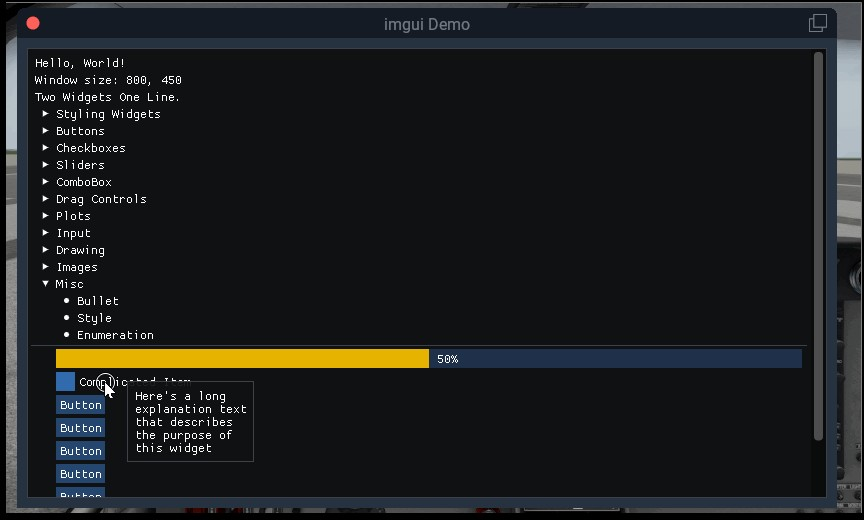
\includegraphics[width=10cm]{imgui_demo.jpg} 
\end{center}

\begin{center}
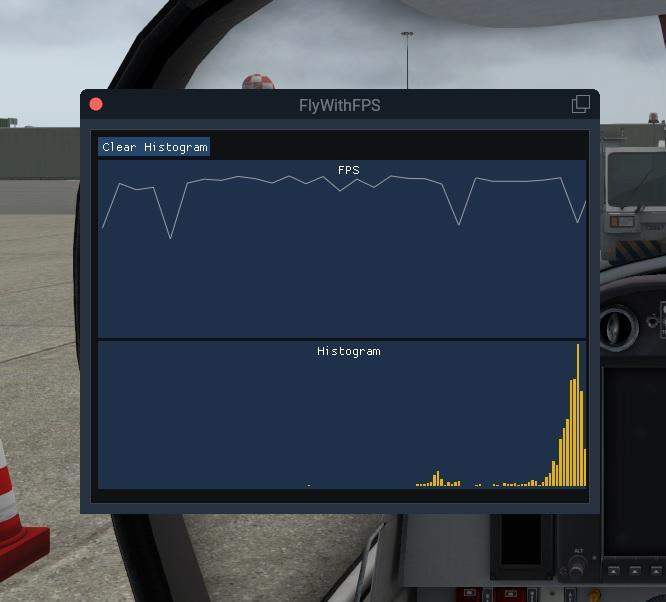
\includegraphics[width=10cm]{imgui_plots.jpg}
\end{center}

\newpage
\begin{center}
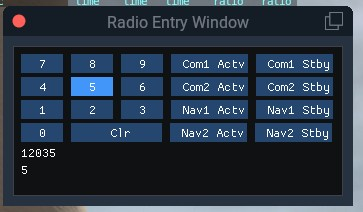
\includegraphics[width=10cm]{Radio_Entry_Window.jpg}
\end{center}

\begin{center}
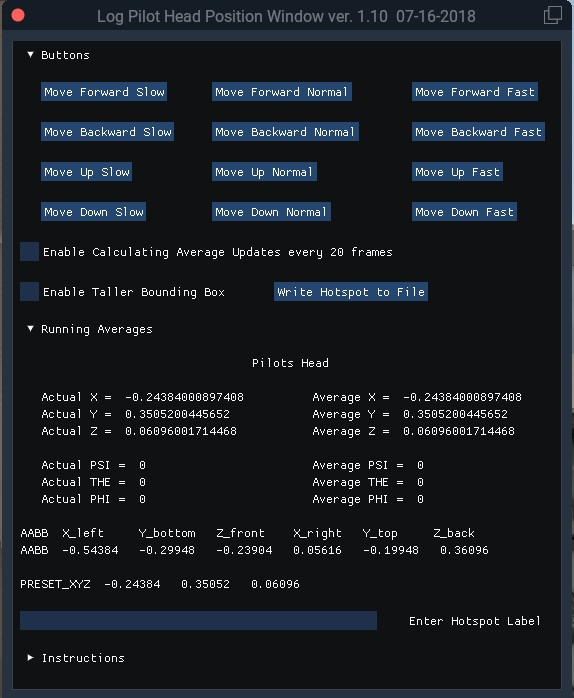
\includegraphics[width=10cm]{LogPilotHeadPosition.jpg}
\end{center}

\newpage
The following functions don't work with floating windows in VR anymore, no matter if using imgui or FWL: do\_every\_frame, do\_on\_mouse\_click.

Instead of using do\_every\_frame, you can register a drawing function that is called everytime X-Plane
draws the window. It gets passed the x and y coordinates of the window's lower left corner as absolute
coordinates. This is required because FWL's graphics functions take absolute screen coordinates and
you have to make sure that you actually draw into the window. For example, if you pass (0, 0) as
coordinates to a lua function that draws a dot, the pixel would always be in the lower left of
the screen because they are absolute coordinates. But if the window doesn't cover that part of the
screen, the pixel wouldn't be visible in the window. So if you want to put the pixel in the lower left of
the window, pass (x, y) as coordinates to the lua functions. If you want a button on top of the window
with a padding of 10px from the borders, you would draw a rectangle with the first point at (x + 10, y +
height - 10). I attached a sketch to visualize this. x and y are passed as paramters to your drawing
function by FlyWithLua and you must use them to place your pixels inside the window.

And instead of do\_on\_mouse\_click, you can register an onclick function with the floating window.
That function is only called if the click actually happened inside the window, so it gets passed relative
coordinates already. So if the user clicks on the upper left of your button's rectangle, it would get
passed (10, height - 10). You would then have to set a flag to remember that the user clicked
somewhere so that you can then check this variable the next time the window is drawn.

Using imgui, you don't need to care about drawing the controls yourself or mapping the clicks back to
the controls. In fact, you don't need to register an onclick function at all. imgui is an immediate GUI,
that means the controls don't have any internal state. You can't ask a checkbox if it is currently checked
and you can't set a callback function to a button. They just have no state at all. How does it work then?
For imgui windows, you register a builder function. That function is also called everytime the window
is drawn. If you want to place a button, you just call
imgui.Button("My Button")

When you do that, imgui does not only draw the button, it also checks if the mouse button was released
over this area in the last frame. And if that's the case, the Button function returns true! It's a little weird
to get used to in the beginning, but all imgui functions actually return boolean values to indicate
whether they were just being used. So if you want to react on the button, you just do something like
this:

if imgui.Button("My Button") then \newline
\hspace*{10mm}	command\_once("some x-plane command") \newline
end

In the next frame, the mouse will not have been released over this button again, so the button doesn't
return true in the next frame, resulting in your action being only called once as desired. The same goes
for other controls like sliders and checkboxes - they return a boolean to indicate if you need to react on
a change.

\newpage
\begin{center}
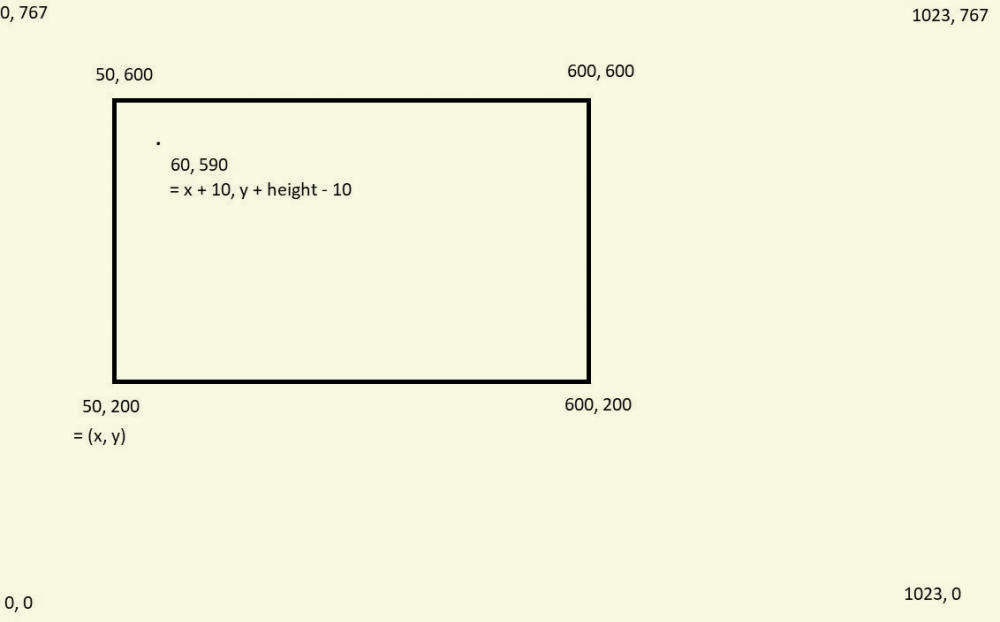
\includegraphics[width=15cm]{FlyWithLuaFloatingWindow.jpg}
\end{center}

\newpage
\section{Floating Windows}

Starting with version 2.7.0 NG we have floating windows that can be in 2d, popped out or in VR. They are X-Plane 11 Window API style windows that can be created with Lua. There are examples of these kind of windows in the "Scripts (disabled)" folder anf are prefaced with "floating\_wnd\_".

\subsection{\hspace*{1.0mm}demo\_floating\_wnd = float\_wnd\_create(800,450,1,false)}

This is how you create a floating windows in lua.

"demo\_floating\_wnd" is the name of the handle of the window that is created.

The first two parameters specify the size of the window in boxels. Boxels are scalable pixels.If the UI scale is set to 100\% in the settings, a boxel equals a pixel. However, if the user sets the UI scale to more than 100\%, a boxel will be scaled to span multiple pixels.

The third parameter specifies the window decoration. The following decorations are possible:
\hspace*{10mm}	0: "X-Plane will draw no decoration for your window, and apply no automatic click
\hspace*{10mm}	handlers. The window will not stop click from passing through its bounds. This is
\hspace*{10mm}	suitable for "windows" which request, say, the full screen bounds, then only draw in
\hspace*{10mm}	a small portion of the available area."

\hspace*{10mm}	1: "The default decoration for "native" windows, like the map. Provides a solid back-    \hspace*{10mm}  ground, as well as click handlers for resizing and dragging the window."

\hspace*{10mm}	2: "X-Plane will draw no decoration for your window, nor will it provide resize han-
\hspace*{10mm}	dlers for your window edges, but it will stop clicks from passing through your win-
\hspace*{10mm}	dows bounds."

\hspace*{10mm}	3: "Like 2, but with resizing; X-Plane will draw no decoration for your window, but
\hspace*{10mm}	it will stop clicks from passing through your windows bounds, and provide automatic
\hspace*{10mm}	mouse handlers for resizing."

The last parameter configures whether you want to use imgui for the floating window.
The return value is a handle to the window that can be used to configure additional things.

\subsection{\hspace*{1.0mm}float\_wnd\_set\_title(demo\_floating\_wnd, \ "floating window Demo")}

This function sets the title of the window if it has a decoration.

The first parameter must be a handle to the window previously created with the float\_wind\_create.

The second parameter is the title of the window.


\subsection{\hspace*{1.0mm}float\_wnd\_set\_position(demo\_floating\_wnd, 775, 650)}

This function sets the initial position of the window.

The first parameter must be a handle to a window previously created with float\_wnd\_create.

The second and third parameters set the initial position of the window.

\subsection{\hspace*{1.0mm}float\_wnd\_set\_ondraw(demo\_floating\_wnd, \ "on\_draw\_floating\_window")}

This function sets the name of the ondraw function.

The first parameter must be a handle to a window previously created with float\_wnd\_create.

The second parameter sets the name of the ondraw function.

\subsection{\hspace*{1.0mm}float\_wnd\_set\_onclick(demo\_floating\_wnd, "on\_click\_floating\_window")}

This function sets the name of the onclick function.

The first parameter must be a handle to a window previously created with float\_wnd\_create.

The second parameter sets the name of the onclick function.

\subsection{\hspace*{1.0mm}float\_wnd\_set\_onclose(demo\_floating\_wnd, "on\_close\_floating\_window")}

This function sets the name of the onclose function.

The first parameter must be a handle to a window previously created with float\_wnd\_create.

The second parameter sets the name of the onclose function.

\subsection{\hspace*{1.0mm}xplm\_wnd = float\_wnd\_get\_xplm\_handle(demo\_floating\_wnd)}

This function gets the xplm handle of the window created above to be used with ffi.

"xplm\_wnd" is the name of the xplm handle of the window that was created.

The first parameter must be a handle to a window previously created with float\_wnd\_create.

\subsection{\hspace*{1.0mm}function on\_draw\_floating\_window(demo\_floating\_wnd, x3, y3)}

The first parameter must be a handle to a window previously created with float\_wnd\_create.

x and y are the origin of the window, i.e. the lower left

x increases to the right, y increases to the top

\subsection{\hspace*{1.0mm}function\ on\_click\_floating\_window(demo\_floating\_wnd, x3, y3)}

The first parameter must be a handle to a window previously created with float\_wnd\_create.

x and y are relative from the origin of the window, i.e. the lower left

\subsection{\hspace*{1.0mm}function\ on\_close\_floating\_window(demo\_floating\_wnd)}

When on\_close it called, it is illegal to do anything with the wnd variable.

It is also not allowed to create new windows in on\_close!

The first parameter must be a handle to a window previously created with float\_wnd\_create.

\newpage
\subsection{\hspace*{1.0mm}is\_popped = float\_wnd\_is\_popped(fwl\_wnd)}

"is\_popped" is the name of the boolean to know if the created window is popped out.

The parameter must be a handle to a window previously created with float\_wnd\_create.

\subsection{\hspace*{1.0mm}is\_visible = float\_wnd\_get\_visible(fwl\_wnd)}

"is\_visable" is the name of the boolean to know if the created window is visable.

The parameter must be a handle to a window previously created with float\_wnd\_create.

\subsection{\hspace*{1.0mm}is\_front = float\_wnd\_is\_front(fwl\_wnd)}

"is\_front" is the name of the boolean to know if the created window is in front.

The parameter must be a handle to a window previously created with float\_wnd\_create.

\subsection{\hspace*{1.0mm}is\_vr = float\_wnd\_is\_vr(fwl\_wnd)}

"is\_vr" is the name of the boolean to know if the created window is in vr.

The parameter must be a handle to a window previously created with float\_wnd\_create.

\subsection{\hspace*{1.0mm}function float\_wnd\_bring\_to\_front(fwl\_wnd)}

The function brings the created window to the front.

The parameter must be a handle to a window previously created with float\_wnd\_create.

\subsection{\hspace*{1.0mm}function float\_wnd\_set\_resizing\_limits(fwl\_wnd, minWidth, minHeight, maxWidth, maxHeight)}

The function sets the resizing limits for the created window.

The first parameter must be a handle to a window previously created with float\_wnd\_create.

The second parameter sets the  minimum width for the created window.

The third parameter sets the  minimum height for the created window.

The forth parameter sets the maximum width for the created window.

The fifth paramter sets the maximum height for the created window.

\subsection{\hspace*{1.0mm}function float\_wnd\_set\_positioning\_mode(fwl\_wnd, 1, -1)}

This function sets the positioning mode of the created window.

The first parameter must be a handle to a window previously created with float\_wnd\_create.

The second parameter sets the policy for how X-Plane will position whe created window.

\hspace*{10mm}	Here are the aviable values for the policy.

\hspace*{10mm}	xplm\_WindowPositionFree \hspace*{23.0mm}	0\newline
\hspace*{10mm}	xplm\_WindowCenterOnMonitor \hspace*{15.0mm}	1\newline
\hspace*{10mm}	xplm\_WindowFullScreenOnMonitor \hspace*{8.5mm}	2\newline
\hspace*{10mm}	xplm\_WindowFullScreenOnAllMonitors \hspace*{2.5mm}	3\newline
\hspace*{10mm}	xplm\_WindowPopOut \hspace*{31.2mm}	4\newline
\hspace*{10mm}	xplm\_WindowVR \hspace*{38.0mm}	5

The thrid parameter is the monitor index.

\subsection{\hspace*{1.0mm}function float\_wnd\_set\_gravity(fwl\_wnd, gLeft, gTop, gRight, gBottom)}

A window's "gravity" controls how the window shifts as the whole X-Plane window resizes. A gravity of 1 means the window maintains its positioning relative to the right or top edges, 0 the left/bottom, and 0.5 keeps it centered.

Default gravity is (0, 1, 0, 1), meaning your window will maintain its position relative to the top left and will not change size as its containing window grows.

If you wanted, say, a window that sticks to the top of the screen (with a constant height), but which grows to take the full width of the window, you would pass (0, 1, 1, 1). Because your left and right edges would maintain their positioning relative to their respective edges of the screen, the whole width of your window would change with the X-Plane window.

Only applies to modern windows. (Windows created using the deprecated XPLMCreateWindow(), or windows compiled against a pre-XPLM300 version of the SDK will simply get the default gravity.) 


The first parameter must be a handle to a window previously created with float\_wnd\_create.

The remaining parameters follow the discription above.

\subsection{\hspace*{1.0mm}function float\_wnd\_set\_geometry(fwl\_wnd, nLeft, nTop, nRight, nBottom)}

This routine allows you to set the position and size of a normal 2d window.

\emph{for floating window, equivalent to - void XPLMSetWindowGeometry(XPLMWindowID inWindowID, int inLeft, int inTop, int inRight, int inBottom))}

The units and coordinate system match those of XPLMGetWindowGeometry(). That is, modern windows use global desktop boxel coordinates, while legacy windows use pixels relative to the main X-Plane display.

Note that this only applies to "floating" windows (that is, windows that are drawn within the X-Plane simulation windows, rather than being "popped out" into their own first-class operating system windows). To set the position of windows whose positioning mode is xplm\_WindowPopOut, you'll need to instead use XPLMSetWindowGeometryOS().

The first parameter must be a handle to a window previously created with float\_wnd\_create.

The remaining parameters set position and size of the created window.

\subsection{\hspace*{1.0mm}function float\_wnd\_set\_geometry(fwl\_wnd, pLeft, pTop, pRight, pBottom)}

This routine allows you to set the position and size of a poped out or OS 2d window.

\emph{for OS window, equivalent to       - void XPLMSetWindowGeometryOS(XPLMWindowID inWindowID, int inLeft, int inTop, int inRight, int inBottom)}

This routine allows you to set the position and size, in operating system pixel coordinates, of a popped out window (that is, a window whose positioning mode is xplm\_WindowPopOut, which exists outside the X-Plane simulation window, in its own first-class operating system window).

Note that you are responsible for ensuring both that your window is popped out (using XPLMWindowIsPoppedOut()) and that a monitor really exists at the OS coordinates you provide (using XPLMGetAllMonitorBoundsOS()).

The first parameter must be a handle to a window previously created with float\_wnd\_create.

The remaining parameters set position and size of the created window.

\newpage

\subsection{\hspace*{1.0mm}function float\_wnd\_set\_geometry(fwl\_wnd, vrWidth, vrHeight)}

This routine allows you to set the size of a VR window.

\emph{for VR window, equivalent to       - void XPLMSetWindowGeometryVR(XPLMWindowID inWindowID, int widthBoxels, int heightBoxels)}

This routine allows you to set the size, in boxels, of a window in VR (that is, a window whose positioning mode is xplm\_WindowVR).

Note that you are responsible for ensuring your window is in VR (using XPLMWindowIsInVR()).

The first parameter must be a handle to a window previously created with float\_wnd\_create.

The remaining parameters sets the size of the created window increasing or decreasing from a centered position.
 
\newpage

\subsection{\hspace*{1.0mm}nwinLeft, nwinTop, nwinRight, nwinBottom = float\_wnd\_get\_geometry(fwl\_wnd)}

This routine returns the position and size of a normal 2d window. The units and coordinate system vary depending on the type of window you have.

\emph{for floating window, equivalent to - void XPLMGetWindowGeometry(XPLMWindowID inWindowID, int * outLeft, int * outTop, int * outRight, int * outBottom)}

If this is a legacy window (one compiled against a pre-XPLM300 version of the SDK, or an XPLM300 window that was not created using XPLMCreateWindowEx()), the units are pixels relative to the main X-Plane display.

If, on the other hand, this is a new X-Plane 11-style window (compiled against the XPLM300 SDK and created using XPLMCreateWindowEx()), the units are global desktop boxels.

Pass NULL to not receive any paramter.

"nwinLeft" Name of variable for the left side of the created window.

"nwinTop" Name of variable for the top of the created window.

"nwinRight" Name of variable for the right side of the created window.

"nwinBottom" Name of variable for the bottom of the created window.

The first parameter must be a handle to a window previously created with float\_wnd\_create.

\newpage

\subsection{\hspace*{1.0mm}pwinLeft, pwinTop, pwinRight, pwinBottom = float\_wnd\_get\_geometry(fwl\_wnd)}

This routine returns the position and size of a poped out or OS window. The units and coordinate system vary depending on the type of window you have.

\emph{ for OS window, equivalent to       - void XPLMGetWindowGeometryOS(XPLMWindowID inWindowID, int * outLeft, int * outTop, int * outRight, int * outBottom)}

This routine allows you to set the position and size, in operating system pixel coordinates, of a popped out window (that is, a window whose positioning mode is xplm\_WindowPopOut, which exists outside the X-Plane simulation window, in its own first-class operating system window).

Note that you are responsible for ensuring both that your window is popped out (using XPLMWindowIsPoppedOut()) and that a monitor really exists at the OS coordinates you provide (using XPLMGetAllMonitorBoundsOS()).

"pwinLeft" Name of variable for the left side of the created window.

"pwinTop" Name of variable for the top of the created window.

"pwinRight" Name of variable for the right side of the created window.

"pwinBottom" Name of variable for the bottom of the created window.

The first parameter must be a handle to a window previously created with float\_wnd\_create.



\subsection{\hspace*{1.0mm}vrwinWidth, vrwinHeight = float\_wnd\_get\_geometry(fwl\_wnd)}

This routine returns the size of a VR window.

\emph{ for VR window, equivalent to       - void XPLMGetWindowGeometryVR(XPLMWindowID inWindowID, int * outWidthBoxels, int * outHeightBoxels)}

Returns the width and height, in boxels, of a window in VR. Note that you are responsible for ensuring your window is in VR (using XPLMWindowIsInVR()).

"vrWidth" Name of variable to set vr width of the created window.

"vrHeight" Name of variable to set vr height of the created window.

The first parameter must be a handle to a window previously created with float\_wnd\_create.

\newpage

\subsection{\hspace*{1.0mm}msgx, msgy = XPLMGetMouseLocationGlobal()}

Returns the current mouse location in global desktop boxels. Unlike XPLMGetMouseLocation(), the bottom left of the main X-Plane window is not guaranteed to be (0, 0)---instead, the origin is the lower left of the entire global desktop space. In addition, this routine gives the real mouse location when the mouse goes to X-Plane windows other than the primary display. Thus, it can be used with both pop-out windows and secondary monitors.

This is the mouse location function to use with modern windows (i.e., those created by XPLMCreateWindowEx()).

Pass NULL to not receive info about either parameter.

"msgx" Name of variable to get global x mouse location of the created window.

"msgy" Name of variable to get global y mouse location of the created window.

\subsection{\hspace*{1.0mm}ssWidth, ssHeight = XPLMGetScreenSize()}

This routine returns the size of the main X-Plane OpenGL window in pixels. This number can be used to get a rough idea of the amount of detail the user will be able to see when drawing in 3-d.

"ssWidth" Name of variable to get screen size width.

"ssHeight" Name of variable to get screen size height.

\newpage

\subsection{\hspace*{1.0mm}bLeft, bTop, bRight, bBottom = XPLMGetScreenBoundsGlobal()}

This routine returns the bounds of the "global" X-Plane desktop, in boxels. Unlike the non-global version XPLMGetScreenSize(), this is multi-monitor aware. There are three primary consequences of multimonitor awareness.

First, if the user is running X-Plane in full-screen on two or more monitors (typically configured using one full-screen window per monitor), the global desktop will be sized to include all X-Plane windows.

Second, the origin of the screen coordinates is not guaranteed to be (0, 0). Suppose the user has two displays side-by-side, both running at 1080p. Suppose further that they've configured their OS to make the left display their "primary" monitor, and that X-Plane is running in full-screen on their right monitor only. In this case, the global desktop bounds would be the rectangle from (1920, 0) to (3840, 1080). If the user later asked X-Plane to draw on their primary monitor as well, the bounds would change to (0, 0) to (3840, 1080).

Finally, if the usable area of the virtual desktop is not a perfect rectangle (for instance, because the monitors have different resolutions or because one monitor is configured in the operating system to be above and to the right of the other), the global desktop will include any wasted space. Thus, if you have two 1080p monitors, and monitor 2 is configured to have its bottom left touch monitor 1's upper right, your global desktop area would be the rectangle from (0, 0) to (3840, 2160).

Note that popped-out windows (windows drawn in their own operating system windows, rather than "floating" within X-Plane) are not included in these bounds.

"bLeft" Name of variable for the left bounds of the "global" X-Plane desktop, in boxels.

"bTop" Name of variable for the top bounds of the "global" X-Plane desktop, in boxels.

"bRight" Name of variable for the right bounds of the "global" X-Plane desktop, in boxels.

"bBottom" Name of variable for the bottom bounds of the "global" X-Plane desktop, in boxels.

\newpage

\subsection{\hspace*{1.0mm}tOS = XPLMGetAllMonitorBoundsOS()}

This routine immediately calls you back with the bounds (in pixels) of each monitor within the operating system's global desktop space. Note that unlike XPLMGetAllMonitorBoundsGlobal(), this may include monitors that have no X-Plane window on them.

Note that this function's monitor indices match those provided by XPLMGetAllMonitorBoundsGlobal(), but the coordinates are different (since the X-Plane global desktop may not match the operating system's global desktop, and one X-Plane boxel may be larger than one pixel).

This function returns the following values in a lua multi-dimensional table (an element for each monitor):

    int        MonitorIndex;
    int        inLeft;
    int        inTop;
    int        inRight;
    int        inBottom;
 

To access the values in FWL, use the following format: tOS[x].yyyy, where x = monitor number, and yyyy is table member.

Example for monitor 1: tOS[1].inLeft; tOS[1].inBottom; monitor 2: tOS[2].inLeft; tOS[2].inBottom 

\subsection{\hspace*{1.0mm}tGB = XPLMGetAllMonitorBoundsGlobal()}

This routine immediately calls you back with the bounds (in boxels) of each full-screen X-Plane window within the X-Plane global desktop space. Note that if a monitor is *not* covered by an X-Plane window, you cannot get its bounds this way. Likewise, monitors with only an X-Plane window (not in full-screen mode) will not be included.

If X-Plane is running in full-screen and your monitors are of the same size and configured contiguously in the OS, then the combined global bounds of all full-screen monitors will match the total global desktop bounds, as returned by XPLMGetScreenBoundsGlobal(). (Of course, if X-Plane is running in windowed mode, this will not be the case. Likewise, if you have differently sized monitors, the global desktop space will include wasted space.)

Note that this function's monitor indices match those provided by XPLMGetAllMonitorBoundsOS(), but the coordinates are different (since the X-Plane global desktop may not match the operating system's global desktop, and one X-Plane boxel may be larger than one pixel due to 150\% or 200\% scaling).

This function returns the following values in a lua multi-dimensional table (an element for each monitor):

    int        MonitorIndex;
    int        inLeft;
    int        inTop;
    int        inRight;
    int        inBottom;
 

To access the values in FWL, use the following format: tOS[x].yyyy, where x = monitor number, and yyyy is table member.

Example for monitor 1: tOS[1].inLeft; tOS[1].inBottom; monitor 2: tOS[2].inLeft; tOS[2].inBottom  

\newpage
\section{Imgui Windows}

Starting with version 2.7.0 NG we have imgui windows that can be in 2d, popped out or in VR. They are X-Plane 11 Window API style windows that use imgui widgets and can be created with Lua. There are examples of these kind of windows in the "Scripts (disabled)" folder and are prefaced with "imgui\_".

\subsection{demo\_wnd = float\_wnd\_create(800, 450, 1, true)}

The first two parameters specify the size of the window in boxels. Boxels are
scalable pixes. If the UI scale is set to 100\% in the settings, a boxel equals
a pixel. However, if the user sets the UI scale to more than 100\%, a boxel will
be scaled to span multiple pixels.

The third parameter specifies the window decoration. The following decorations are possible:
\hspace*{10mm}	0: "X-Plane will draw no decoration for your window, and apply no automatic click
\hspace*{10mm}	handlers. The window will not stop click from passing through its bounds. This is
\hspace*{10mm}	suitable for "windows" which request, say, the full screen bounds, then only draw in a
\hspace*{10mm}	small portion of the available area."

\hspace*{10mm}	1: "The default decoration for "native" windows, like the map. Provides a solid back-
\hspace*{10mm}	ground, as well as click handlers for resizing and dragging the window."

\hspace*{10mm}	2: "X-Plane will draw no decoration for your window, nor will it provide resize han-
\hspace*{10mm}	dlers for your window edges, but it will stop clicks from passing through your windows
\hspace*{10mm}	bounds."

\hspace*{10mm}	3: "Like 2, but with resizing; X-Plane will draw no decoration for your window, but
\hspace*{10mm}	it will stop clicks from passing through your windows bounds, and provide automatic
\hspace*{10mm}	mouse handlers for resizing."

The last parameter configures whether you want to use imgui for the floating window.

The return value is a handle to the window that can be used to configure additional things.

\subsection{float\_wnd\_set\_title(demo\_wnd, "Demo Window")}

This function sets the title of the window if it has a decoration.

The first parameter must be a handle to a window previously created with float\_wnd\_create.

The second parameter is the title of the window.

\subsection{float\_wnd\_set\_position(demo\_wnd, 775, 650)}

This function sets the initial position of the window.

The first parameter must be a handle to a window previously created with float\_wnd\_create.

The second and third parameters set the initial position of the window.

\subsection{float\_wnd\_set\_imgui\_builder(demo\_wnd, "build\_demo")}

imgui GUIs are built each frame. You will need to supply a function that is called every frame.

The first parameter must be a handle to a window previously created with float\_wnd\_create.

The second parameter must be the name of a function. Note that unlike other function in FlyWithLua, you
can only pass the name of a function here, not an arbitrary lua string. This function will be called for
every frame while the window is visible, so you don't need an additional do\_every\_frame unless you
also need to do things while the window is closed.

\subsection{float\_wnd\_set\_onclose(demo\_wnd, "closed\_demo")}

If the window has a decoration with a close button (like decoration 1), you might need a way to know when the users closes the window. This function can be used to setup a function to be called when the user closes the window.

The first parameter must be a handle to a window previously created with float\_wnd\_create and the second parameter must be the name of a function. Note that unlike other function in FlyWithLua, you
can only pass the name of a function here, not an arbitrary lua string. This function will be called
when the user closes the window. After the window is closed, its builder function will not be called
again and it is illegal to use the window handle variable returned by float\_wnd\_create, e.g. it is illegal
to set the window title after it was closed.

\newpage

\subsection{image\_id = float\_wnd\_load\_image(SCRIPT\_DIRECTORY .. "/imgui\_demo.jpg")}

imgui supports drawing images, so let's load one. The images must always be loaded globally to make sure they are only loaded once per script!

imgui widgets have no state, that means we need to store states of checkboxes, radio buttons etc. globally.

makeRed = false
\newline
sliderVal = 0
\newline
choice = 1
\newline
angle = 0
\newline
text = ""

\subsection{function build\_demo(wnd, x, y)}

This function is called for every frame. Use this function to create your GUI. The first parameter (wnd)
is the handle of the window. It is the same handle as the one returned by float\_wnd\_create. It is required if you have multiple windows that use the same builder function so you know which of these windows is currently being built. The x and y parameters are the current position of the window in OpenGL coordinates, i.e. the position of the lower left corner in global screen coordinates. These coordinates are only needed for using the graphics module on top of the imgui GUI. If you only use imgui, these coordinates are not required because imgui has its own coordinate system inside the window.

\subsection{function closed\_demo(wnd)}

This function is called when the user closes the window. Drawing or calling imgui functions is not allowed in this function as the window is already destroyed.


\newpage
\section{Debugging}

To domesticate the beast is a hard job sometimes. If you are searching an error inside your code, FlyWithLua gives you a nice little weapon. Just click the menu entry \verb|Write Debug file|. It writes a file \verb|FlyWithLua_debug.txt| into X-Plane's main directory. You may observe the file with a text editor able to recognize changes.

Inside the file you will find the content of Lua's stack, the list of DataRefs handled by the plugin and the content of the internal tables used by the plugin.

The debug info will show all global variables too. They are shown as name plus value. The debug info ends with a list of all global tables and functions. A lot of information to dive deep into FlyWithLua's bowels.

If this is still not enough, and you need to look into a local variable or need a continuous observation of a variable, write a debug code like this (debugging the example one section before):

\begin{lstlisting}
dataref("carb_heat", "sim/cockpit2/engine/actuators/carb_heat_ratio", "writable", 0)
dataref("icing", "sim/flightmodel/engine/ENGN_crbice", "readonly")

function automatic_carb_heat()
   -- debug the variable
   my_debug_string = string.format("before: icing = %f, carb_heat = %f", icing, carb_heat)

   -- if carb is icing then switch heat on 
   if(icing == 1) then
      carb_heat = 1
   else
      carb_heat = 0
   end	
   my_debug_string = my_debug_string .. string.format(" ==> after: icing = %f, carb_heat = %f", icing, carb_heat)
end

do_often("automatic_carb_heat()")

do_every_draw("if my_debug_string then draw_string(20, 20, my_debug_string) end")\end{lstlisting}

This example is pretty overobserved, but it shows how to observe more than one variable more than one time.

Please recognize the code in line 19. If you do not use the \verb|if| statement, FlyWithLua will crash, when the first drawing frame has nothing to draw. If you don't like the \verb|if| statement in the last line, start the script with:

\verb|my_debug_string = "No values at the moment."|

After you solved the problem, simply remove the debug code.

\section{Integrate foreign libraries}

FlyWithLua provides a lot of features and functions, but there may be some function missing, and you want to integrate a foreign library filling the hole.

Some libraries are easy to integrate. All you have to do is, to place the related files into the \verb|Modules| folder. If you choose a binary file, it must be compiled with MinGW on Windows or GnuCC on Linux or Macintosh. Windows binaries end with \verb|.dll|, Linux and Macintosh binaries end with \verb|.so| (it is important on Linux, that you copy the files into the \verb|Modules| folder, FlyWithLua will not search in your Linux library path).

We will look at two libraries made by Gerald Franz, \href{http://viremo.eludi.net/LuaXML/index.html}{LuaXML} and \href{http://viremo.eludi.net/proteaAudio/proteaaudiolua.html}{proteaAudio}, to show the integration on an example.

For the LuaXML library, we only need to download it and copy the files \verb|LuaXML.lua| and \verb|LuaXML_lib.dll| (or \verb|LuaXML_lib.dll|) from the downloaded ZIP archive into the \verb|Modules| folder.

To integrate the proteaAudio library, we do the same for the binary file (\verb|proAudioRt.dll| or \verb|proAudioRt.so|), but we have to do something more.

Using the library in a script file will force you not only to load the module (with a code line containing \verb|require("proAudioRt")|). You will also have to initialize and close the sound device. This can be done in a script for sure, but if multiple scripts use the same sound module and each script opens and closes the sound device independent from the other scripts, your set of scripts will fail.

To avoid a fail like this, FlyWithLua gives you two files in it's main folder you can edit, \verb|user.ini| and \verb|user.exit|.

During startup, the script \verb|user.ini| will be executed. So fill this script with code like this:

\begin{lstlisting}[firstnumber=1]
-- load the sound library and init it
require("proAudioRt")
if proAudio.create() then
  logMsg("FlyWithLua Info: Sound engine is running.")
else
  logMsg("FlyWithLua Error: Can't init the sound library!")
end
\end{lstlisting}

And shut down the sound device inside the file \verb|user.exit|:

\begin{lstlisting}[firstnumber=1]
-- shot down sound engine
proAudio.destroy()
logMsg("FlyWithLua Info: Sound engine is down.")
\end{lstlisting}

Now every script behaves like the sound library was >>battery included<< in FlyWithLua. 

The LuaXML library is included into FlyWithLua. If you want to use proteaAudio, you will have to integrate it as described. Two example files for proteaAudio are included into FlyWithLua, to help you making the first steps with this library.

\newpage

\section{Statically linking lib's into FlyWithLua plugin binary. }

This is from the commit from Alexander Zhirov explaining the benifit of statically linking lib's.

This is the safest way to ensure that the binary module is both compiled
and linked against exactly the same version of LuaJIT as used by
FlyWithLua.

The conventional method [1] of building and linking binary Lua modules
does not work well in case of FlyWithLua. Normally the host executable
would provide a Lua implementation and any binary Lua module is supposed
to link against symbols exported from the host at runtime. This is
impossible in case of X-Plane and FlyWithLua because FWL is a
dynamically loaded binary itself. Moreover, it is most likely to be not
the only plugin with Lua code (e.g. aircrafts using XLua or SASL), so we
must not export Lua symbols into public space to avoid messy conflicts.

All and all, it is the safest for us to link whatever binary Lua modules
we want to support and resort onto dynamically loaded binaries only in a
worst case (e.g. users adding their own modules).

All those considerations, however, don't impact normal, non-binary Lua
modules, since linking is no concern for them.

\href{http://lua-users.org/wiki/BuildingModules}{lua-users.org/wiki/BuildingModules}

\newpage
\section{LuaXML}

There is a example script "test xml library LuaXML.lua" and its helper "test.xml" found in the "Resources/plugins/FlyWithLua/Scripts (disabled)" folder.

\href{https://luarocks.org/modules/djerius/luaxml}{LuaXML - LuaRocks}

\section{Luasocket}

There is a example script "test\_luasocket.lua"  found in the "Resources/plugins/FlyWithLua/Scripts (disabled)" folder.

\href{https://github.com/diegonehab/luasocket}{LuaSocket}

\section{Sol2}

There is two example scripts "floating\_wnd\_reference\_test.lua" and "imgui\_hello\_world.lua" found in the "Resources/plugins/FlyWithLua/Scripts (disabled)" folder.

\href{https://github.com/ThePhD/sol2}{Sol2 GitHub}


\newpage
\section{Scripts (Quarantine) folder}

To try to reduce the number of the red "Lua Stopped" posts we are using a new method to find and quarantine bad scripts. When FlyWithLua starts it looks at each script to see if any syntax or dataref issues and if it finds them it will move the script to the "Scripts (Quarantine)" folder.

If it finds at lease one it will say "bad fly with lua scripts have been quarantined look in Log dot text file for more information" and put a information line on the top of the screen. It also adds information to the Log.txt file in as much detail as FlyWithLua can find.

This is our first attempt at trying to find errors and we know that there are errors that will be missed but in future versions will try to find more. We now have a common place that if we can find them they will be put preventing FlyWithLua from stopping.

After FlyWithLua has been running for 20 seconds if it finds scripts in the "Scripts (Quarantine)" folder it will say and display "Please check your quarantined scripts folder" to let you know that some of your scripts have been quarantined and you need to find out why.

To help with this a new menu item called "Return all quarantined Lua scripts" moves the scripts found  in "Scripts (Quarantine)" folder to the "Scripts" folder after you have found the issues. I would next turn on the "Show Dev Console" so you can see new entries in the Log.txt file. Then click on the "Reload all Lua script files" and look to see if all the errors are gone.

A second menu item has been added for developers called "Disable moving bad scripts to Quarantine" allowing them to turn off this feature while developing scripts. \newline

If you are having trouble with a script being put into the "Scripts (Quarantine)" folder and you can't find the reason follow this procedure to help. \newline

From the X-Plane menu click on Developer > Show Dev Console

From the X-Plane menu click on Plugins > FlyWithLua > Return all quarantined Lua scripts.

From the X-Plane menu click on Plugins > FlyWithLua > Reload all Lua script files.

Look in the Dev Console for any line that starts with "FlyWithLua Error:" If it is not obvious as to what is wrong follow the next steps.

From the X-Plane menu click on Plugins > FlyWithLua > Disable moving bad scripts to Quarantine.
 
From the X-Plane menu click on Plugins > FlyWithLua > Reload all Lua script files.

Lua will stop and also create a FlyWithLua\_Debug.txt file that hopefully you can now see your issue in the Dev Console.


\newpage
\section{fwl\_prefs.ini file}

We have started to use iniReader so FlyWithLua can have a preference file. The preference file allows the user change the default behavior of FlyWithLua. Currently there are two parameters that you can change and that is the developer mode and Verbose mode. If a line starts with a ; it will be ignored and used as a comment. \newline

;FlyWithLua Preference file \newline
; \newline
;All lines begining with a ; are comments \newline
; \newline
;William R Good \newline
; \newline
;DeveloperMode = 0 Disabeled  = 1 Enabeled \newline
DeveloperMode = 0 \newline
; \newline
;VerboseMode = 0 Disabeled  = 1 Enabeled \newline
VerboseMode = 0 \newline

If you change the 0 to a 1 you will be in developer mode and will disable the (Quarantine) folder
functions. This will be this way until you change it back to the default of 0.




\newpage
\section{The new 64-bit architecture}

Since X-Plane 10.20 the simulator can run in 64-bit. As the simulator integrates the plugins as dynamic libraries, the plugins will also have to use 64-bit code. FlyWithLua can run under both conditions, 32 and 64 bit. But you will sometimes have to write different code for 32 and 64 bit.

\subsection{Architecture exclusive script loading}

If you rename a script, and change it's ending from \verb|.lua| to \verb|.lua64|, FlyWithLua will only load this file, if it is running in 64-bit mode. If you rename it's ending to \verb|.lua32|, the script file will only be loaded when running in 32-bit. Else the file will be ignored.

You can also use \verb|.Lua64|, \verb|.LUA64|, \verb|Lua32| or \verb|LUA32|.

If you use the ending \verb|.lua|, \verb|.Lua| or \verb|.LUA|, it will be loaded in 32-bit and 64-bit architecture. As a script is usually architecture independent, the ending without the number should be the normal case.

\subsection{Checking architecture inside a script}

You can read out the global variable \verb|SYSTEM_ARCHITECTURE|. It contains a number, either 64 or 32. If you need different code, use this system variable together with an \verb|if| statement.

\subsection{64-bit DLLs}

If you want to use a dynamic library, you can call the library with the \verb|require| command. The DLL's name must end as >>\verb|_64.dll|<< on Windows, >>\verb|_64.so|<< on Mac or Linux, if it has to be loaded in 64-bit.

If your script starts with a line like this:

\begin{lstlisting}[firstnumber=1]
require("LuaXML_lib")
\end{lstlisting}

there must be two DLLs to make it running under 32-bit and 64-bit, >>\verb|LuaXML_lib.dll|<< and >>\verb|LuaXML_lib_64.dll|<<. This is for Windows system, for Mac and Linux, you will have to provide >>\verb|LuaXML_lib.so|<< and >>\verb|LuaXML_lib_64.so|<<.

\newpage
\section{Q\&A}

At the end of this little manual, I will answer to some popular questions.

\subsection{My script doesn't work. What can I do?}

\subsubsection{Check the debug info file and Log.txt}

Take a look into the file Log.txt provided by X-Plane. The easy way is clicking on X-Plane's menu item >>special--->show~dev~console<<, the more complex way is to use a text editor or a command line tool like tail. Search the end of the file \verb|Log.txt| for error reports generated by FlyWithLua.

If FlyWithLua provides error or warning messages while loading or executing your script, pass the messages through your brain, take your conclusions and edit your script file to eliminate the problem.

If Lua stops working, it will automatically write a debug file in X-Plane's main directory called \verb|FlyWithLua_debug.txt|. This file will also help to understand what's going wrong. If it wasn't generated automatically, force a generation by clicking on >>Plugins--->FlyWithLua--->Write Debug file<<.

\subsubsection{Check for conflicts to other scripts}

If the analysis made above didn't solve your problem, move all other scripts to the disabled folder and restart Lua. If the problem disappears, you might have a conflict to other scripts. Move the other scripts back to the active scripts folder one by one and restart Lua after each file movement. 

By this way, you will find out the scripts, who causes the conflict. Compare the code of all scripts causing the error. In most cases you will use a variable with a global scope in more than one script. Rename the variable in one of the scripts or make them local.

Do this only for >>normal<< variables, not for variables connected to DataRefs. If a DataRef is connected to more than one variable, rename all variables of this DataRef to be unique. FlyWithLua prints a warning message into the \verb|Log.txt| file, if a DataRef is connected to multiple variables.

\subsubsection{I really can't solve it!}

Then ask for assistance. Most X-Plane related forums in the Internet will provide a developer corner.

\subsection{How to ask the developer of FlyWithLua for help?}

If nobody can solve your problem, you may ask me for some help. Write a mail to:

carsten.lynker@gmail.com

Your mail should use the word >>FlyWithLua<< in it's subject line and must have a meaningful subject, otherwise it will be deleted without reading.

The body of your mail must describe your problem in detail. As I have no time for an endless Q\&A ping-pong, a mail without a detailed report of your problem will move directly into dev/null.

Attached to the mail, you must send the \verb|FlyWithLua_debug.txt| file and all lines of your \verb|Log.txt| file starting with >>FlyWithLua<< (make a tail~|~grep on Mac or Linux or use mTail on Windows). And of course attach your script.

If you are using foreign binary libraries --- forget it. I will not execute foreign binaries on my development system. If you use plain Lua modules in your script, not included to FlyWithLua, attach them as well.

A reaction to a mail can take several days (or weeks if I am busy). Keep in mind that this is my hobby, not my job.

\subsection{Is the debug file privacy safe?}

By default, yes. It will hide your VATSIM ID, your real name and (most important) your VATSIM password -- as long as you only use the pre-defined variables to access XSquawkBox. If you are using DataRef access to online plugins (an IVAO client or something alike), delete private info manually before sending the file to friend, a forum or to me.

\subsection{Where are the Splines?}

Splines are a nice feature of Button2DataRef, but FlyWithLua does not provide spline functions. Button2DataRef isn't able to calculate math expressions. So you must use splines. In most cases splines are slower than direct formulas.

If you want to script a relationship defined by data points, take a look on this website:

\url{http://arachnoid.com/polysolve/index.html#The_Program}

It will help you to find a low-order polynomial expression to calculate your relationship.

If you want to make a mixture spline, where half way of your input device divides the mixture by 1/4 to 3/4, enter these data points into the website:

\verb|0 0|\\
\verb|0.5 0.75|\\
\verb|1 1|

Click on the >>Output Form<< button to get a result like this:

\begin{lstlisting}[firstnumber=1]
Mode: normal x,y analysis
Polynomial degree 2, 3 x,y data pairs.
Correlation coefficient (r^2) = 1.0000000000000004
Standard error = 4.742874840267547e-16
Coefficient output form: mathematical function:

f(x) = -1.6653345369377348e-016 * x^0
     +  2.0000000000000027e+000 * x^1
     + -1.0000000000000027e+000 * x^2

Copyright (c) 2012, P. Lutus -- http://arachnoid.com. All Rights Reserved.
\end{lstlisting}

The value -1.6653345369377348e-016 represents nearly nothing, so your script can use a calculation like this:

\verb|y = 0*x^0 + 2*x^1 + (-1)*x^2|\\
\verb|y = 2*x - x^2|

\subsection{Feature requests}

If you need a feature FlyWithLua doesn't provide, you can start your own trunk of development, as this is allowed by the license we use\footnote{See section >>License<< for detailed info.}. But please first try to ask, if we implement your wish into the official FlyWithLua project. This can help to protect users getting confused by thousands of different flavors of Lua Scripting plugins.

\subsection{Can I store Lua files inside the aircraft's folder?}

Not by default. You should leave an aircraft as it is, to avoid surprising behavior when you (or X-Plane) update the plane. But if you want to store all your joystick configuration inside the aircraft's folder, write a >>loader<< script into the script folder and fill it like this:

\begin{lstlisting}[firstnumber=1]
dofile(AIRCRAFT_PATH .. "my_joystick_configuration.lua")
\end{lstlisting}

Then this script will load the other script, but make sure that every plane you load has a file that can be read. It can be empty, if you have no Lua code for that plane.

\subsection{I want full access to X-Plane's plugin SDK!}

The plugin SDK is a complete interface to X-Plane from Delphi, C or C++, but not from Lua. FlyWithLua offers the most important functions of the plugin SDK for little scripts. But you may want more.

The nice side effect choosing LuaJIT as the Lua engine of FlyWithLua is, that you can take advantage of the FFI library. It allows to access every C-function from Lua. And you can declare C-types to be used in Lua code. For a documentation of FFI see:

\url{http://luajit.org/ext_ffi.html}

Let's make an example. Reloading the scenery is possible, even if there is no XPLMReloadScenery() function provided by FlyWithLua. We will create a macro doing the reload:

\begin{lstlisting}[firstnumber=12]
-- load the XPLM library
local ffi = require( "ffi" )
local XPLM = ffi.load( "XPLM" )

-- define the XPLMReloadScenery() C-function to be used from Lua
ffi.cdef( "void XPLMReloadScenery(void)" )

-- define a global function (macros can only access global functions)
function reload_scenery()
    XPLMSpeakString("Please wait, X-Plane is reloading the scenery. Don't panic! The simulator will freeze for a moment.")
    XPLM.XPLMReloadScenery()
end

-- create the macro
add_macro( "Reload the scenery", "reload_scenery()" )
\end{lstlisting}

Other example files can be found in the \verb|Scripts (disabled)| folder.

If you want to use the FFI access to the plugin SDK in more than one script, you can collect all definitions of the C-functions in a Lua module and start your script with:

\verb|require "name of your module"|

\newpage
\subsection{Using Lua For Windows}

If you don't like the extreme fast LuaJIT engine, and you are using \href{http://code.google.com/p/luaforwindows/}{Lua For Windows} on a Windows system, then you can replace the Lua engine of FlyWithLua. When you change the engine, you will loose the libraries included by LuaJIT (FFI and Bit).

\textbf{Doing the following steps changes the Lua engine of FlyWithLua. Every change on basic binary files is not supported by the FlyWithLua developer team! If you get problems after an engine change, solve it on your own or come back to the official FlyWithLua.}

This has to be done:

\begin{enumerate}
\item Download \href{http://code.google.com/p/luaforwindows/}{Lua For Windows} and run the Installer.
\item Delete the file \verb|FlyWithLua\lua51.dll| in X-Plane's plugin folder.
\item Go into the subfolder \verb|Lua\5.1\|, of your just installed Lua For Windows.
\item Copy the files \verb|lua51.dll| and \verb|lua5.1.dll| into \verb|FlyWithLua|, replacing the old \verb|lua51.dll|.
\item Copy all files you find inside the Lua For Windows folder \verb|Lua\5.1\clibs| into the FlyWithLua subfolder \verb|Modules|.
\end{enumerate}

That's all. Now you are using the Lua interpreter provided by Lua For Windows, not the Just-In-Time compiler LuaJIT. If you don't have thousands of lines with Lua code, you will not >>feel<< the difference in execution speed. But you now access an enormous pool of usable libraries like \href{http://w3.impa.br/~diego/software/luasocket/}{Lua Socket}.

\newpage
\section{Credits}

This plugin was made by Carsten Lynker (main developer, Windows code), \href{http://www.snagar.org/}{Snagar} (early Macintosh and Linux code), William B. Good (Macintosh and Linux code) and Ingo Alm (lector and bughunter).

Starting with Carsten's great plugin the following developers helped create and improve FlyWithLua NG. Folke Will (initial implementation of floating windows and imgui), Alexander Zhirov (adding Luaxml and Luasocket to binary and adding the use of sol2), IanQ (added more floating windows methods), William Good (updating this manual and other small improvements) 

FlyWithLua uses source code

from \href{http://www.signal11.us/oss/hidapi/}{HIDAPI}, created by Alan Ott, Signal 11 Software,\\
from \href{http://luajit.org/}{The LuaJIT Project}, created by Mike Pall\\
and code snippets from Kein-Hong Man's \href{https://sites.google.com/site/rubblepiles/hardware-stuff}{luahidapi}.

FlyWithLua uses two library packages made by Gerald Franz, \href{http://viremo.eludi.net/LuaXML/index.html}{LuaXML} and \href{http://viremo.eludi.net/proteaAudio/proteaaudiolua.html}{proteaAudio}.

Graphic design of the logo by Alexandre Nakonechnyj, Copyright © 1998 Lua.org\footnote{For more information about license and design of Lua see \url{www.lua.org}.}.

If you find a bug produced by the plugin, please email:

carsten.lynker@gmail.com

Happy landings!

\newpage
\section{License}

Copyright (c) 2012 Carsten Lynker

Permission is hereby granted, free of charge, to any person obtaining a copy of this software and associated documentation files (the "Software"), to deal in the Software without restriction, including without limitation the rights to use, copy, modify, merge, publish, distribute, sublicense, and/or sell copies of the Software, and to permit persons to whom the Software is furnished to do so, subject to the following conditions:

The above copyright notice and this permission notice shall be included in all copies or substantial portions of the Software.

THE SOFTWARE IS PROVIDED "AS IS", WITHOUT WARRANTY OF ANY KIND, EXPRESS OR IMPLIED, INCLUDING BUT NOT LIMITED TO THE WARRANTIES OF MERCHANTABILITY, FITNESS FOR A PARTICULAR PURPOSE AND NONINFRINGEMENT. IN NO EVENT SHALL THE AUTHORS OR COPYRIGHT HOLDERS BE LIABLE FOR ANY CLAIM, DAMAGES OR OTHER LIABILITY, WHETHER IN AN ACTION OF CONTRACT, TORT OR OTHERWISE, ARISING FROM, OUT OF OR IN CONNECTION WITH THE SOFTWARE OR THE USE OR OTHER DEALINGS IN THE SOFTWARE.

\end{document}
\endinput
